\chapter{RESULTADOS}\label{chap:contributions}
\vskip 3.0ex

En esta sección se presentan las características de los grafos $G(V, E)$ y de la estructura compacta utilizada para evaluar la propuesta, y luego se compara tanto el nivel de compresión como los tiempos de acceso secuencial y aleatorio de los algoritmos propuestos contra otros algoritmos relevantes del área.

Los algoritmos a comparar son actuales en el estado del arte para compresión de grafos, incluyendo la última versión de WebGraph \cite{boldi2011layered}, Apostolico and Drovandi \cite{apostolico2009graph}, y k2tree \cite{brisaboa2014compact}.

Todas las pruebas y experimentos se realizaron en una computadora con un procesador Intel i7 2.70GHz CPU con 12GB de RAM, y los algoritmos fueron implementados con el compilador g++ 8.2.1 con la opción de optimización O3.

\section{Grafos}

Los grafos a evaluar son todos no densos y no dirigidos. Se consideran siguientes los ocho grafos:

\begin{itemize}
	\item \texttt{dblp-2010} y \texttt{dblp-2011} de WebGraph\footnote{\url{http://law.di.unimi.it/datasets.php}}.
	\item \texttt{snap-dblp} y \texttt{snap-amazon} de SNAP\footnote{\url{https://snap.stanford.edu/data/}}.
	\item \texttt{marknewman-astro} y \texttt{marknewman-condmat} de Quick-Cliques\footnote{\url{http://www.dcs.gla.ac.uk/~pat/jchoco/clique/enumeration/quick-cliques/doc/}}.
	\item \texttt{coPapersDBLP} junto a \texttt{coPapersCiteseer} de Network repository\footnote{\url{http://networkrepository.com/}}.
\end{itemize}

En la Tabla~\ref{table:gafros3} se muestran la cantidad de vértices (\boldsymbol{$|V|$}), aristas (\boldsymbol{$|E|$}), cliques maximales (\boldsymbol{$|\mathcal{C}|$}), grado medio (\boldsymbol{$\overline{d}$}) y máximo (\boldsymbol{$d_{max}$}) de los vértices de los grafos, valor de degeneracy (\boldsymbol{$D(G)$}), coeficiente de clusterización (\boldsymbol{$C(G)$}) y transitividad (\boldsymbol{$T(G)$}). De ella se pueden apreciar varias características importantes de los grafos.

En cuanto a tamaño, \texttt{marknewman-astro} y \texttt{marknewman-condmat} son los más pequeños, no superan los 50.000 vértices. Los demás tienen un tamaño bastante similar, siendo \texttt{dblp-2011} el más grande con 986.324 vértices.

Con respecto al número de aristas, \texttt{marknewman-astro} y \texttt{marknewman-condmat} también son los menores con menos de 400.000, luego \texttt{dblp-2010}, \texttt{dblp-2011}, \texttt{snap-dblp} y \texttt{snap-amazon} entre 1 y 7 millones, y finalmente \texttt{coPapersDBLP} junto a \texttt{coPapersCiteseer} con más de 30 millones de aristas.

En cantidad de cliques maximales, la mayoría tiene una cantidad proporcional a su número de vértices, a excepción de tres grafos: \texttt{snap-amazon} posee más del doble de cliques que vértices, y tanto \texttt{coPapersDBLP} y \texttt{coPapersCiteseer} tienen menos de la mitad de cliques que vértices. Esto quiere decir que su clusterización es distinta a los demás, lo que se confirma estudiando los indicadores restantes.

Con respecto al grado medio y máximo de los vértices en los grafos, se destacan \texttt{snap-dblp} con 6,62 de media pero 2.752 de máxima, que contrasta con \texttt{dblp-2011} que tiene cerca del triple de vértices, aristas y cliques, pero una media similar y un grado máximo tres veces menor. Y \texttt{coPapersDBLP} con \texttt{coPapersCiteseer} que presentan 56,41 y 73,88 de grado medio, y 3.299 con 1.188 de grado máximo, respectivamente.

Finalmente en los indicadores de clusterización, los mismos grafos \texttt{coPapersDBLP} y \texttt{coPapersCiteseer} presentan los valores más altos, lo que podría dar un indicio que los resultados de compresión y tiempos de acceso serán distintos a los demás. 


%\begin{table}
	\caption{Cantidad de vértices, aristas, cliques, y razón entre vértices y cliques de los grafos a comprimir.}
	\rowcolors{2}{white}{gray!10}
	\label{table:gafros}
	\centering
	\begin{tabular}{l|r|r|r|r}
		\toprule
		Grafo & $|V|$ & $|E|$ & $ |\mathcal{C}|$ & $|V|/|\mathcal{C}|$ \\
		\midrule
		marknewman-astro & 16.706 & 242.502 & 15.794 & 1,058  \\
		marknewman-condmat & 40.421 & 351.386 & 34.274 & 1,179 \\
		dblp-2010 & 326.186 & 1.615.400 & 196.434 & 1,661  \\
         dblp-2011 & 986.324 & 6.707.236 & 806.320 & 1,223 \\
		snap-dblp & 317.080 & 2.099.732 & 257.551 & 1,231 \\
         snap-amazon & 403.394 & 4.886.816 & 1.023.572 & 0,394 \\
         ca-coauthors & 540.486 & 30.491.458 & 139.340 & 3,879 \\
         \bottomrule
	\end{tabular}
\end{table}

%\begin{table}
	\caption{Grado medio y máximo de los vértices, coeficiente de clusterización y transitividad de los grafos a comprimir.}
	\rowcolors{2}{white}{gray!10}
	\label{table:gafros2}
	\centering
	\begin{tabular}{l|r|r|r|r}
		\toprule
		Grafo & $\overline{d}$ & $d_{max}$ & $C(G)$ & $T(G)$ \\
		\midrule
		marknewman-astro & 14,51 & 360 & 0,66 & 0,42 \\
		marknewman-condmat & 8,69 & 278 & 0,64 & 0,24 \\
		dblp-2010 & 4,95 & 238 & 0,61 & 0,39 \\
         dblp-2011 & 6,80 & 979 & 0,63 & 0,20 \\
		snap-dblp & 6.62 & 2.752 & 0,63 & 0,30 \\
         snap-amazon & 12,11 & 343 & 0,41 & 0,16 \\
         ca-coauthors & 56,41 & 3.299 & 0,80 & 0,65 \\
         \bottomrule
	\end{tabular}
\end{table}

\begin{table}
	\caption{Cantidad de vértices, aristas, cliques, grado medio y máximo de los vértices, degeneracy, coeficiente de clusterización y transitividad de los grafos a comprimir.}
	\rowcolors{2}{white}{gray!10}
	\label{table:gafros3}
	\centering
	\small
	\begin{tabular}{l|r|r|r|r|r|r|r|r}
		\toprule
		Grafo & $|V|$ & $|E|$ & $|\mathcal{C}|$ & $\overline{d}$ & $d_{max}$ & $D(G)$ & $C(G)$ & $T(G)$ \\
		\midrule
		marknewman-astro & 16.706 & 242.502 & 15.794 & 14,51 & 360 & 56 & 0,66 & 0,42  \\
		marknewman-condmat & 40.421 & 351.386 & 34.274 & 8,69 & 278 & 29 & 0,64 & 0,24 \\
		dblp-2010 & 326.186 & 1.615.400 & 196.434 & 4,95 & 238 & 74 & 0,61 & 0,39  \\
        dblp-2011 & 986.324 & 6.707.236 & 806.320 & 6,80 & 979 & 118 & 0,63 & 0,20 \\
		snap-dblp & 317.080 & 2.099.732 & 257.551 & 6,62 & 2.752 & 113 & 0,63 & 0,30 \\
        snap-amazon & 403.394 & 4.886.816 & 1.023.572 & 12,11 & 343 & 10 & 0,41 & 0,16 \\
        coPapersDBLP & 540.486 & 30.491.458 & 139.340 & 56,41 & 3.299 & 336 & 0,80 & 0,65 \\
        coPapersCiteseer & 434.102 & 32.073.440 & 86.303 & 73,88 & 1.188 & 844 & 0,83 & 0,77 \\
    	\bottomrule
	\end{tabular}
\end{table}


La distribución del grado de los vértices para cada grafo se presenta en la Figura~\ref{fig:grades}. Se puede apreciar que todos los grafos presentan una distribución similar, donde muchos vértices tienen pocos vecinos, y pocos vértices tienen muchos vecinos.

\begin{figure}
    \centering
    	\begin{minipage}{1\textwidth}
    		\centering
    		\begin{minipage}{0.45\textwidth}
    			\centering
    			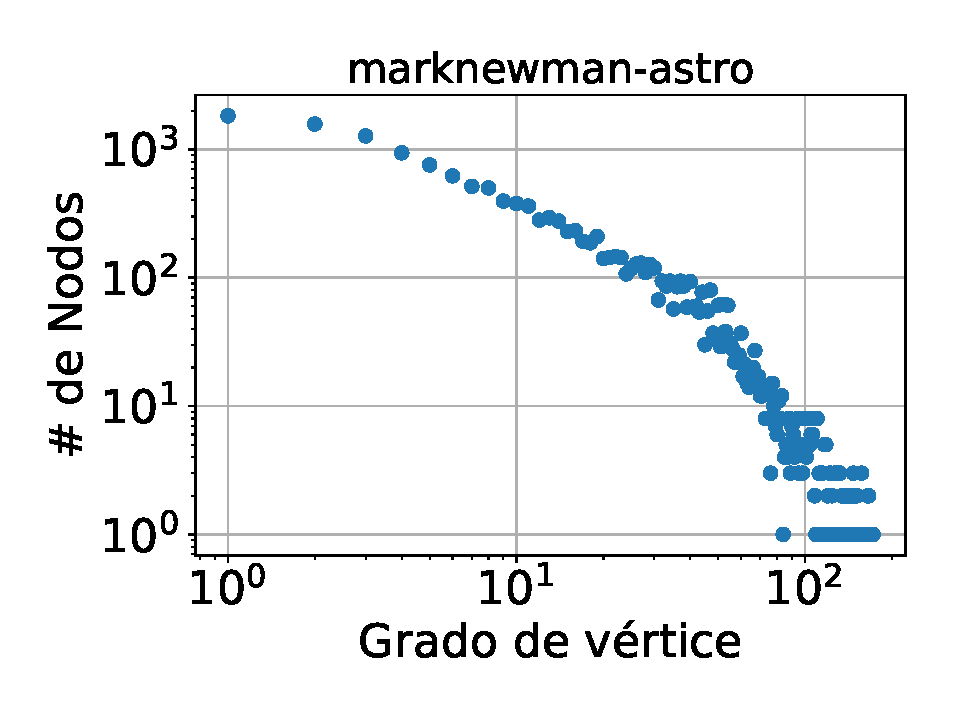
\includegraphics[width=1\linewidth]{img/grades/marknewman-astro.pdf}
    			
    			(a)
    		\end{minipage}
    		\begin{minipage}{0.45\textwidth}
    			\centering
    			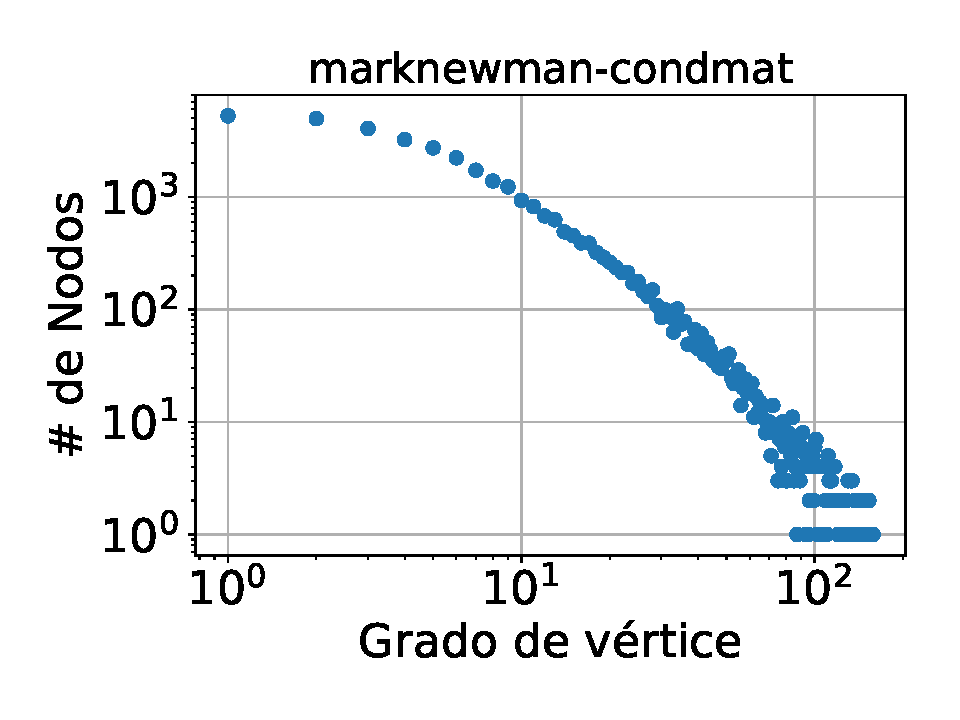
\includegraphics[width=1\linewidth]{img/grades/marknewman-condmat.pdf}
    			
    			(b)
    		\end{minipage}  		
    	\end{minipage}
    	
    	\begin{minipage}{1\textwidth}
    		\centering
    		\begin{minipage}{0.45\textwidth}
    			\centering
    			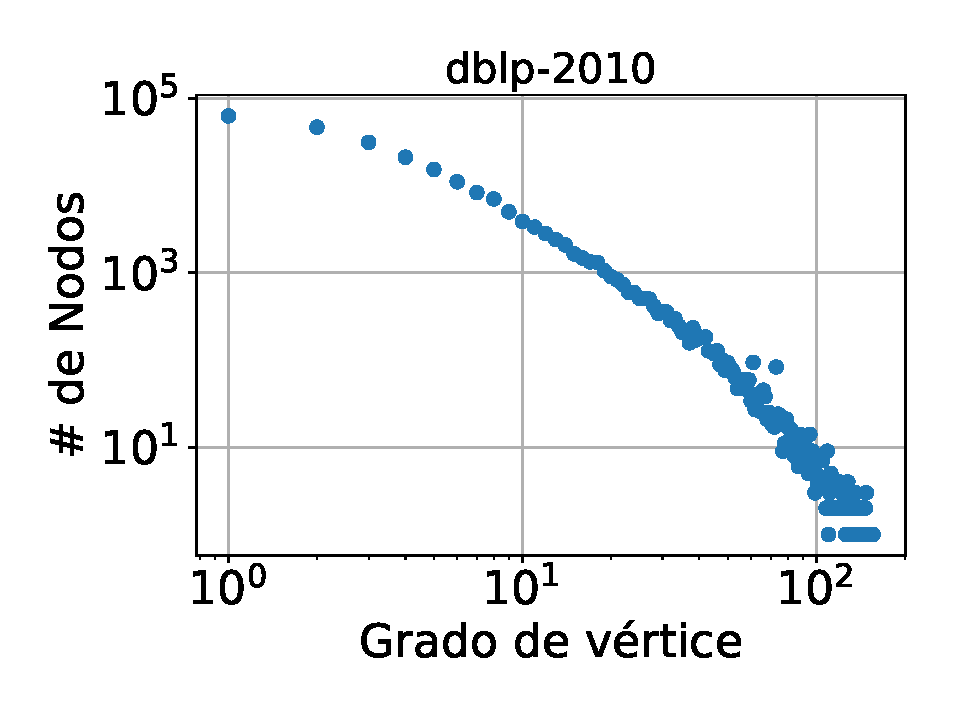
\includegraphics[width=1\linewidth]{img/grades/dblp-2010.pdf}
    			
    			(c)
    		\end{minipage}
    		\begin{minipage}{0.45\textwidth}
    			\centering
    			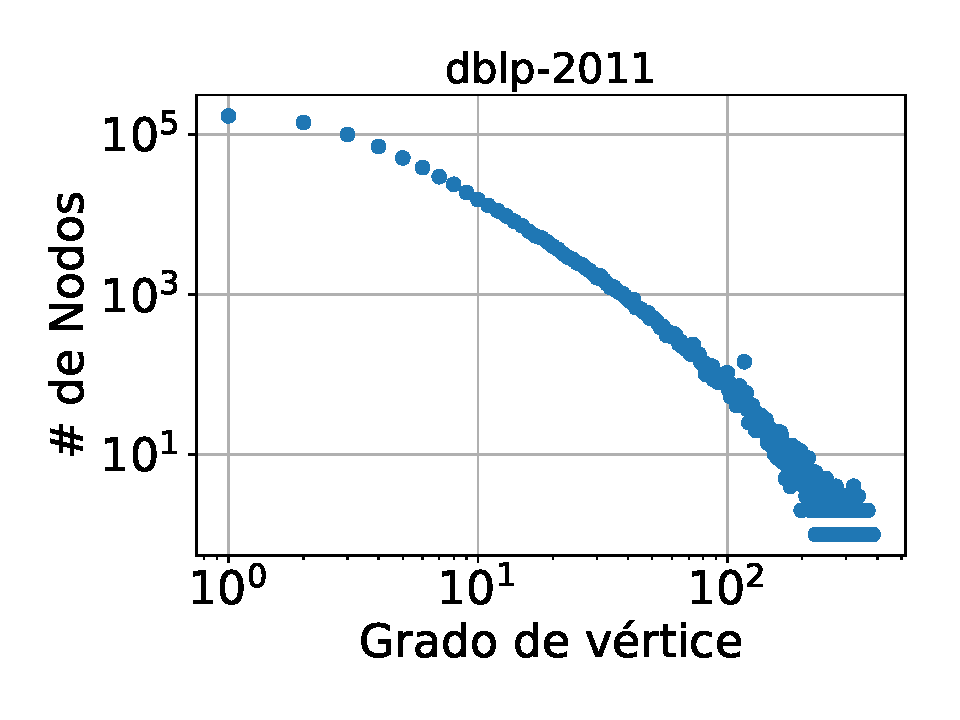
\includegraphics[width=1\linewidth]{img/grades/dblp-2011.pdf}
    			
    			(d)
    		\end{minipage}  
    	\end{minipage}
    %\caption{Distribución del grado de los vértices para cada grafo.}
    %\label{fig:grades}
%\end{figure}

%\begin{figure}%\ContinuedFloat
	%\centering
    	\begin{minipage}{1\textwidth}
    		\centering
    		\begin{minipage}{.45\textwidth}
    			\centering
    			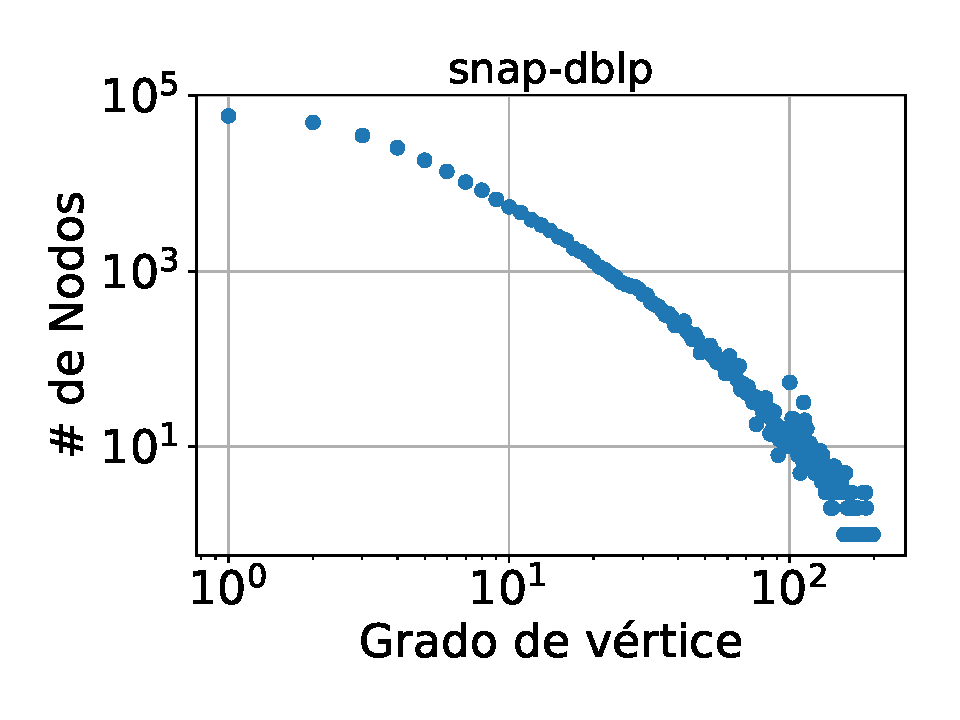
\includegraphics[width=1\linewidth]{img/grades/snap-dblp.pdf}
    			
    			(e)
    		\end{minipage}
    		\begin{minipage}{.45\textwidth}
    			\centering
    			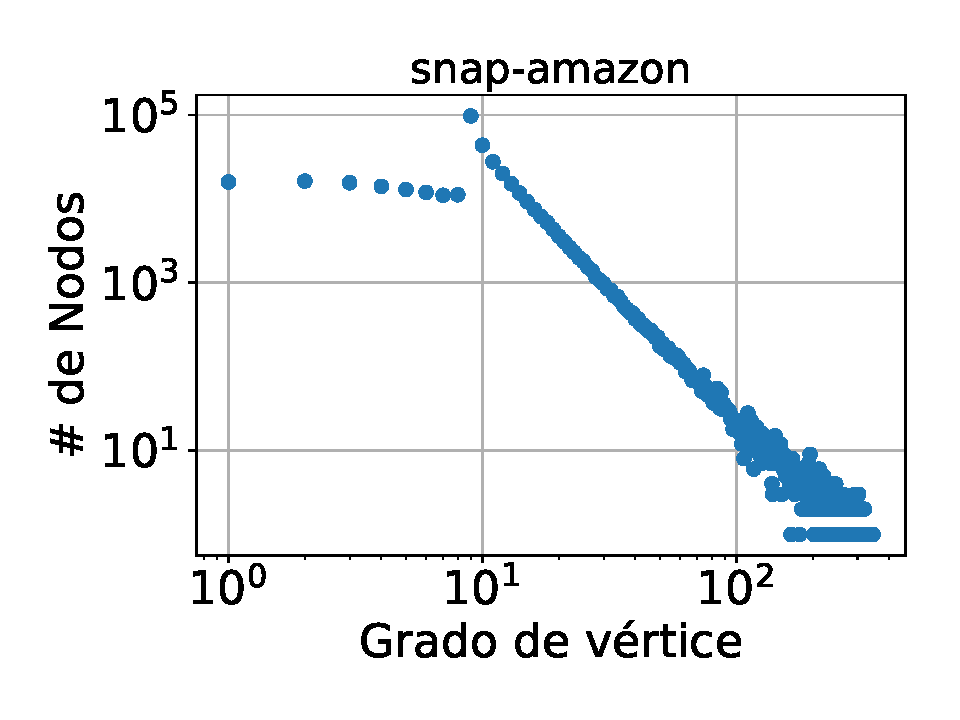
\includegraphics[width=1\linewidth]{img/grades/snap-amazon.pdf}
    			
    			(f)
    		\end{minipage}  
    	\end{minipage}
    	
    	\begin{minipage}{1\textwidth}
    		\centering
    		\begin{minipage}{0.45\textwidth}
    			\centering
    			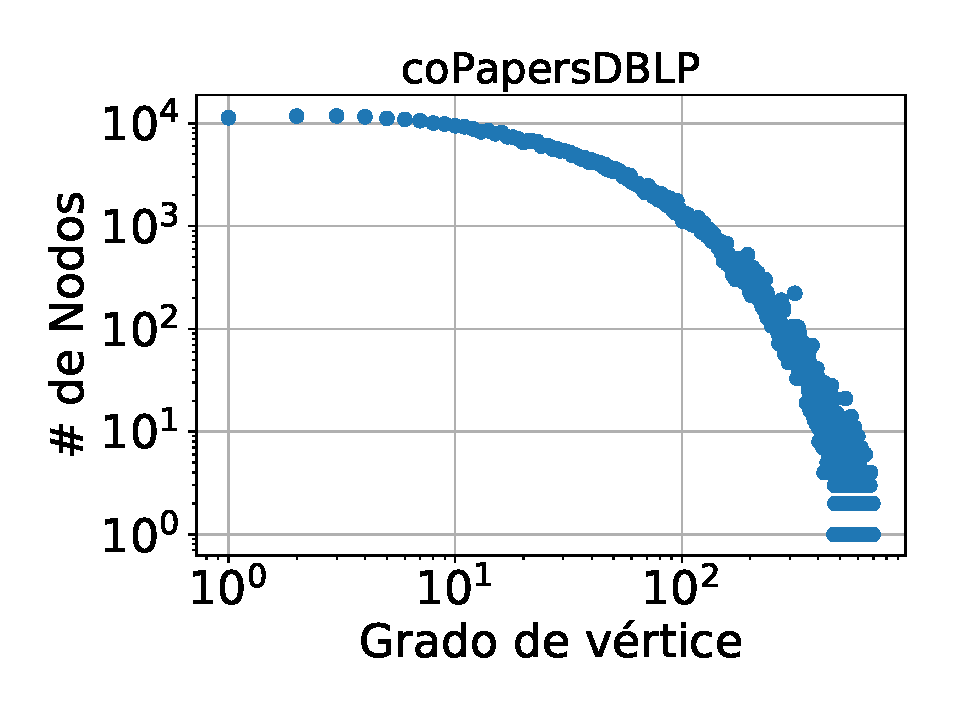
\includegraphics[width=1\linewidth]{img/grades/coPapersDBLP.pdf}
    			%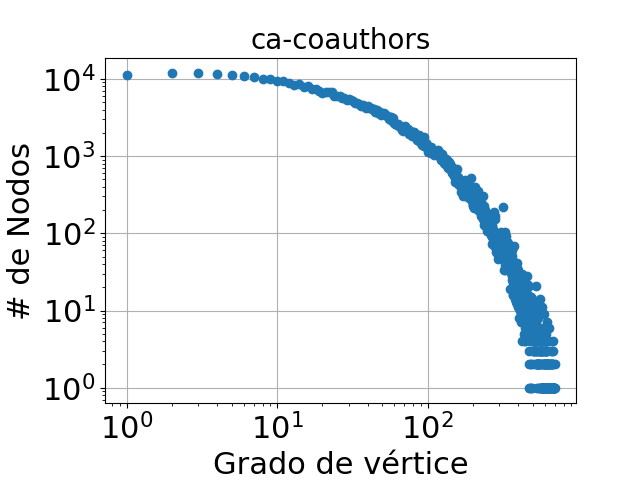
\includegraphics[width=1\linewidth]{img/grades/ca-coauthors.png}
    			
    			(g)
    		\end{minipage}
    		\begin{minipage}{0.45\textwidth}
    			\centering
    			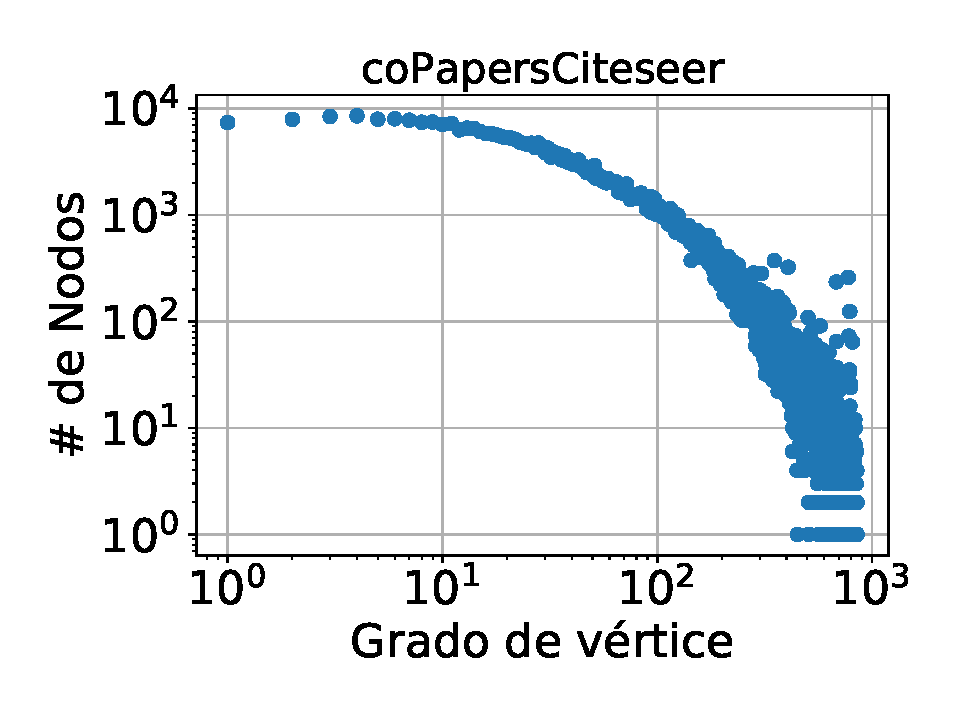
\includegraphics[width=1\linewidth]{img/grades/coPapersCiteseer.pdf}
    			
    			(h)
    		\end{minipage}  
    	\end{minipage}
    	
%    	\begin{minipage}{0.45\textwidth}
%    		\centering
%    		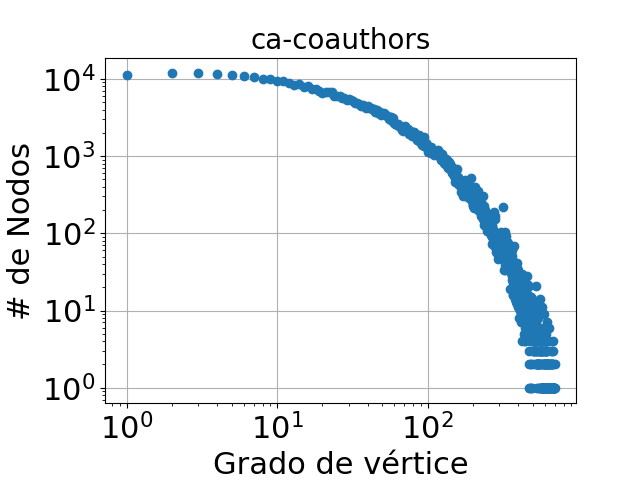
\includegraphics[width=1\linewidth]{img/grades/ca-coauthors.png}
%    		
%    		(g)
%    	\end{minipage}  
    \caption{Distribución del grado de los vértices para cada grafo.}
    \label{fig:grades}
\end{figure}

\begin{figure}
	{\normalsize
   		\centering
    	\begin{minipage}{1\textwidth}
    		\centering
    		\begin{minipage}{0.45\textwidth}
    			\centering
    			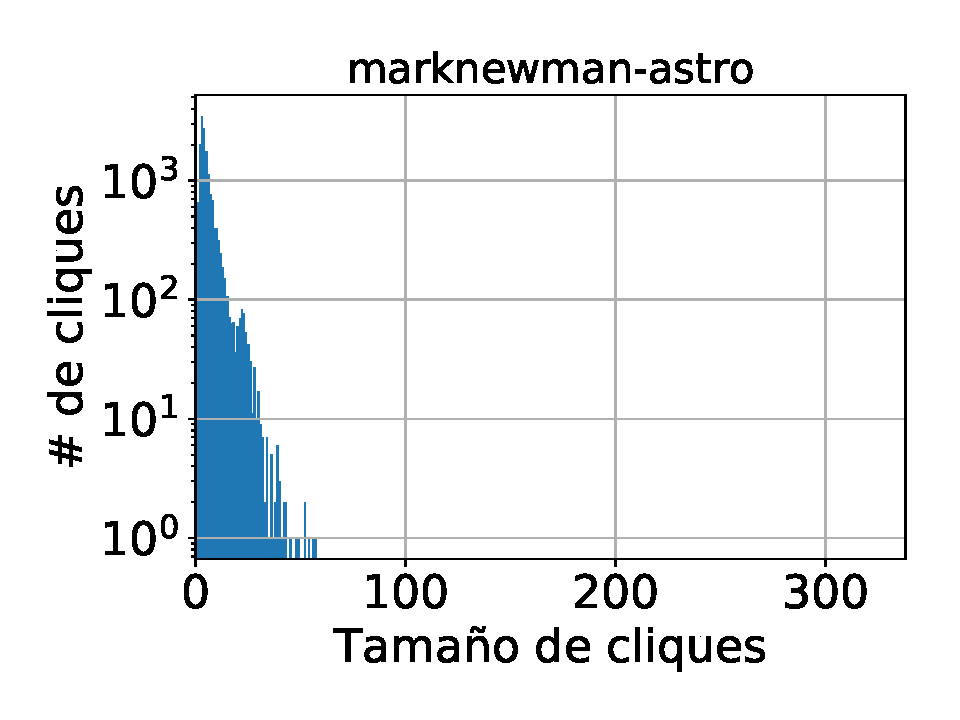
\includegraphics[width=1\linewidth]{img/cliqueDist2/marknewman-astro.pdf}
    			
    			(a)
    		\end{minipage}
    		\begin{minipage}{0.45\textwidth}
    			\centering
    			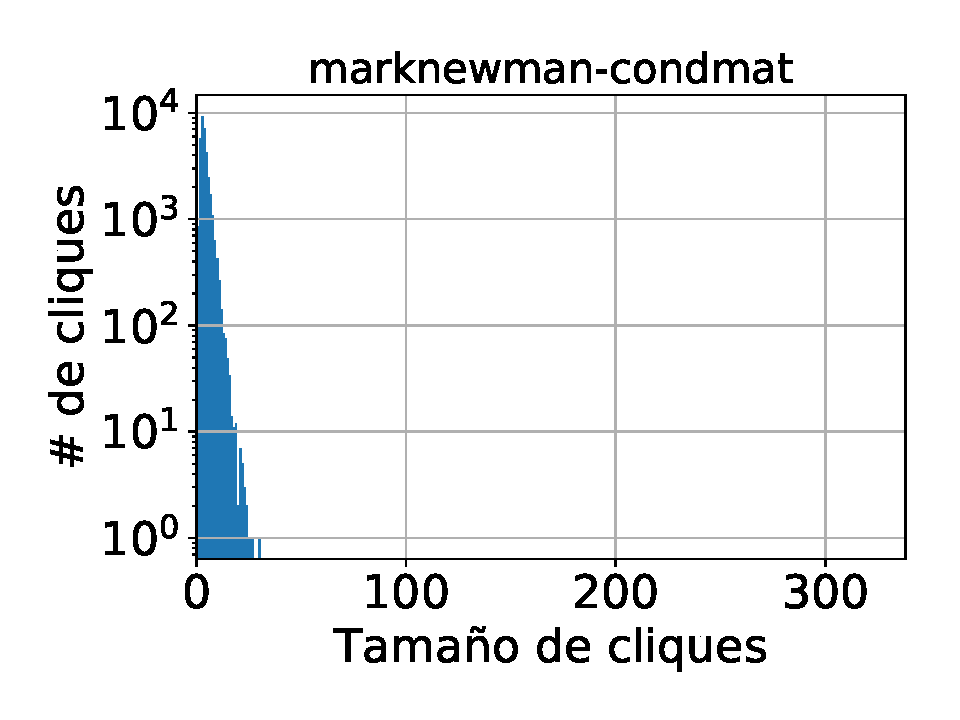
\includegraphics[width=1\linewidth]{img/cliqueDist2/marknewman-condmat.pdf}
    			
    			(b)
    		\end{minipage}  		
    	\end{minipage}
    	
    	\begin{minipage}{1\textwidth}
    		\centering
    		\begin{minipage}{0.45\textwidth}
    			\centering
    			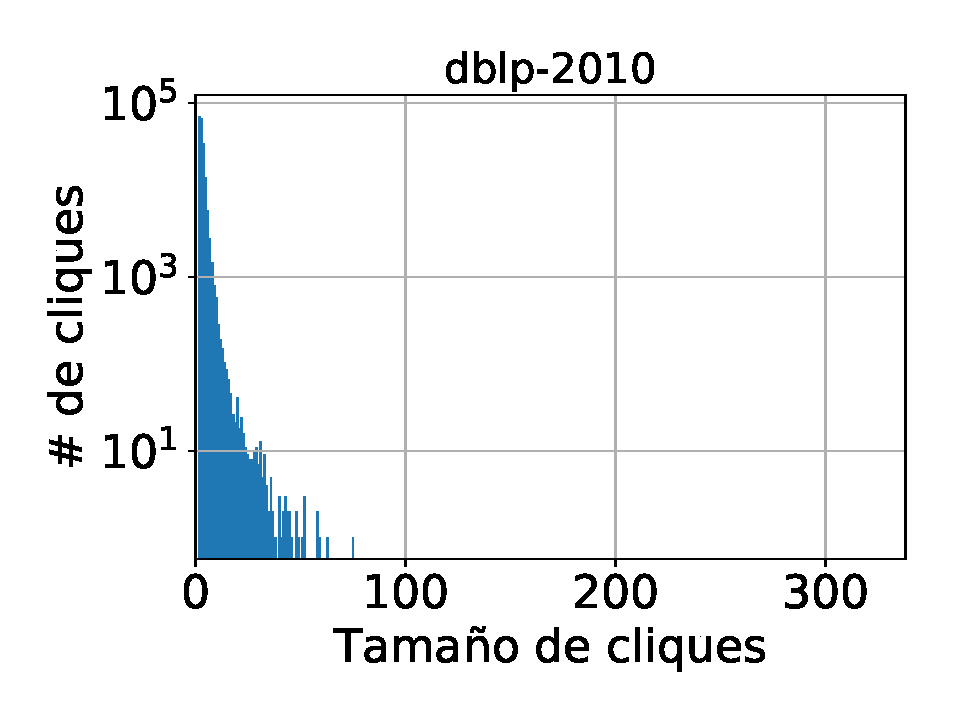
\includegraphics[width=1\linewidth]{img/cliqueDist2/dblp-2010.pdf}
    			
    			(c)
    		\end{minipage}
    		\begin{minipage}{0.45\textwidth}
    			\centering
    			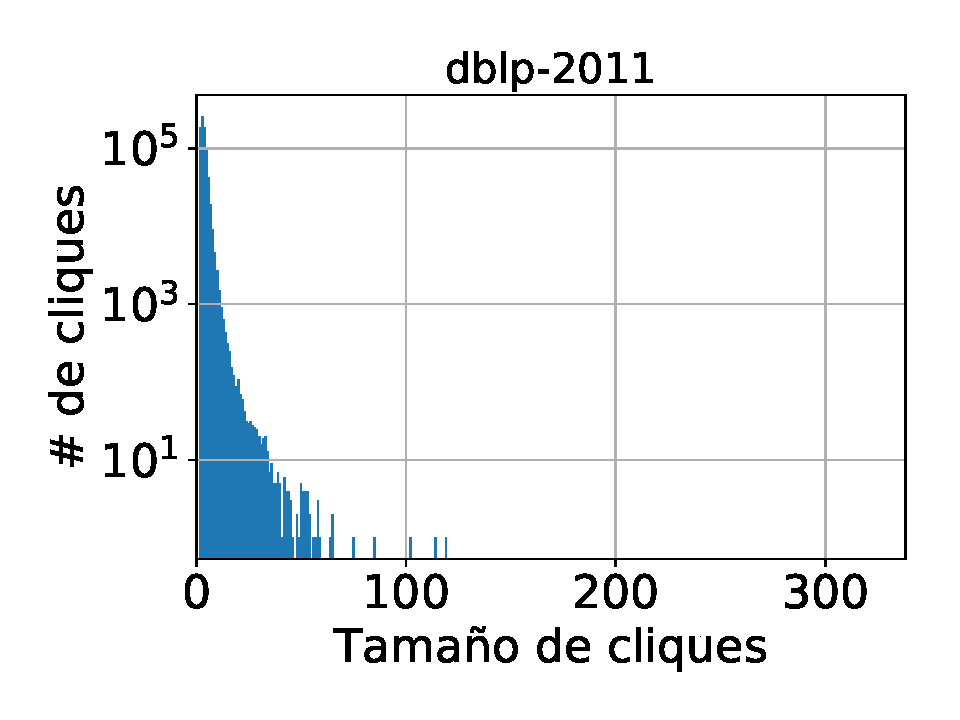
\includegraphics[width=1\linewidth]{img/cliqueDist2/dblp-2011.pdf}
    			
    			(d)
    		\end{minipage}  
    	\end{minipage}
    	
    	\begin{minipage}{1\textwidth}
    		\centering
    		\begin{minipage}{0.45\textwidth}
    			\centering
    			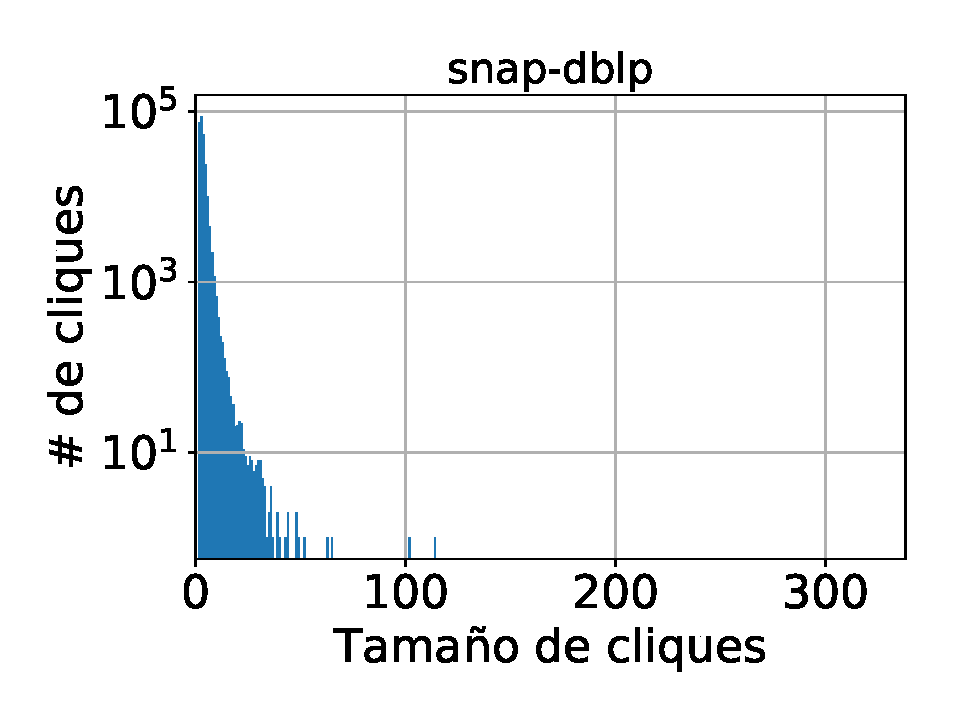
\includegraphics[width=1\linewidth]{img/cliqueDist2/snap-dblp.pdf}
    			
    			(e)
    		\end{minipage}
    		\begin{minipage}{0.45\textwidth}
    			\centering
    			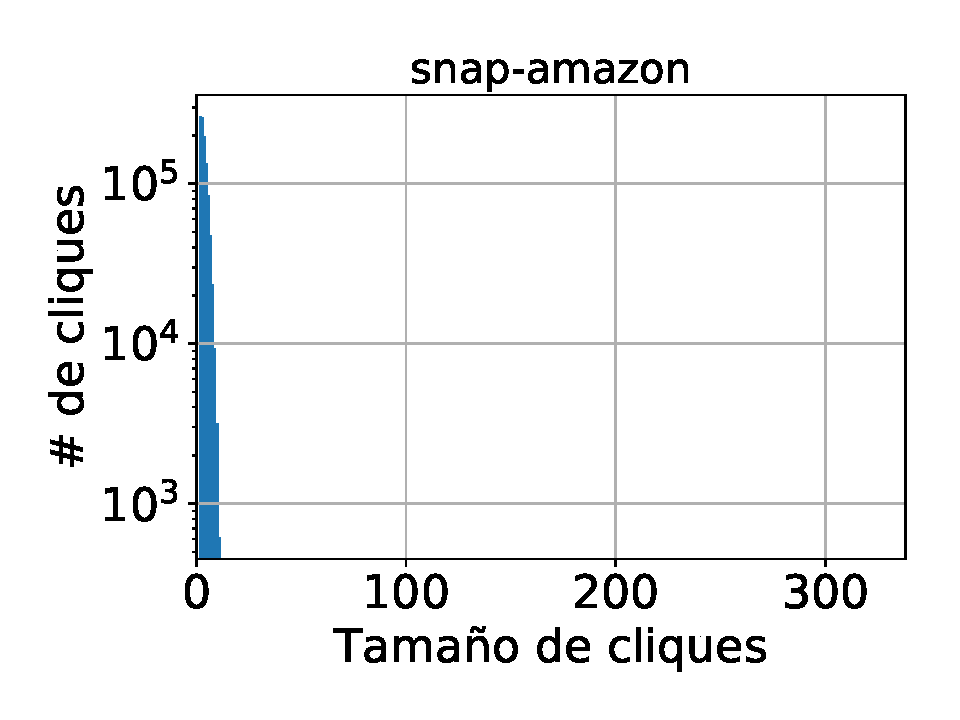
\includegraphics[width=1\linewidth]{img/cliqueDist2/snap-amazon.pdf}
    			
    			(f)
    		\end{minipage}  
    	\end{minipage}
    	
    	\begin{minipage}{1\textwidth}
    		\centering
    		\begin{minipage}{0.45\textwidth}
    			\centering
    			%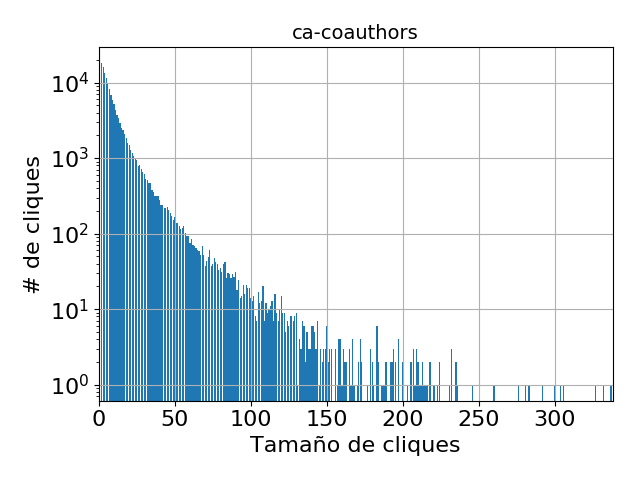
\includegraphics[width=1\linewidth]{img/cliqueDist2/ca-coauthors.png}
    			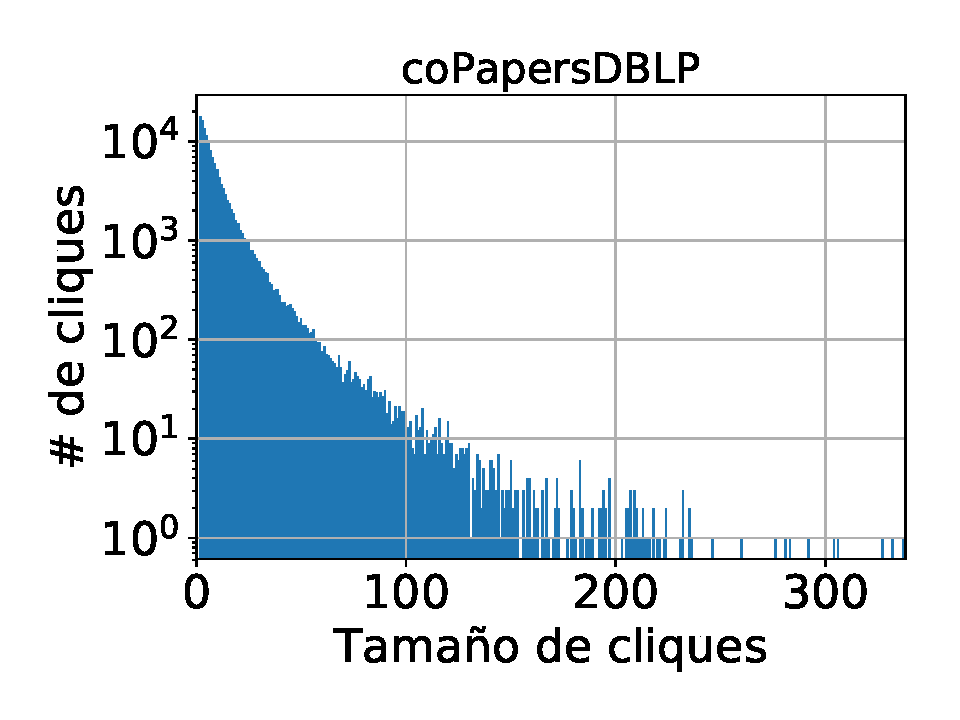
\includegraphics[width=1\linewidth]{img/cliqueDist2/coPapersDBLP.pdf}
    			
    			(g)
    		\end{minipage}
    		\begin{minipage}{0.45\textwidth}
    			\centering
    			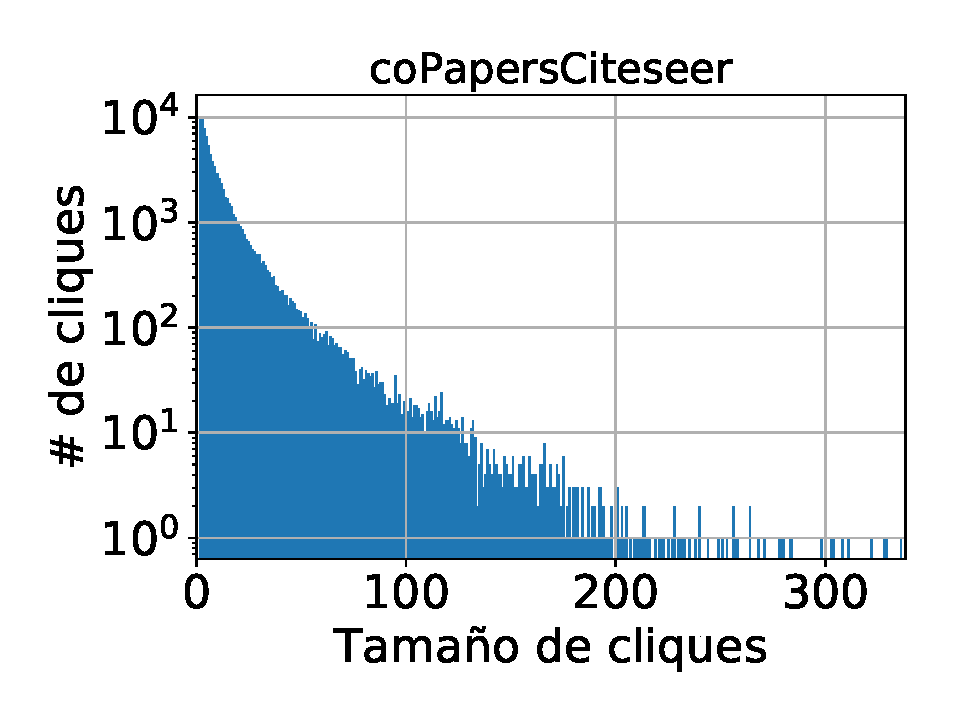
\includegraphics[width=1\linewidth]{img/cliqueDist2/coPapersCiteseer.pdf}
    			
    			(h)
    		\end{minipage}  
    	\end{minipage}
    	
%    	\begin{minipage}{0.45\textwidth}
%    		\centering
%    		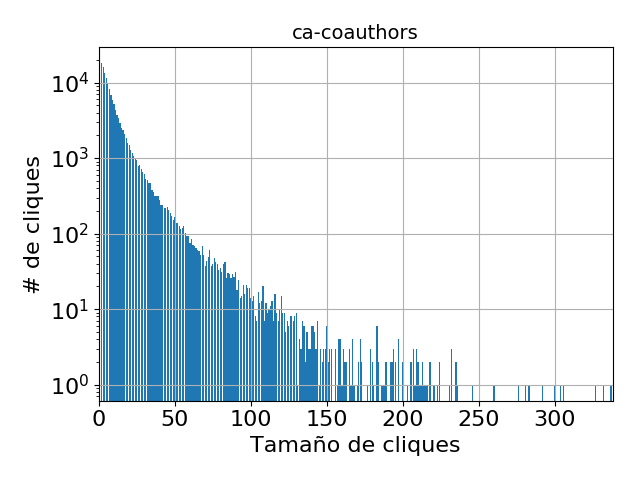
\includegraphics[width=1\linewidth]{img/cliqueDist2/ca-coauthors.png}
%    		
%    		(g)
%    	\end{minipage}
	}
     
    \caption{Distribución del tamaño de los cliques maximales para cada grafo.}
    \label{fig:cliqueDist2}
\end{figure}


La distribución de los tamaños de los cliques maximales para cada grafo se muestra en la Figura~\ref{fig:cliqueDist2}. Es importante notar que el gráfico del grafo \texttt{coPapersCiteseer} está truncado para efectos de comparación, pero tiene muy pocos cliques por sobre el límite fijado gráficamente.

La mayoría de los grafos contienen muchos cliques con menos de 50 vértices, a excepción de los grafos \texttt{snap-amazon}, \texttt{coPapersDBLP} y \texttt{coPapersCiteseer}. El primero contiene solo cliques pequeños, de no más de 20 vértices. Los otros dos grafos contienen una cantidad considerable de cliques de hasta 100 vértices. Esto permitirá contrastar los resultados del método propuesto entre grafos con distintas cantidades de cliques maximales grandes.

%\begin{figure}[p]
    	\centering
    	\begin{minipage}{1\textwidth}
    		\centering
    		\begin{minipage}{0.45\textwidth}
    			\centering
    			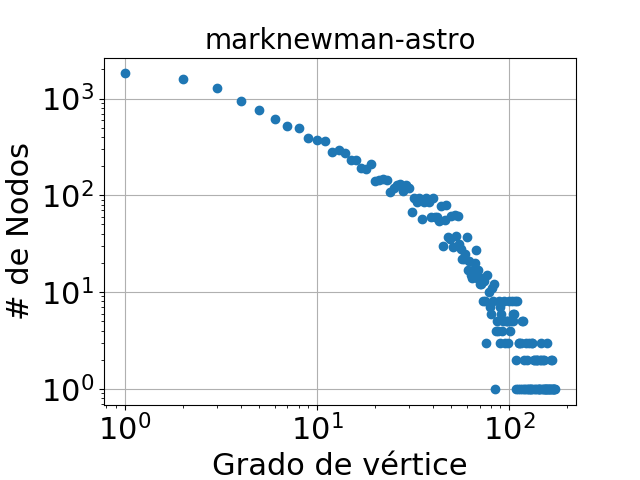
\includegraphics[width=1\linewidth]{img/grades/marknewman-astro.png}
    			
    			(a)
    		\end{minipage}
    		\begin{minipage}{0.45\textwidth}
    			\centering
    			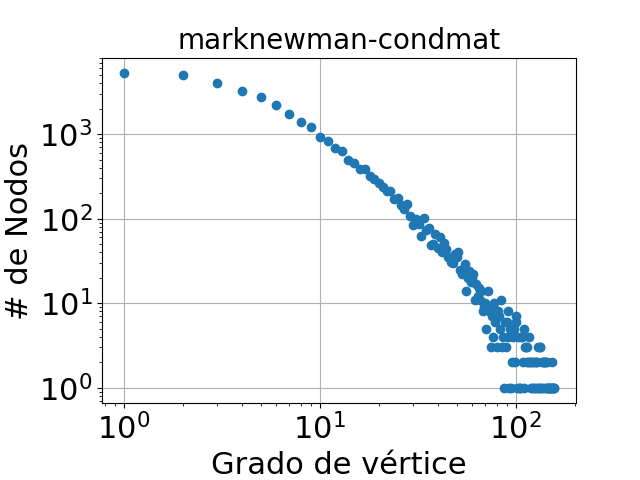
\includegraphics[width=1\linewidth]{img/grades/marknewman-condmat.png}
    			
    			(b)
    		\end{minipage}  		
    	\end{minipage}
    	
    	\begin{minipage}{1\textwidth}
    		\centering
    		\begin{minipage}{0.45\textwidth}
    			\centering
    			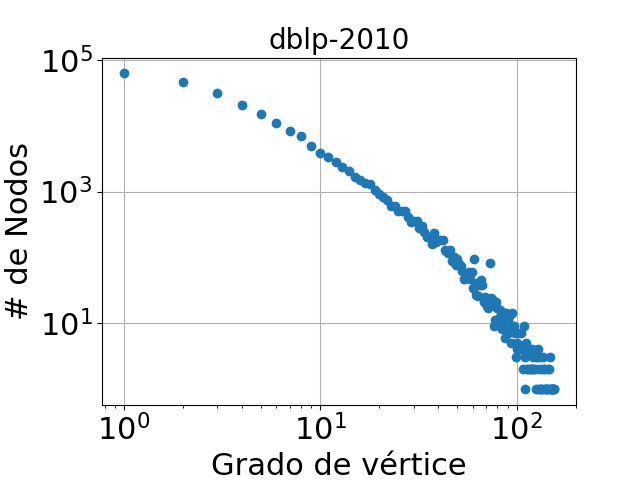
\includegraphics[width=1\linewidth]{img/grades/dblp-2010.png}
    			
    			(c)
    		\end{minipage}
    		\begin{minipage}{0.45\textwidth}
    			\centering
    			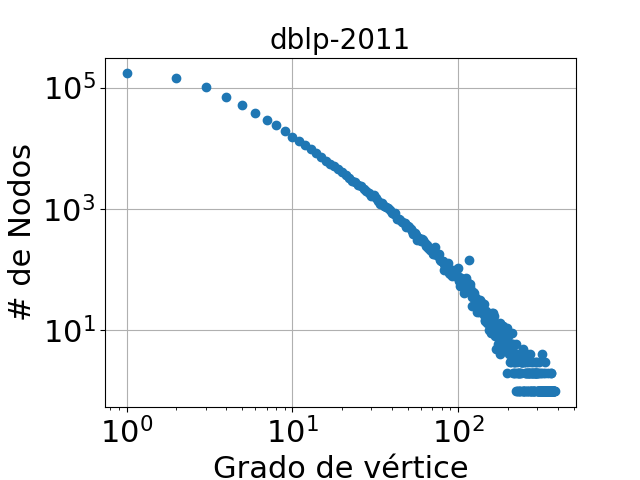
\includegraphics[width=1\linewidth]{img/grades/dblp-2011.png}
    			
    			(d)
    		\end{minipage}  
    	\end{minipage}
    	
    	\begin{minipage}{1\textwidth}
    		\centering
    		\begin{minipage}{0.45\textwidth}
    			\centering
    			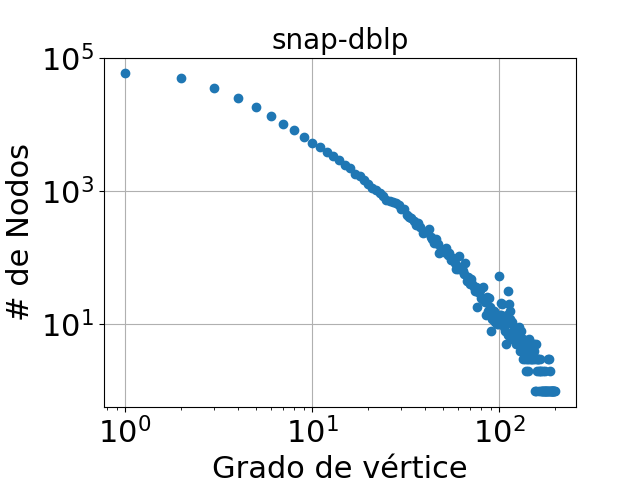
\includegraphics[width=1\linewidth]{img/grades/snap-dblp.png}
    			
    			(e)
    		\end{minipage}
    		\begin{minipage}{0.45\textwidth}
    			\centering
    			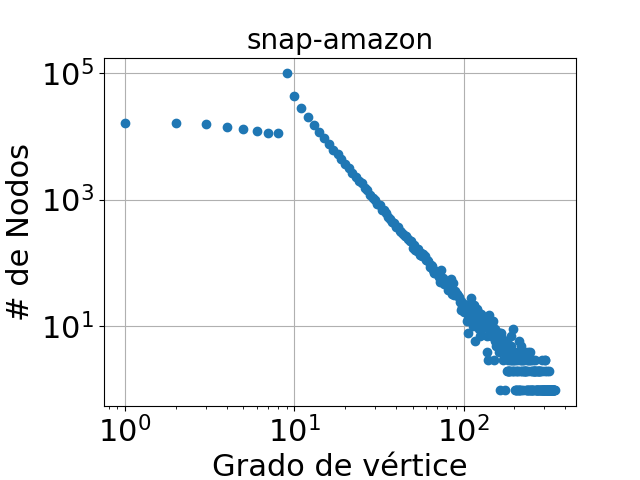
\includegraphics[width=1\linewidth]{img/grades/snap-amazon.png}
    			
    			(f)
    		\end{minipage}  
    	\end{minipage}
    	
%    	\begin{minipage}{1\textwidth}
%    		\centering
%    		\begin{minipage}{0.45\textwidth}
%    			\centering
%    			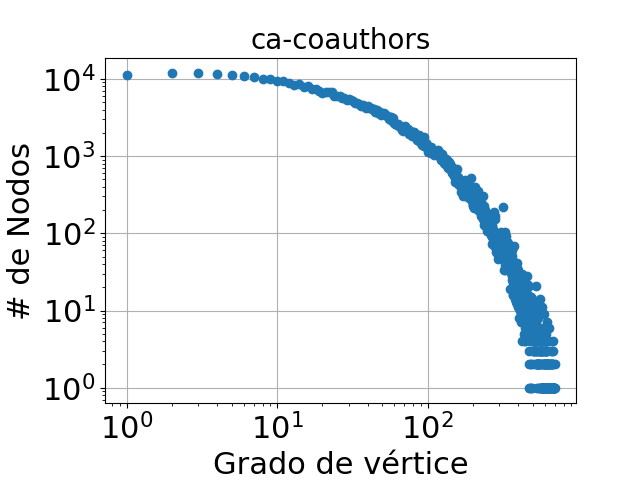
\includegraphics[width=1\linewidth]{img/grades/ca-coauthors.png}
%    			
%    			(g)
%    		\end{minipage}
%    		\begin{minipage}{0.45\textwidth}
%    			\centering
%    			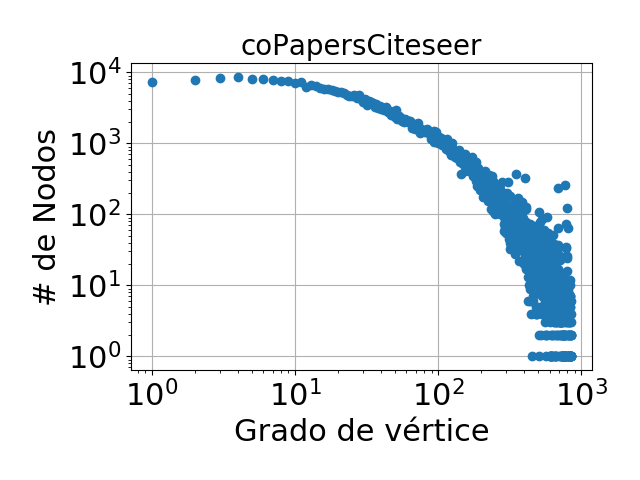
\includegraphics[width=1\linewidth]{img/grades/coPapersCiteseer.png}
%    			
%    			(h)
%    		\end{minipage}  
%    	\end{minipage}
    	
    	\begin{minipage}{0.45\textwidth}
    		\centering
    		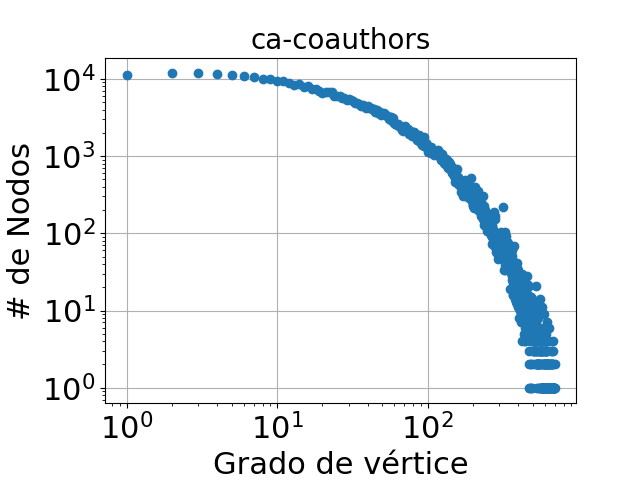
\includegraphics[width=1\linewidth]{img/grades/ca-coauthors.png}
    		
    		(g)
    	\end{minipage}  
    \caption{Distribución del grado de los vértices para cada grafo.}
    \label{fig:grades}
\end{figure}



\section{Estructura compacta}

Para generar la estructura compacta se usa \texttt{SDSL}\footnote{\url{https://github.com/simongog/sdsl-lite}} desarrollada por Gog et al.\cite{gbmp2014sea}. Las estructuras de datos sucintas a evaluar dependen del tipo de secuencia a compactar.

\begin{itemize}
	\item Para las secuencias de símbolos, se consideran las estructuras basadas en wavelet matrix (\textit{wm}) \cite{claude2015wavelet} y wavelet tree (\textit{wt}) \cite{grossi2003high}.
	\item Para la secuencia de bits, se consideran las estructuras basadas en bitmaps comprimidos de Raman, Raman y Rao (\textit{rrr}) \cite{raman2002succinct}, y Okanohara y Sadakane (\textit{sdb}) \cite{DBLP:journals/corr/abs-cs-0610001}.
	%\item Para la secuencia de bytes, se consideran las estructuras basadas en Hu-Tucker (\textit{hutu}) \cite{brisaboa2011compressed}, y Huffman (\textit{huff}) \cite{makinen2005succinct}.
\end{itemize}

La secuencia de bytes $BB$ se comprime usando código Huffman\cite{huffman1952method} directamente (ver Sección~\ref{sec:huffman}). Esto significa que la secuencia final de $BB$ se transforma en una secuencia de bits, lo que requiere actualizar los índices de inicio de sus particiones en la secuencia $Y$, y así poder decodificar directamente los bytes de las particiones correspondientes. Esto también conlleva que, por cada consulta a una partición, primero hay que decodificar todos los bytes correspondientes de esa partición antes de poder usarlos para detectar si los nodos asociados son vecinos o no.

\textcolor{red}{Creo suficiente no entrar más en detalle sobre este cambio, debido a que no es muy complejo.}

Se toman como factores de selección el nivel de compresión en bits y tanto el tiempo de reconstrucción secuencial, usando el Algoritmo~\ref{alg:sequential}, como el tiempo de acceso aleatorio al recuperar los vecinos de un millón de nodos, usando el Algoritmo~\ref{alg:neighbors}, para cada grafo y cada función de ranking con cada una de las estructuras antes planteadas.

%En la Tabla~\ref{table:sdslBitsRf} se presentan los bytes que ocupa cada estructura de datos sucintas para la función de ranking $r_{f}(u)$, en la Tabla~\ref{table:sdslBitsRc} lo equivalente para la función $r_{c}(u)$, y en la Tabla~\ref{table:sdslBitsRr} para la función $r_{r}(u)$. Se puede apreciar que en la mayoría de los casos, para las secuencias de símbolos \textit{wt} requiere menos bytes, para las secuencias de bits \textit{rrr} requiere un poco menos de la mitad de espacio que \textit{sdb}, y para las secuencias de bytes \textit{hutu} requiere menos espacio que \textit{huff}. Pero es necesario incorporar el análisis de tiempo de reconstrucción antes de seleccionar las mejores estructuras para cada secuencia.
%
%\begin{table}[t]
	%\caption{Espacio en bits de las estructuras de datos sucintos para la función $r_{f}(u)$.}
	\caption{Espacio en bytes de las estructuras de datos sucintos para la función $r_{f}(u)$.}
	\rowcolors{2}{white}{gray!10}
	\label{table:sdslBitsRf}
	\centering
	%\scriptsize
	\footnotesize
	\begin{tabular}{l||r|r||r|r||r|r||r|r}
		\toprule
		Grafo & $X_{wm}$ & $X_{wt}$ & $B_{rrr}$ & $B_{sdb}$ & $BB_{hutu}$ & $BB_{huff}$ & $Y_{wm}$ & $Y_{wt}$ \\
		\midrule
%		marknewman-astro & 507.512 & 504.568 & 17.240 & 26.416 & 450.888 & 453.128 & 44.856 & 42.744 \\
%		marknewman-condmat & 1.206.392 & 1.203.960 & 36.568 & 53.504 & 710.888 & 712.424 & 93.176 & 91.704 \\
%		dblp-2010 & 6.376.120 & 6.373.560 & 264.536 & 452.072 & 2.233.960 & 2.237.288 & 724.664 & 726.200 \\
%		dblp-2011 & 27.129.144 & 27.120.312 & 792.408 & 1.155.008 & 13.417.192 & 13.468.392 & 2.249.848 & 2.262.648 \\
%		snap-dblp & 9.157.240 & 9.150.200 & 264.152 & 391.248 & 3.717.672 & 3.718.760 & 724.024 & 725.560 \\
%		snap-amazon & 27.688.056 & 27.681.592 & 701.272 & 1.045.264 & 18.264.104 & 18.376.168 & 2.194.616 & 2.211.320 \\
%		coPapersDBLP & 16.764.152 & 16.753.208 & 388.504 & 518.376 & 4.709.416 & 4.757.608 & 810.104 & 813.240 \\
%		coPapersCiteseer & 11.574.136 & 11.566.904 & 273.496 & 379.896 & 2.883.816 & 2.896.616 & 520.056 & 520.184 \\
		marknewman-astro & 63.439 & 63.071 & 2.155 & 3.302 & 56.361 & 56.641 & 5.607 & 5.343 \\
        marknewman-condmat & 150.799 & 150.495 & 4.571 & 6.688 & 88.861 & 89.053 & 11.647 & 11.463 \\
        dblp-2010 & 797.015 & 796.695 & 33.067 & 56.509 & 279.245 & 279.661 & 90.583 & 90.775 \\
        dblp-2011 & 3.391.143 & 3.390.039 & 99.051 & 144.376 & 1.677.149 & 1.683.549 & 281.231 & 282.831 \\
        snap-dblp & 1.144.655 & 1.143.775 & 33.019 & 48.906 & 464.709 & 464.845 & 90.503 & 90.695 \\
        snap-amazon & 3.461.007 & 3.460.199 & 87.659 & 130.658 & 2.283.013 & 2.297.021 & 274.327 & 276.415 \\
        coPapersDBLP & 2.095.519 & 2.094.151 & 48.563 & 64.797 & 588.677 & 594.701 & 101.263 & 101.655 \\
        coPapersCiteseer & 1.446.767 & 1.445.863 & 34.187 & 47.487 & 360.477 & 362.077 & 65.007 & 65.023 \\
        \bottomrule
	\end{tabular}
\end{table}

%\begin{table}[t]
	%\caption{Espacio en bits de las estructuras de datos sucintos para la función $r_{c}(u)$.}
	\caption{Espacio en bytes de las estructuras de datos sucintos para la función $r_{c}(u)$.}
	\rowcolors{2}{white}{gray!10}
	\label{table:sdslBitsRc}
	\centering
	%\scriptsize
	\footnotesize
	\begin{tabular}{l||r|r||r|r||r|r||r|r}
		\toprule
		Grafo & $X_{wm}$ & $X_{wt}$ & $B_{rrr}$ & $B_{sdb}$ & $BB_{hutu}$ & $BB_{huff}$ & $Y_{wm}$ & $Y_{wt}$ \\
		\midrule
%		marknewman-astro & 520.504 & 517.880 & 17.368 & 29.056 & 443.720 & 446.280 & 48.184 & 45.880 \\
%        marknewman-condmat & 1.225.016 & 1.222.584 & 36.504 & 57.048 & 704.520 & 706.760 & 96.696 & 94.904 \\
%        dblp-2010 & 6.721.336 & 6.715.640 & 264.792 & 455.976 & 2.237.544 & 2.243.368 & 762.296 & 762.552 \\
%        dblp-2011 & 28.130.424 & 28.117.304 & 800.664 & 1.172.680 & 13.362.280 & 13.419.688 & 2.347.192 & 2.359.928 \\
%        snap-dblp & 9.337.976 & 9.329.784 & 267.864 & 398.040 & 3.710.120 & 3.712.424 & 756.792 & 760.952 \\
%        snap-amazon & 28.092.216 & 28.087.160 & 720.600 & 1.074.328 & 18.155.816 & 18.265.640 & 2.298.040 & 2.316.216 \\
%        coPapersDBLP & 17.791.928 & 17.784.056 & 419.992 & 554.488 & 4.341.608 & 4.370.536 & 912.184 & 915.448 \\
%        coPapersCiteseer & 12.215.544 & 12.207.416 & 291.416 & 406.464 & 2.672.680 & 2.708.584 & 586.552 & 587.640 \\
		marknewman-astro & 65.063 & 64.735 & 2.171 & 3.632 & 55.465 & 55.785 & 6.023 & 5.735 \\
        marknewman-condmat & 153.127 & 152.823 & 4.563 & 7.131 & 88.065 & 88.345 & 12.087 & 11.863 \\
        dblp-2010 & 840.167 & 839.455 & 33.099 & 56.997 & 279.693 & 280.421 & 95.287 & 95.319 \\
        dblp-2011 & 3.516.303 & 3.514.663 & 100.083 & 146.585 & 1.670.285 & 1.677.461 & 293.399 & 294.991 \\
        snap-dblp & 1.167.247 & 1.166.223 & 33.483 & 49.755 & 463.765 & 464.053 & 94.599 & 95.119 \\
        snap-amazon & 3.511.527 & 3.510.895 & 90.075 & 134.291 & 2.269.477 & 2.283.205 & 287.255 & 289.527 \\
        coPapersDBLP & 2.223.991 & 2.223.007 & 52.499 & 69.311 & 542.701 & 546.317 & 114.023 & 114.431 \\
        coPapersCiteseer & 1.526.943 & 1.525.927 & 36.427 & 50.808 & 334.085 & 338.573 & 73.319 & 73.455 \\
        \bottomrule
	\end{tabular}
\end{table}










%\begin{table}[t]
	%\caption{Espacio en bits de las estructuras de datos sucintos para la función $r_{r}(u)$.}
	\caption{Espacio en bytes de las estructuras de datos sucintos para la función $r_{r}(u)$.}
	\rowcolors{2}{white}{gray!10}
	\label{table:sdslBitsRr}
	\centering
	%\scriptsize
	\footnotesize
	\begin{tabular}{l||r|r||r|r||r|r||r|r}
		\toprule
		Grafo & $X_{wm}$ & $X_{wt}$ & $B_{rrr}$ & $B_{sdb}$ & $BB_{hutu}$ & $BB_{huff}$ & $Y_{wm}$ & $Y_{wt}$ \\
		\midrule
%		marknewman-astro & 657.528 & 655.032 & 26.200 & 37.568 & 331.912 & 334.920 & 64.568 & 62.904 \\
%		marknewman-condmat & 1.494.392 & 1.492.024 & 61.720 & 85.536 & 466.472 & 470.504 & 158.328 & 156.152 \\
%		dblp-2010 & 7.412.280 & 7.407.480 & 430.424 & 638.616 & 1.088.424 & 1.097.128 & 1.207.864 & 1.206.520 \\
%		dblp-2011 & 32.853.944 & 32.828.536 & 1.499.800 & 1.963.152 & 7.279.144 & 7.397.224 & 4.497.976 & 4.508.216 \\
%		snap-dblp & 11.034.360 & 11.027.576 & 450.520 & 706.304 & 2.321.960 & 2.341.736 & 1.308.280 & 1.308.728 \\
%		snap-amazon & 32.730.680 & 32.719.032 & 1.052.056 & 1.402.544 & 14.134.568 & 14.330.472 & 3.394.104 & 3.410.680 \\
%		coPapersDBLP & 21.342.328 & 21.329.848 & 573.528 & 788.080 & 1.439.880 & 1.453.192 & 1.091.192 & 1.089.528 \\
%		coPapersCiteseer & 14.953.400 & 14.943.992 & 392.984 & 521.640 & 928.072 & 914.632 & 695.480 & 693.432 \\
		marknewman-astro & 82.191 & 81.879 & 3.275 & 4.696 & 41.489 & 41.865 & 8.071 & 7.863 \\
        marknewman-condmat & 186.799 & 186.503 & 7.715 & 10.692 & 58.309 & 58.813 & 19.791 & 19.519 \\
        dblp-2010 & 926.535 & 925.935 & 53.803 & 79.827 & 136.053 & 137.141 & 150.983 & 150.815 \\
        dblp-2011 & 4.106.743 & 4.103.567 & 187.475 & 245.394 & 909.893 & 924.653 & 562.247 & 563.527 \\
        snap-dblp & 1.379.295 & 1.378.447 & 56.315 & 88.288 & 290.245 & 292.717 & 163.535 & 163.591 \\
        snap-amazon & 4.091.335 & 4.089.879 & 131.507 & 175.318 & 1.766.821 & 1.791.309 & 424.263 & 426.335 \\
        coPapersDBLP & 2.667.791 & 2.666.231 & 71.691 & 98.510 & 179.985 & 181.649 & 136.399 & 136.191 \\
        coPapersCiteseer & 1.869.175 & 1.867.999 & 49.123 & 65.205 & 116.009 & 114.329 & 86.935 & 86.679 \\
        \bottomrule
	\end{tabular}
\end{table}










\textcolor{red}{Aquí antes mostraba las tablas con los tamaños en bytes de cada estructura compacta. Las eliminé, ya que creo no aportan en mucho comparado con la comparativa entre BPE y espacio.}

Para ello, se decide construir la estructura compacta para cada grafo y cada función de ranking, con todas las posibles combinaciones para las secuencias. En la Figura~\ref{fig:sdslBPE2}, Figura~\ref{fig:sdslBPE3}, Figura~\ref{fig:sdslBPE4}, y Figura~\ref{fig:sdslBPE5}, se compara para cada grafo el BPE de las ocho posibles combinaciones para cada función de ranking con respecto al tiempo secuencial de reconstrucción del grafo. Y en la Figura~\ref{fig:sdslBPEAle2}, Figura~\ref{fig:sdslBPEAle3}, Figura~\ref{fig:sdslBPEAle4} y Figura~\ref{fig:sdslBPEAle5}, el BPE con respecto al tiempo de acceso aleatorio al recuperar los vecinos de un millón de nodos.

\textcolor{red}{No estoy seguro que esta sea la mejor manera de anotar tantas figuras.}

En la mayoría de los casos, la estructura que presenta la mejor relación entre BPE y tiempos es la de secuencias de símbolos con \textit{wm}, secuencia de bytes con \textit{hutu}, y secuencia de bits con \textit{sdb}.  Las opciones que presentan menores tiempos aumentan en BPE, y viceversa. Por tanto, se elige esta combinación de estructuras de secuencias como la estructura compacta a desarrollar.

\begin{figure}
    	\centering
    	\begin{minipage}{1\textwidth}
    			\centering
    			\begin{minipage}{0.8\textwidth}
    				\centering
    				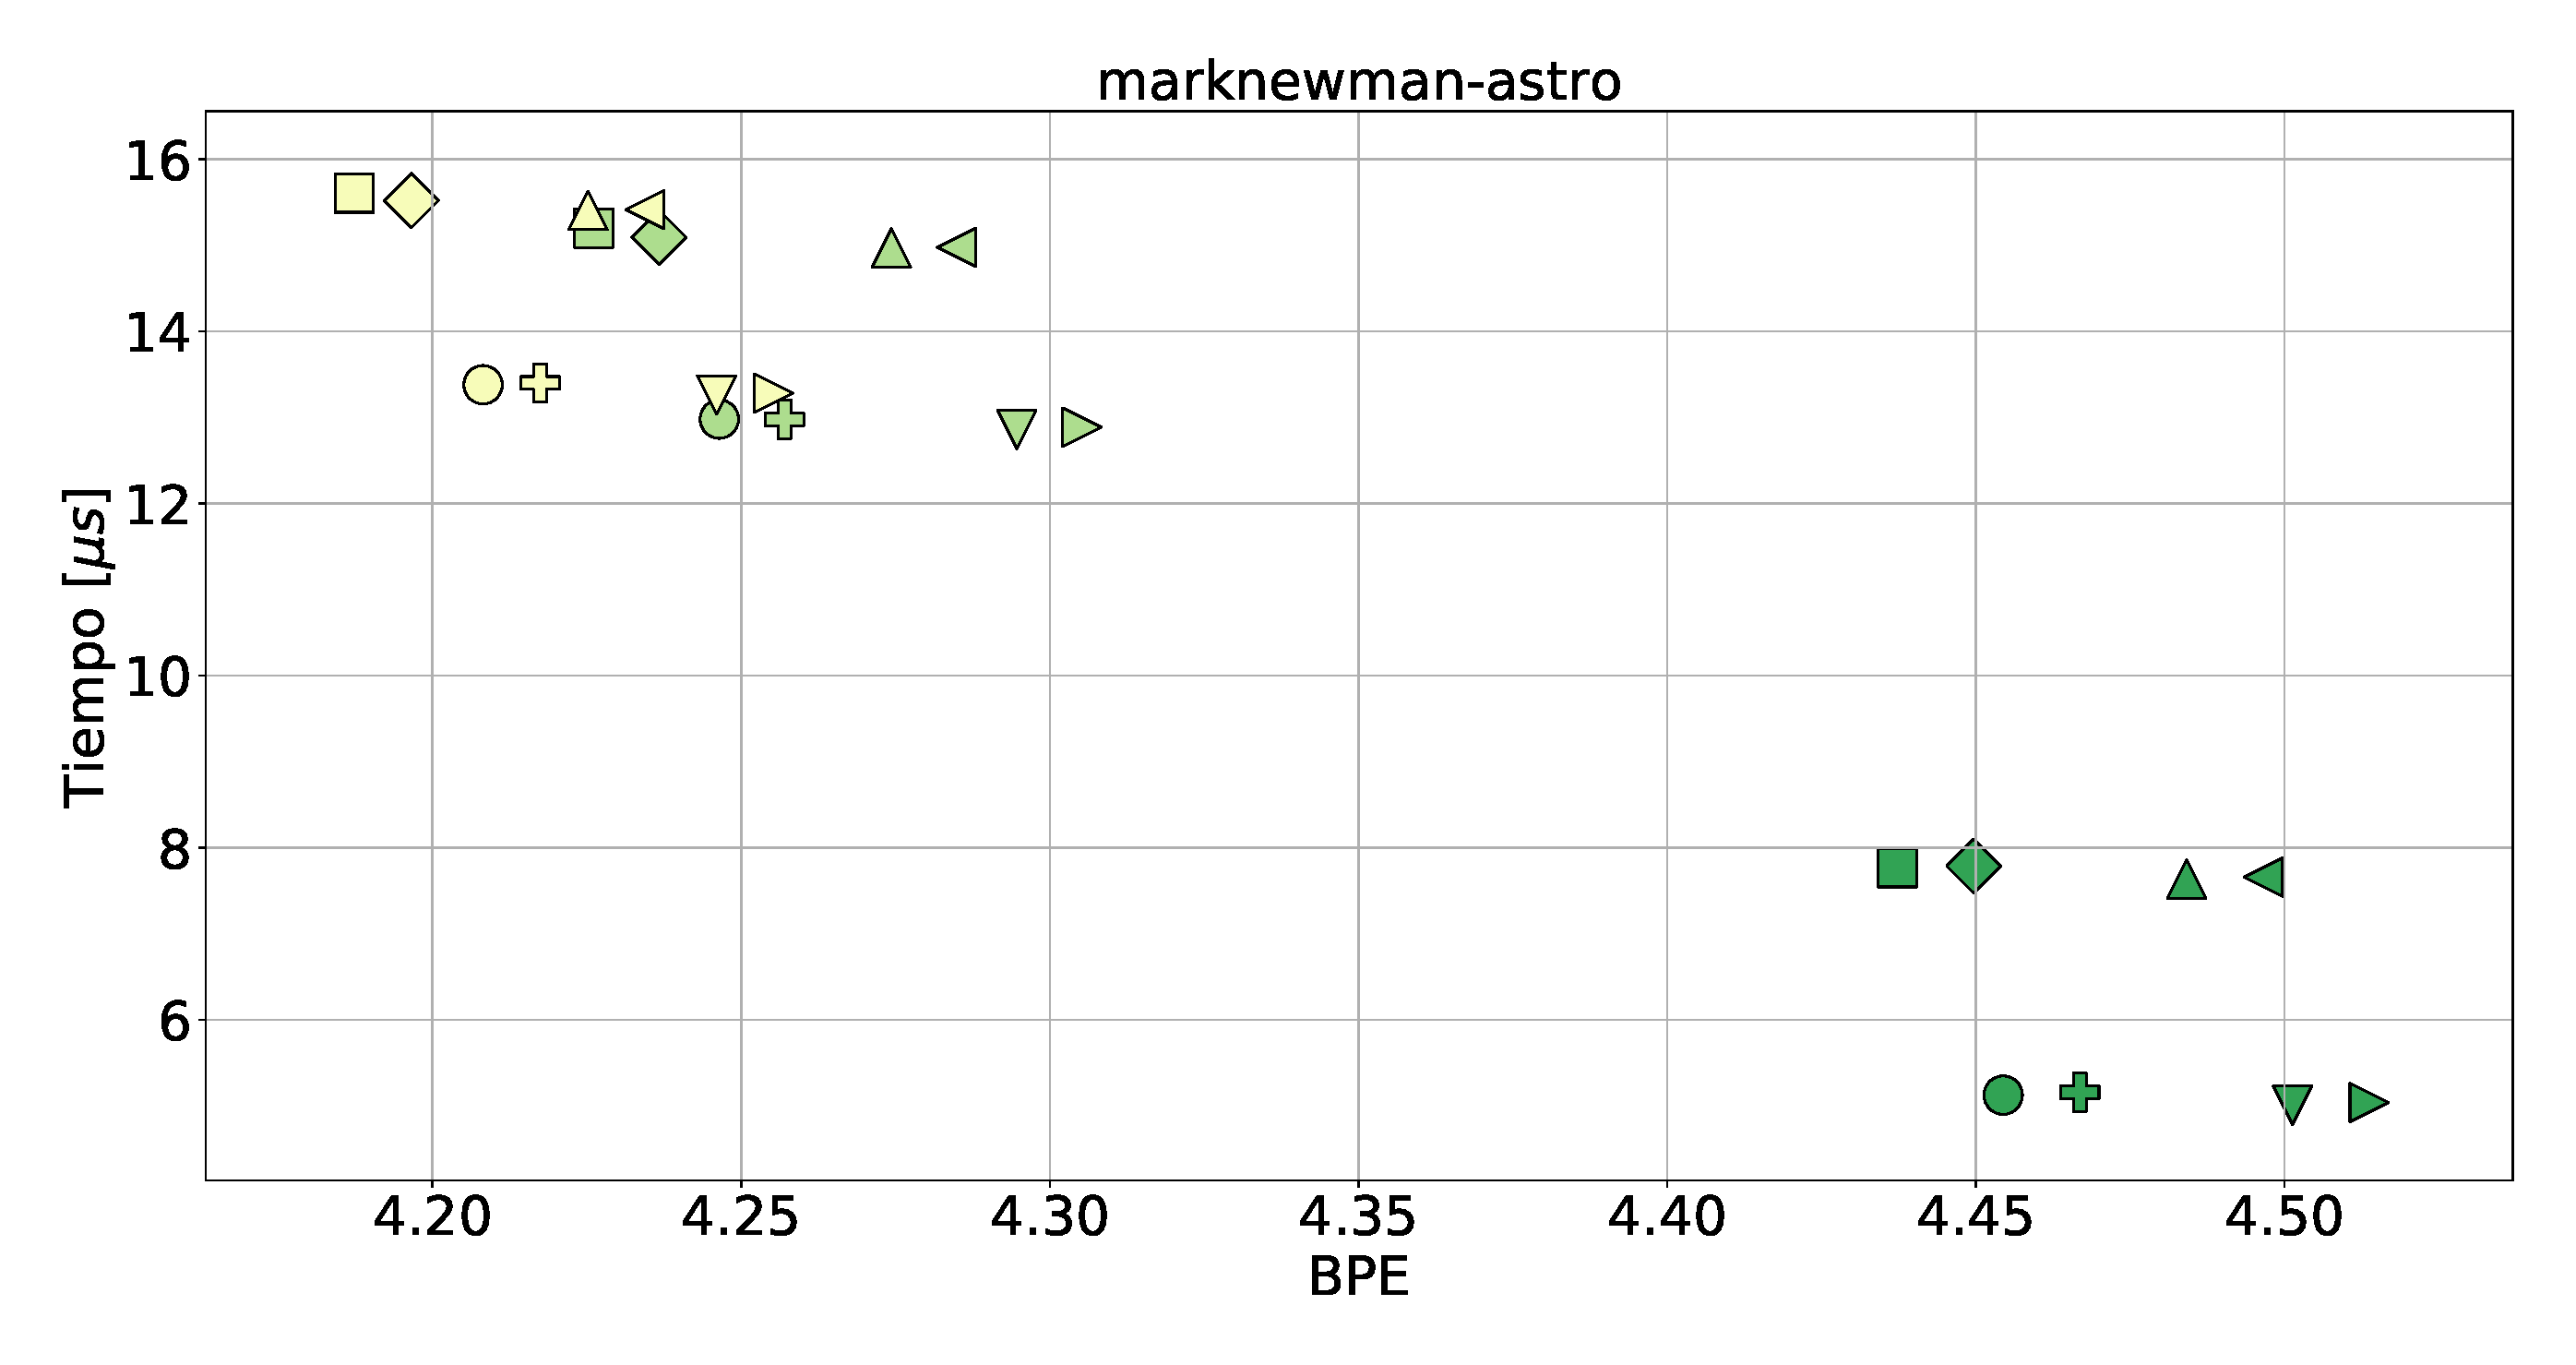
\includegraphics[width=1\linewidth]{img/sdsl/aleatorioBig/marknewman-astro.pdf}
    			\end{minipage}
    			\begin{minipage}{0.15\textwidth}
    				\centering
    				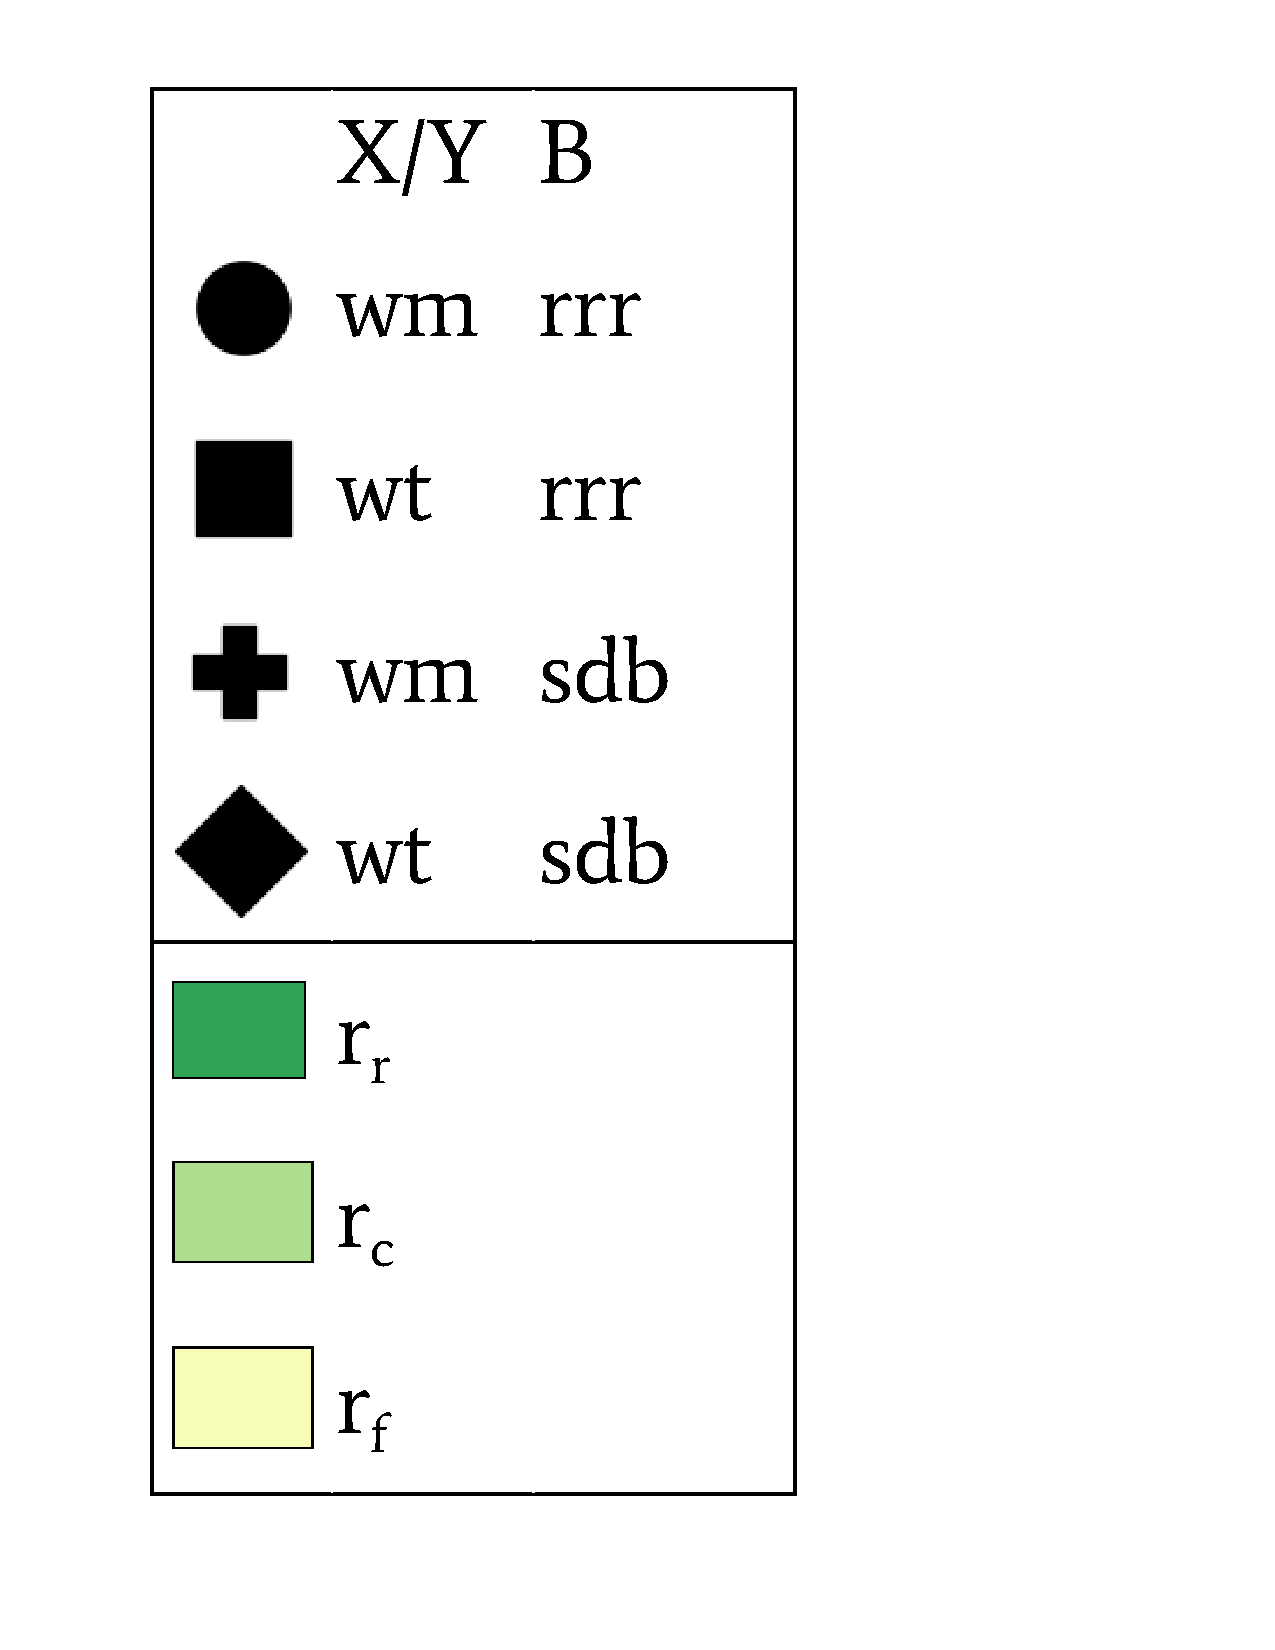
\includegraphics[scale=.22, clip, trim=70 0 0 0]{img/sdsl/label.pdf}
    			\end{minipage}
    			
    			(a)		
    	\end{minipage}
    	
       	\begin{minipage}{1\textwidth}
    			\centering
    			\begin{minipage}{0.8\textwidth}
    				\centering
    				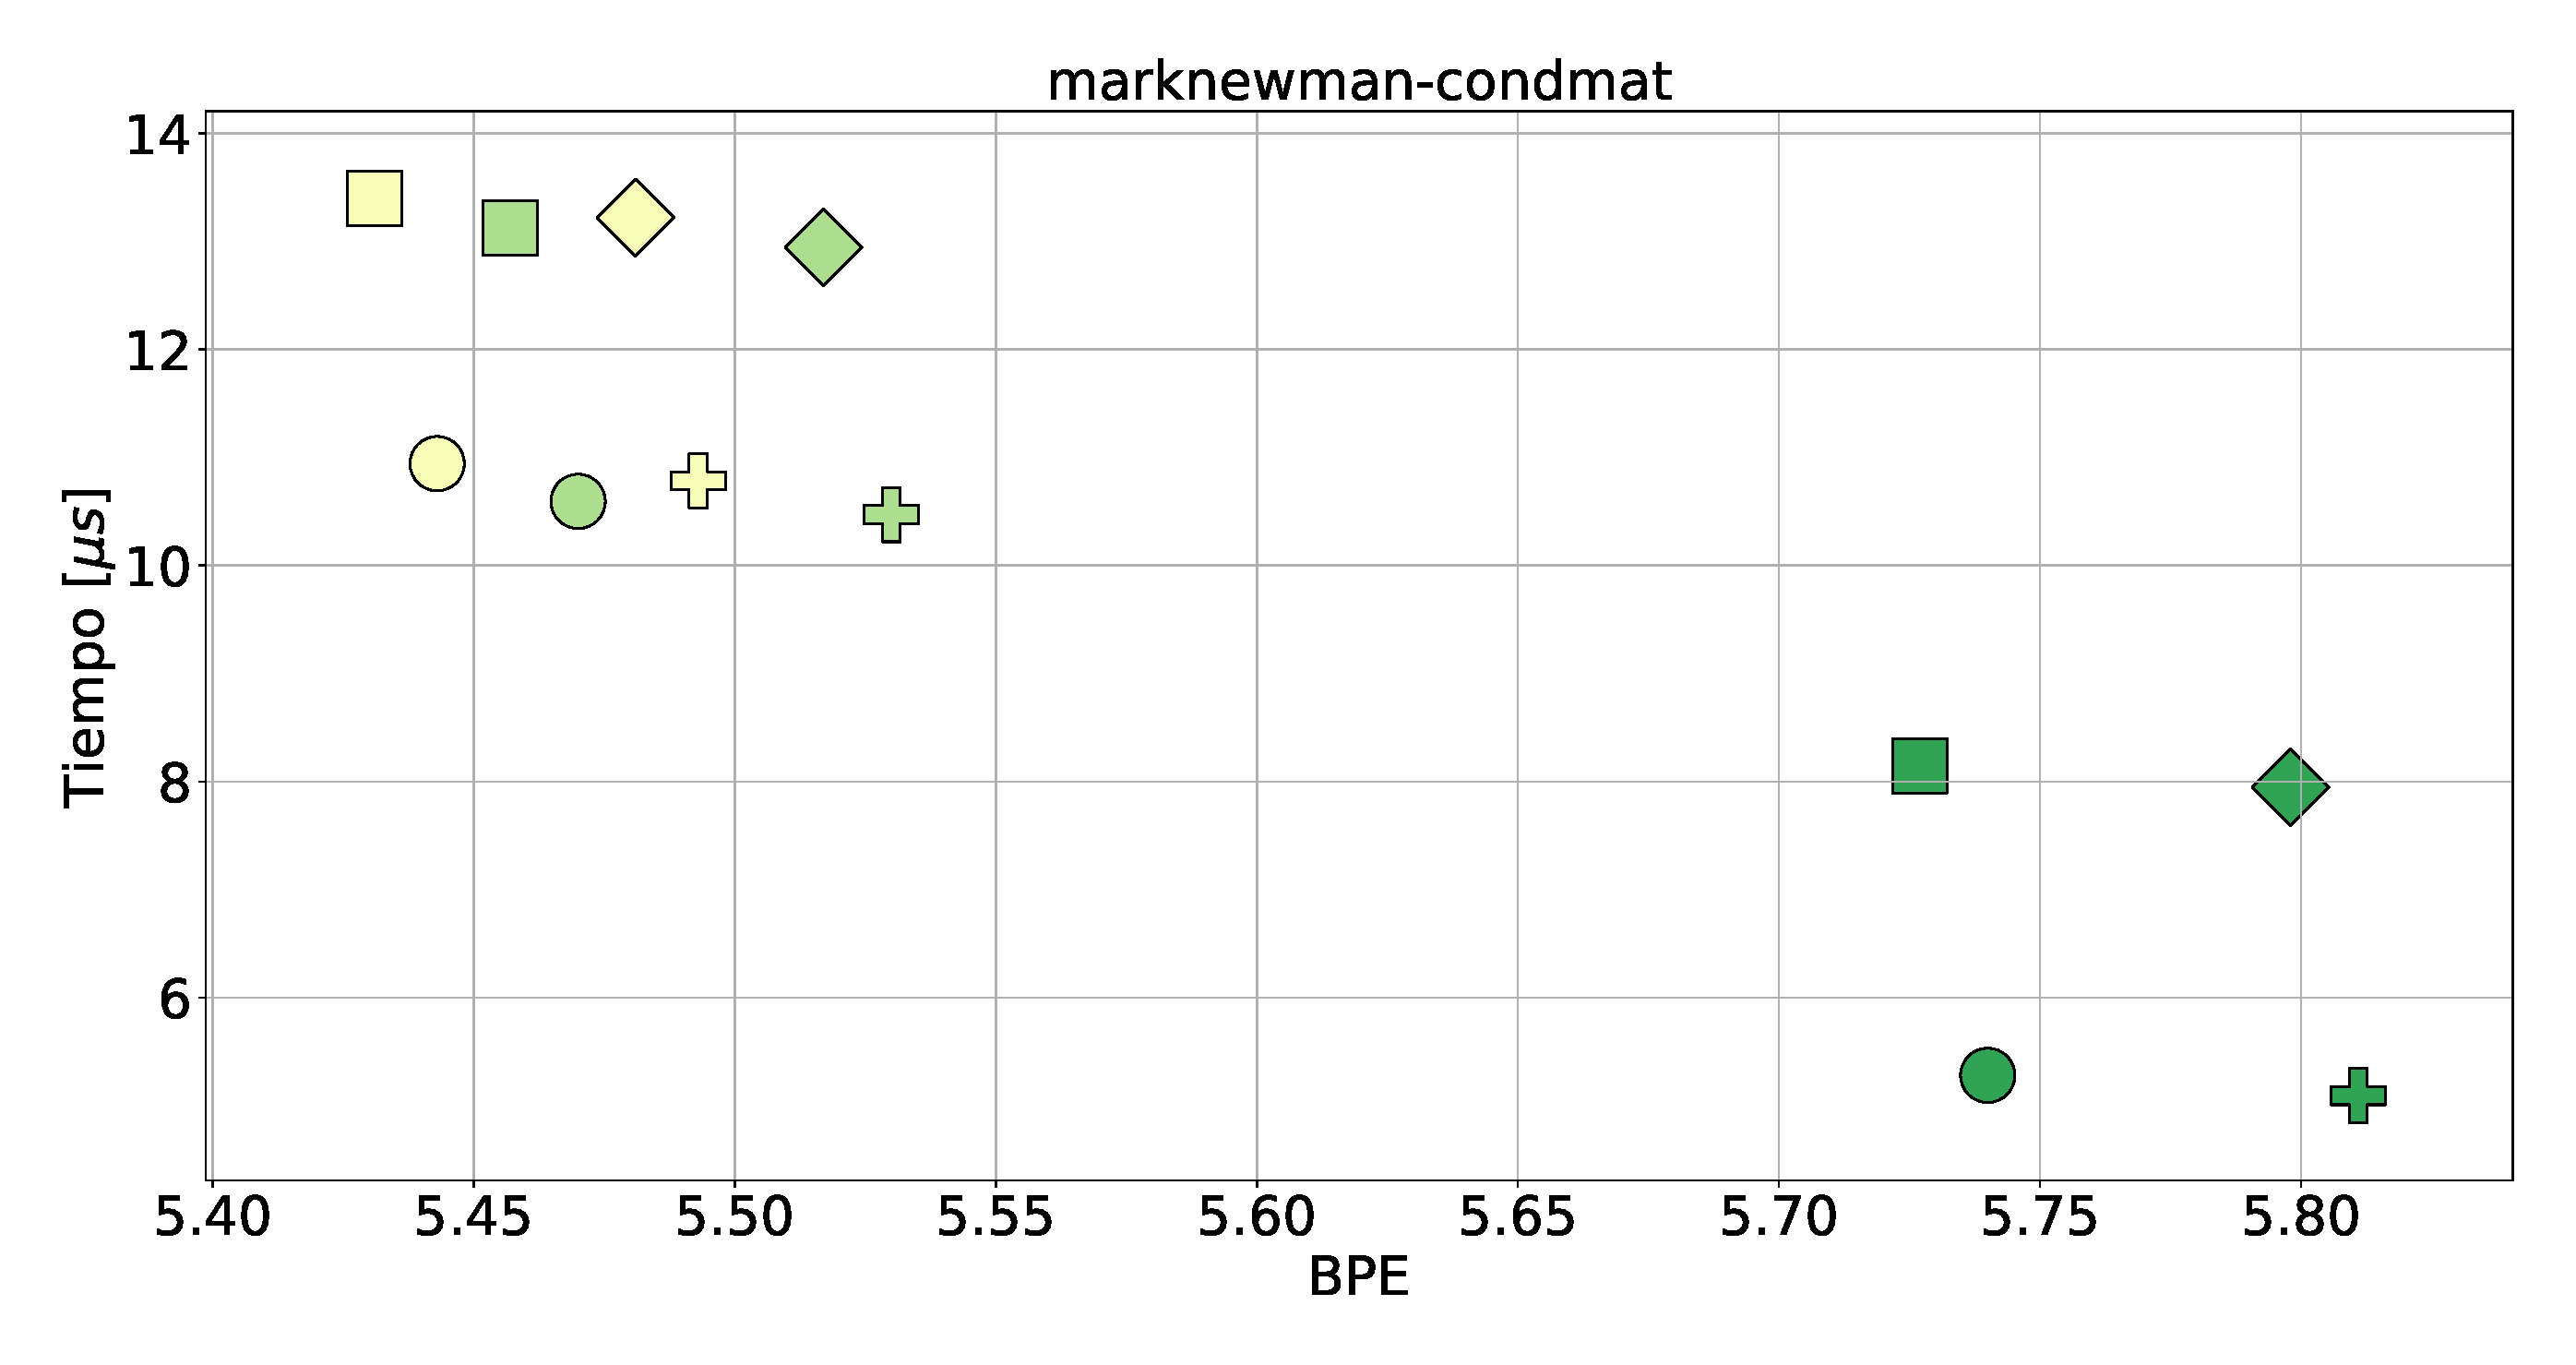
\includegraphics[width=1\linewidth]{img/sdsl/aleatorioBig/marknewman-condmat.pdf}
    			\end{minipage}
    			\begin{minipage}{0.15\textwidth}
    				\centering
    				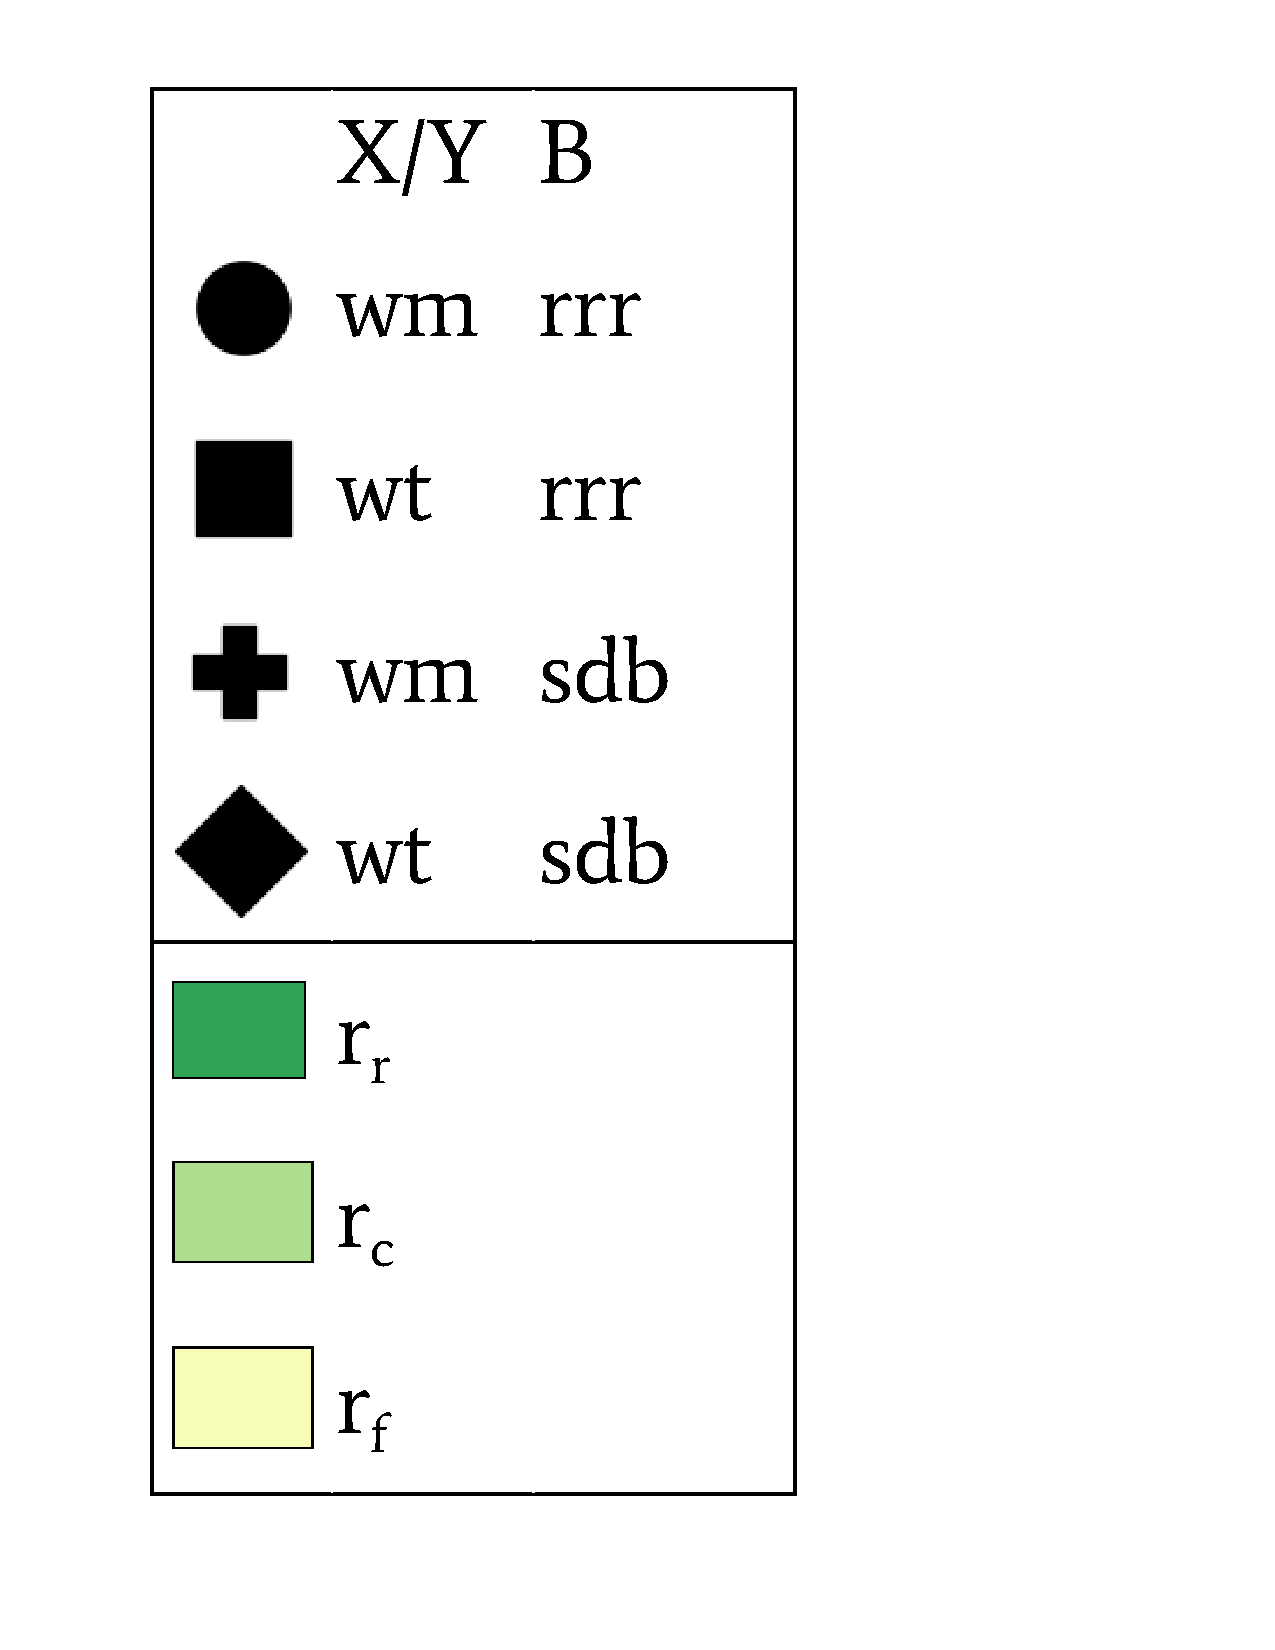
\includegraphics[scale=.22, clip, trim=70 0 0 0]{img/sdsl/label.pdf}
    			\end{minipage}
    			
    			(b)		
    	\end{minipage}
    	
    \caption{BPE y Tiempo de acceso aleatorio medio para posibles estructuras compactas, por cada función de ranking, para los grafos marknewman-astro y marknewman-condmat.}
    \label{fig:sdslBPEAle2}
\end{figure}

\begin{figure}
    	\centering
    	\begin{minipage}{1\textwidth}
    			\centering
    			\begin{minipage}{0.8\textwidth}
    				\centering
    				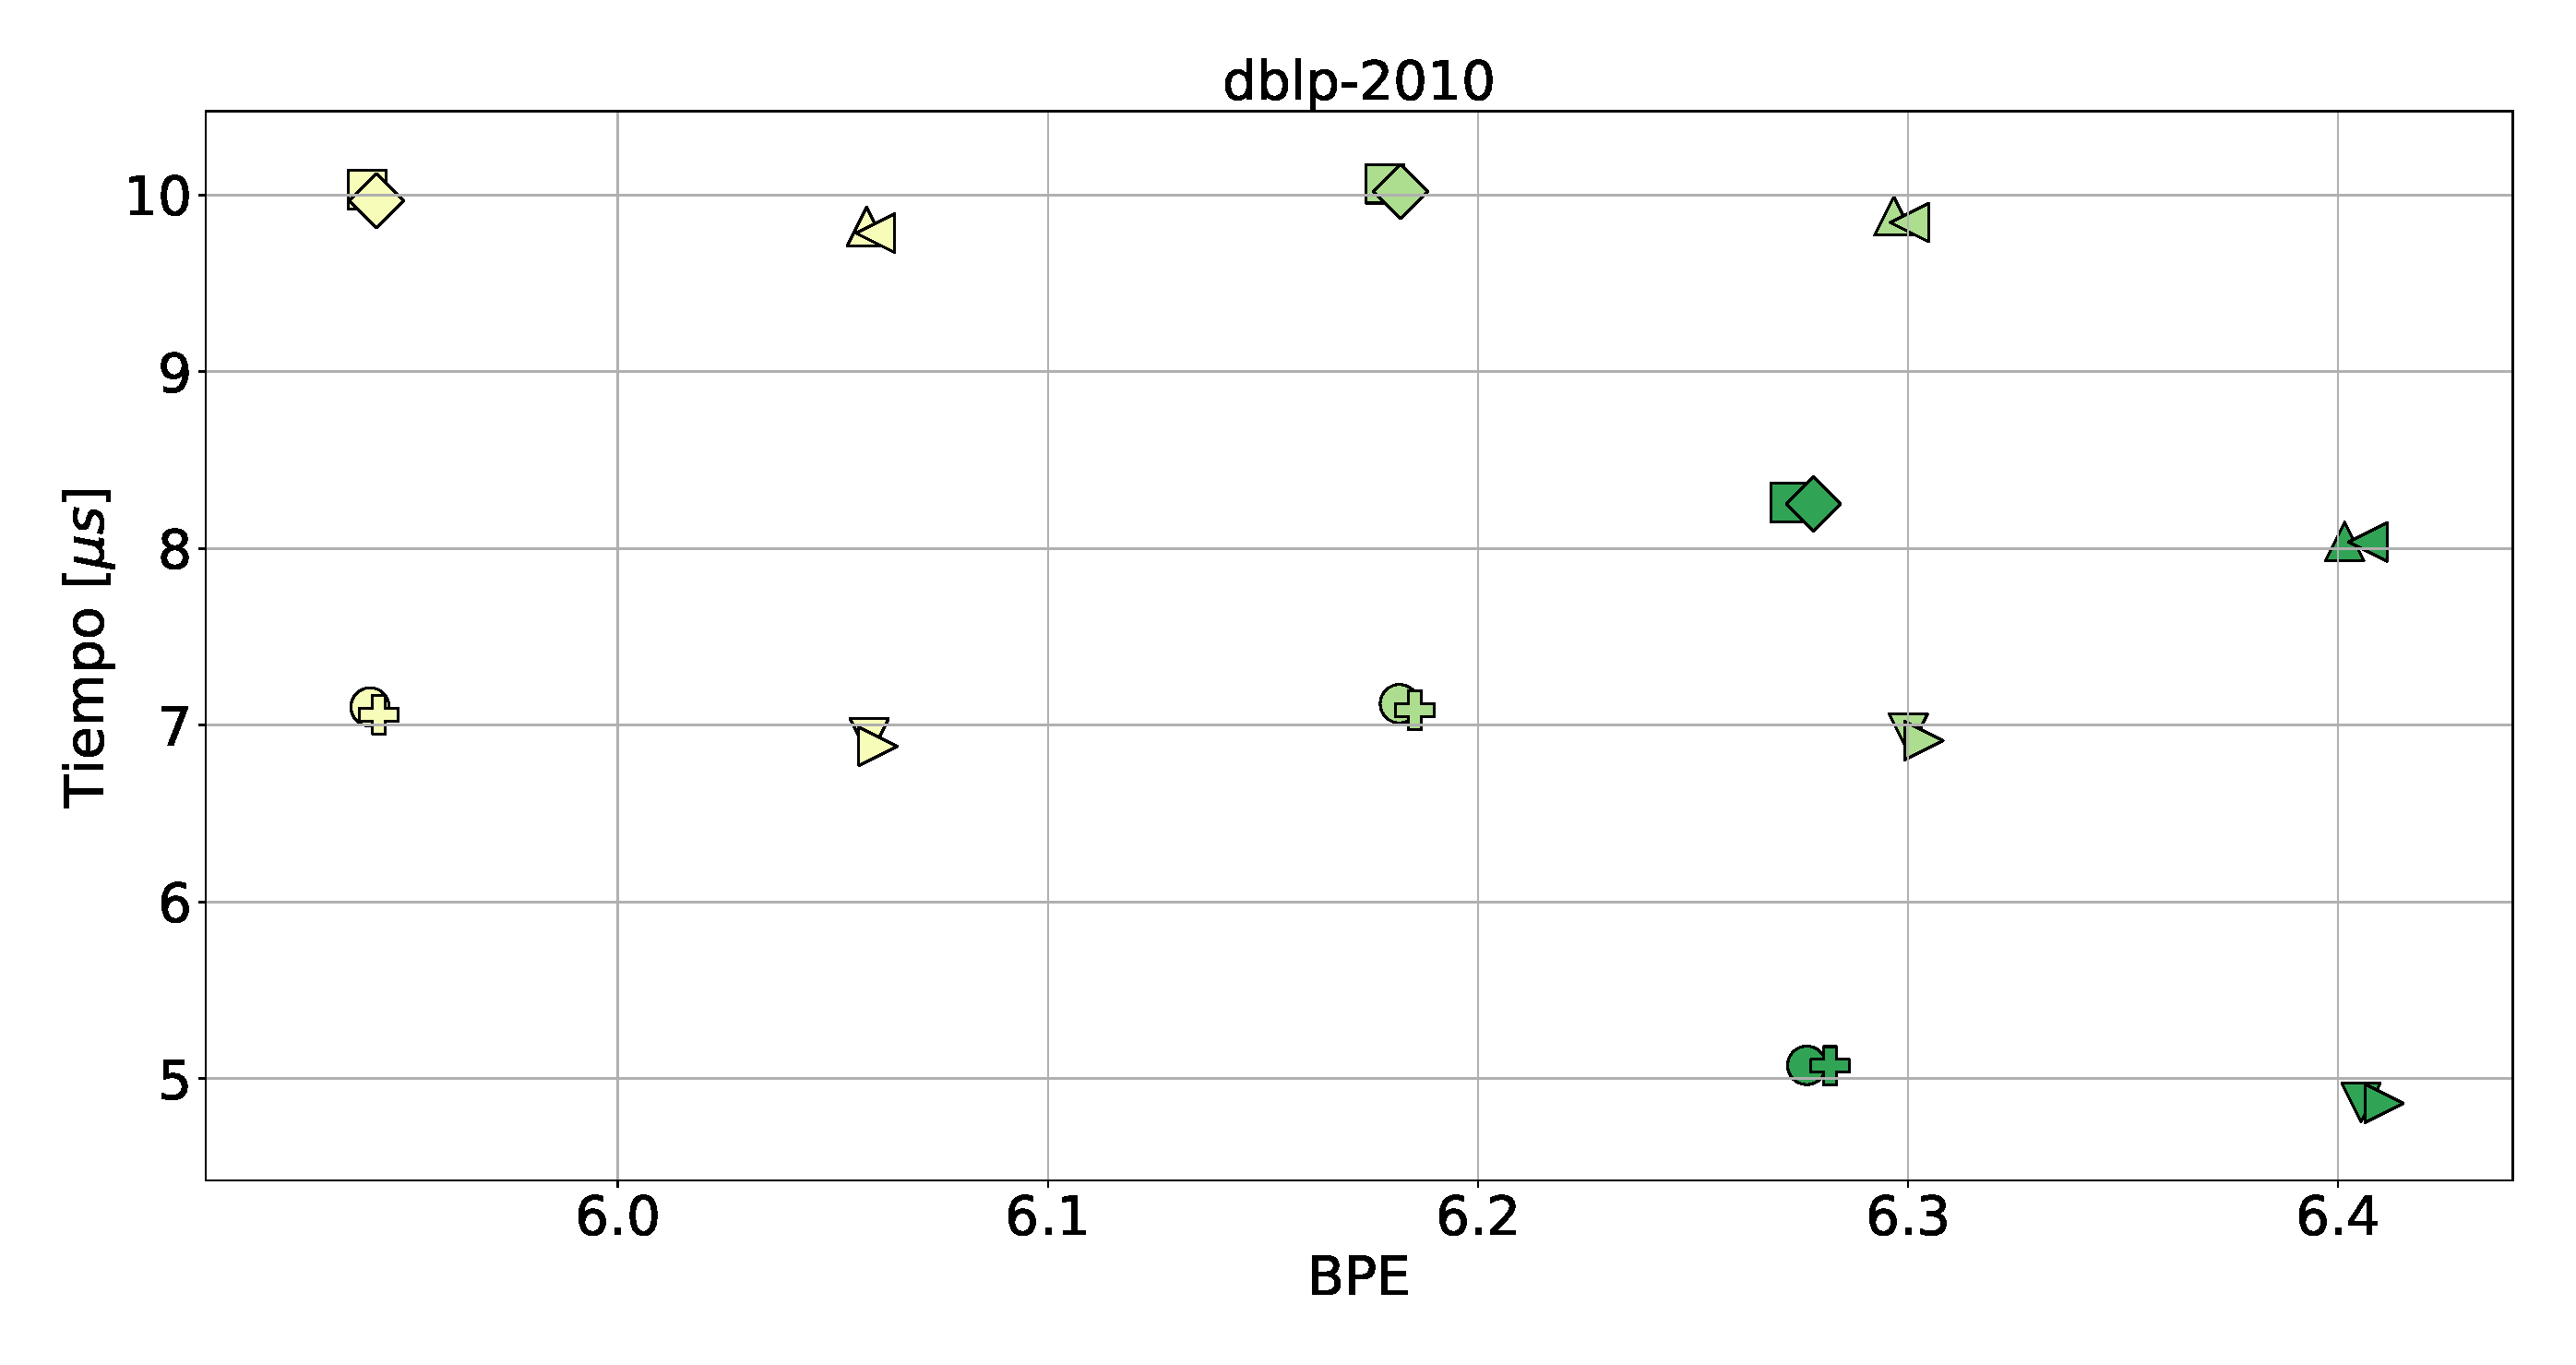
\includegraphics[width=1\linewidth]{img/sdsl/aleatorioBig/dblp-2010.pdf}
    			\end{minipage}
    			\begin{minipage}{0.15\textwidth}
    				\centering
    				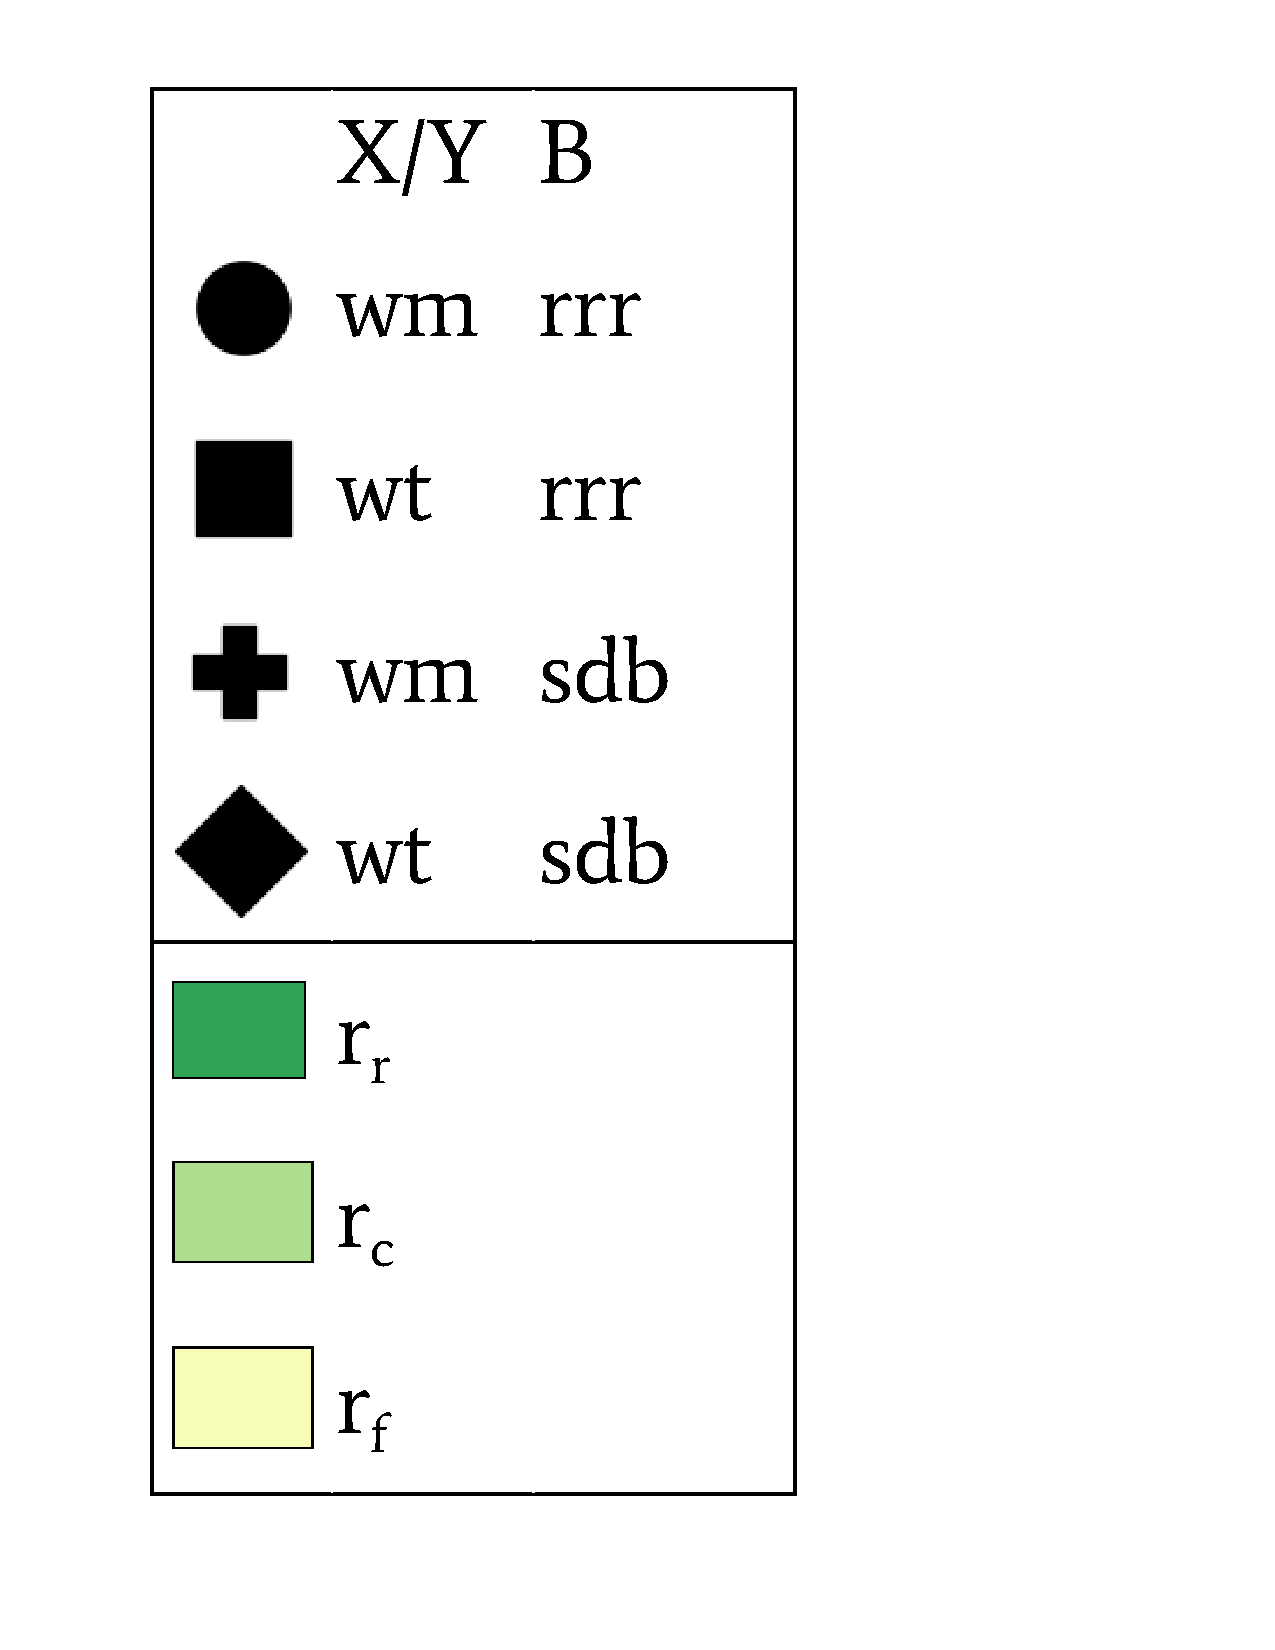
\includegraphics[scale=.235, clip, trim=70 0 0 0]{img/sdsl/label.pdf}
    			\end{minipage}
    			
    			(a)		
    	\end{minipage}
    	
       	\begin{minipage}{1\textwidth}
    			\centering
    			\begin{minipage}{0.8\textwidth}
    				\centering
    				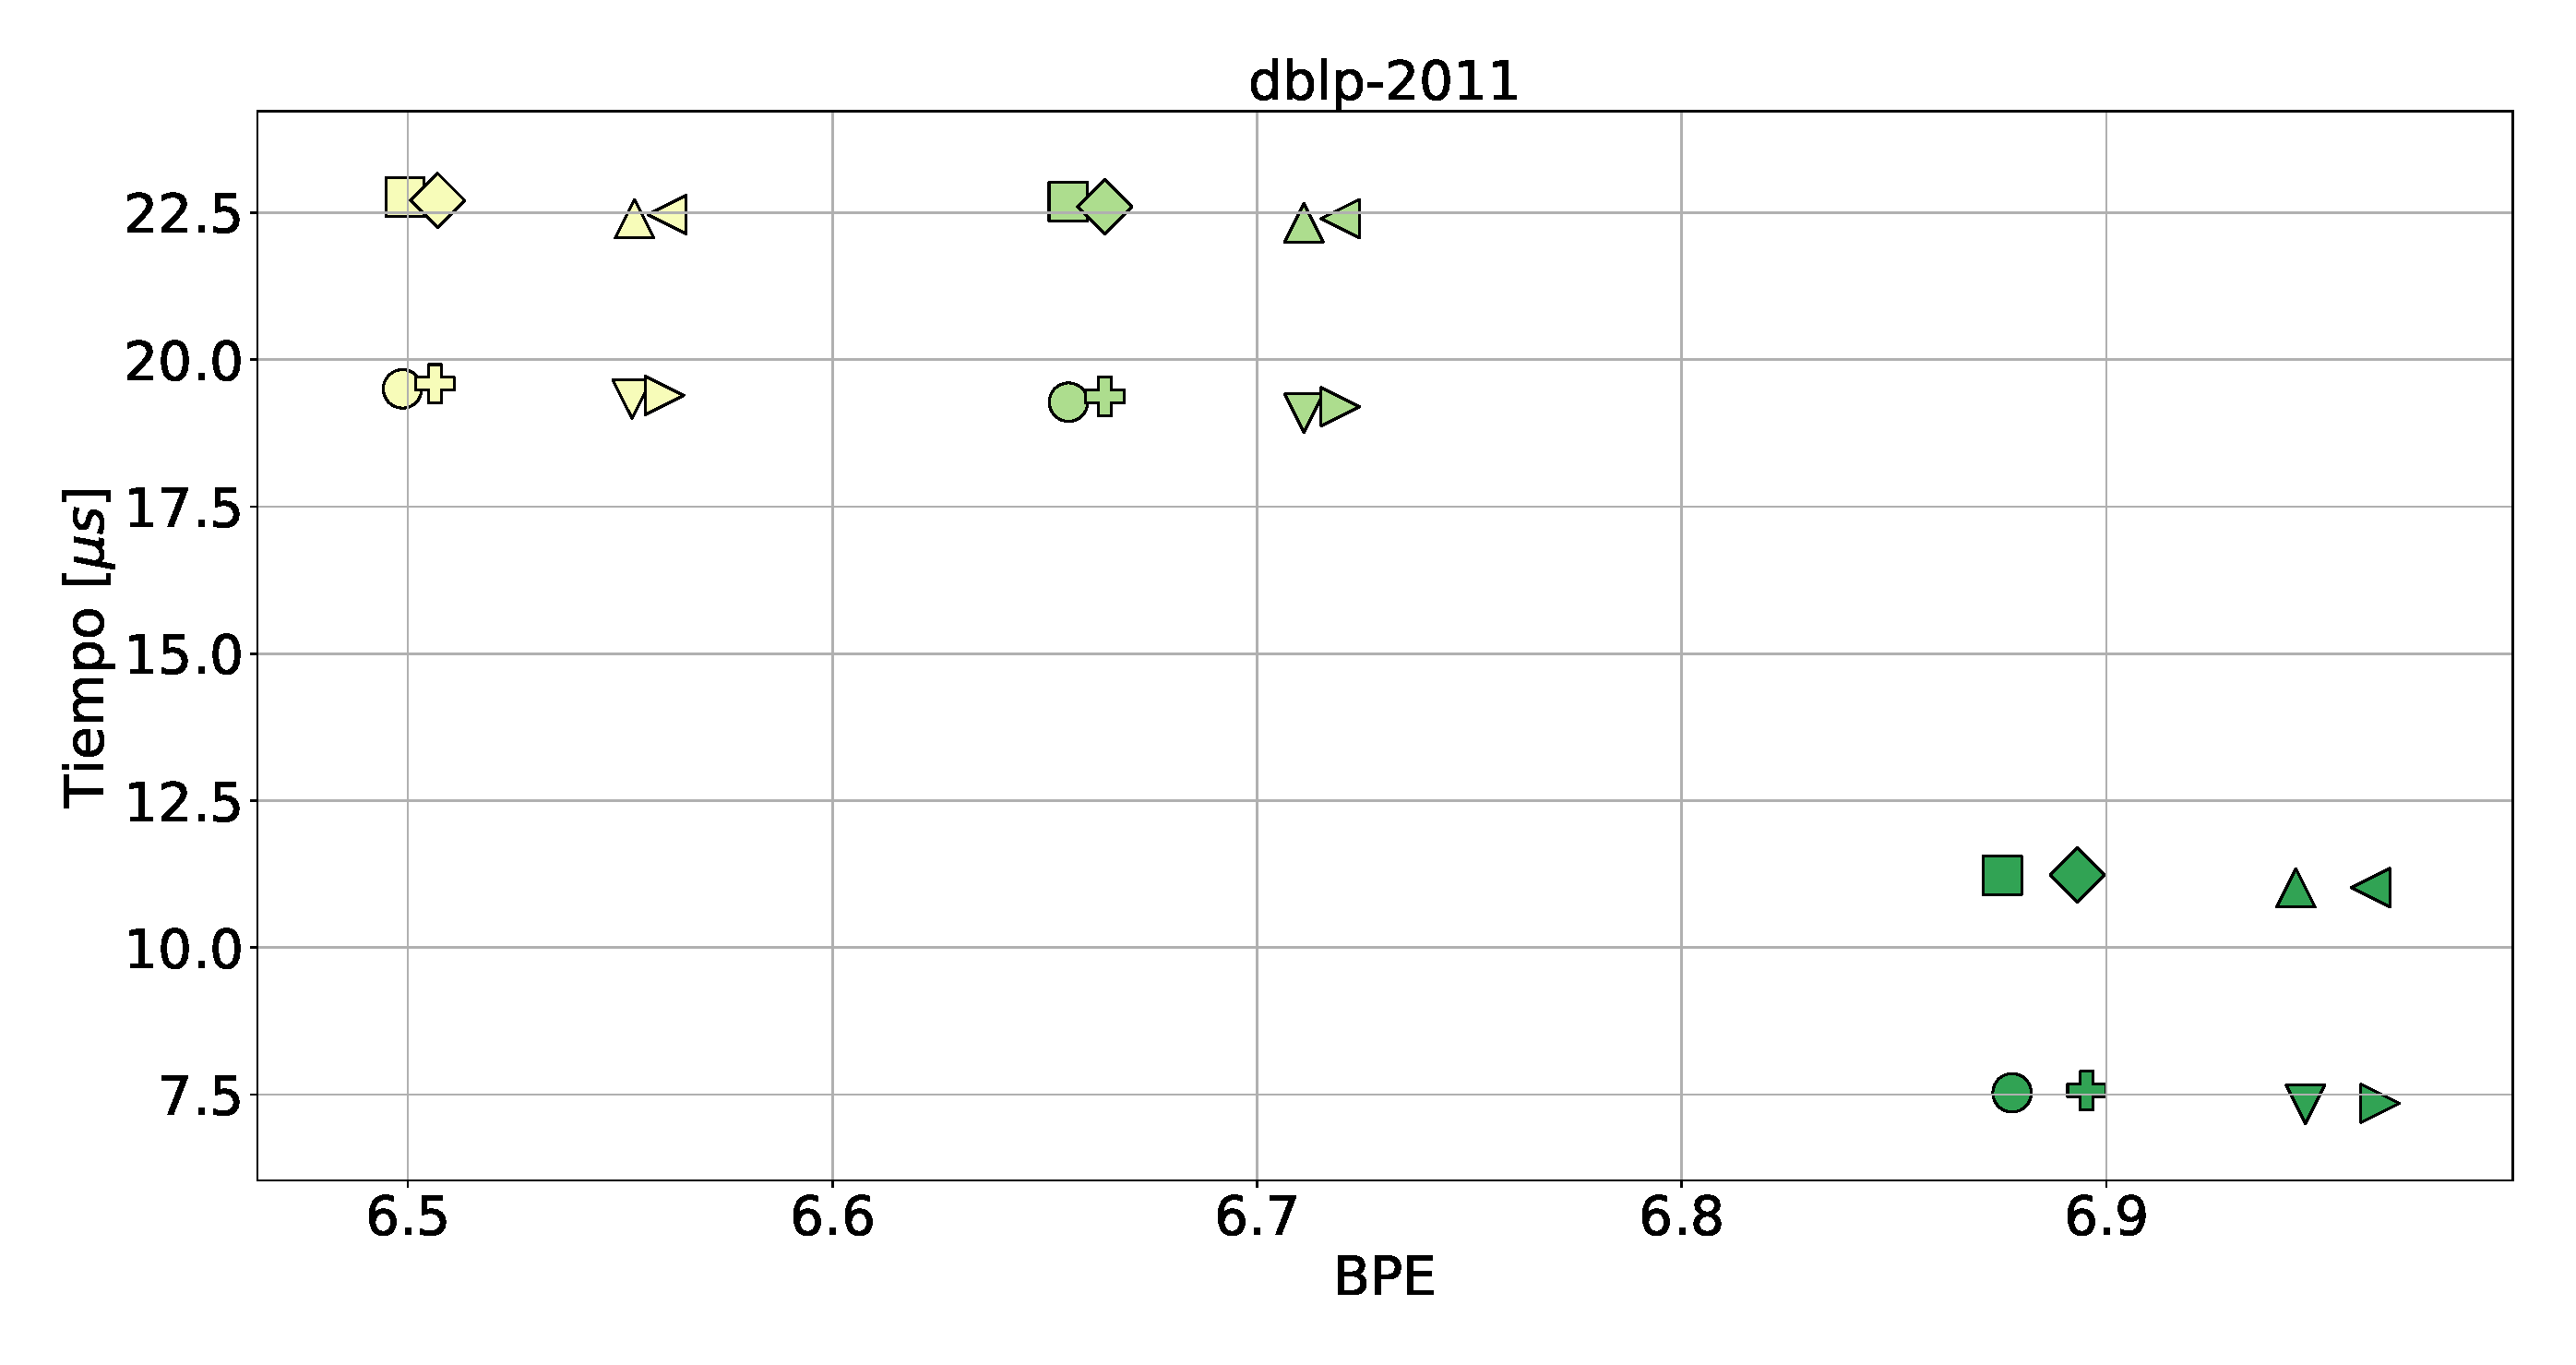
\includegraphics[width=1\linewidth]{img/sdsl/aleatorioBig/dblp-2011.pdf}
    			\end{minipage}
    			\begin{minipage}{0.15\textwidth}
    				\centering
    				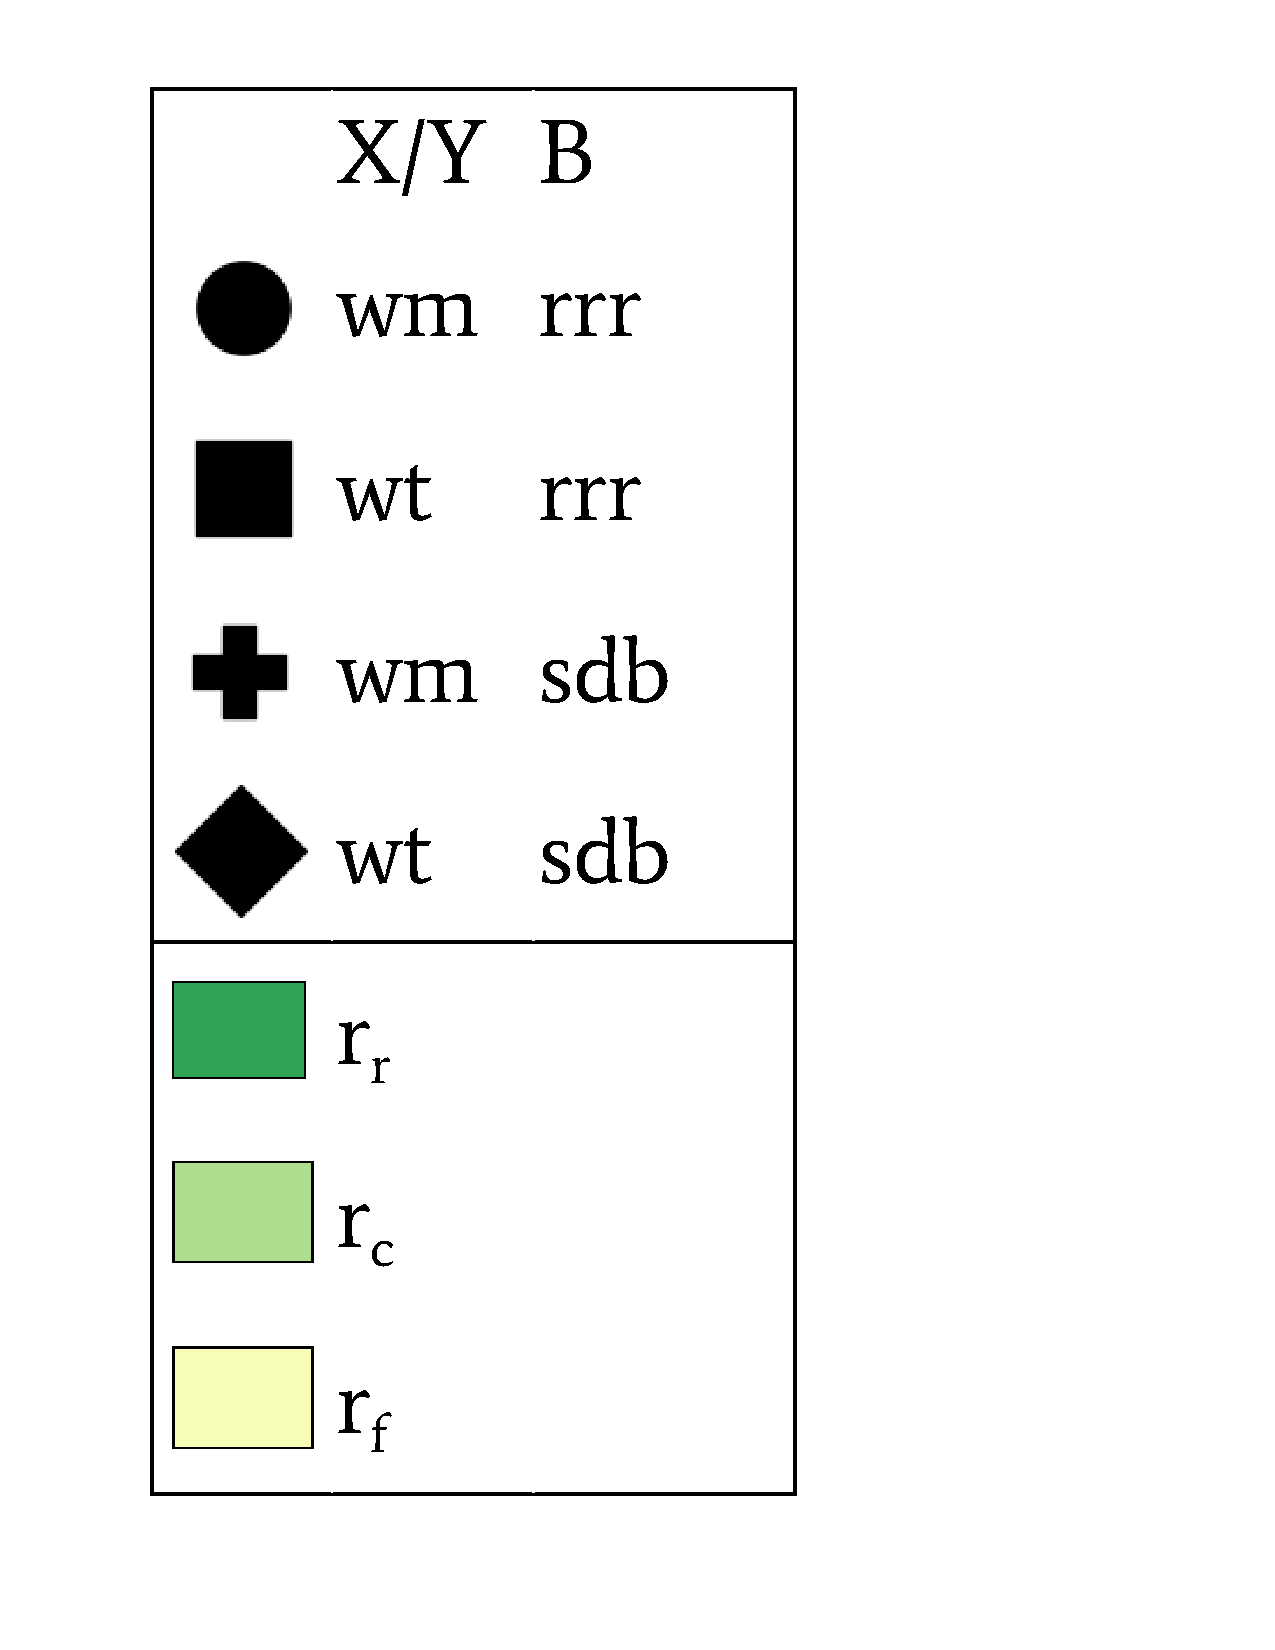
\includegraphics[scale=.235, clip, trim=70 0 0 0]{img/sdsl/label.pdf}
    			\end{minipage}
    			
    			(b)		
    	\end{minipage}
    	
    \caption{BPE y Tiempo de acceso aleatorio medio para posibles estructuras compactas, por cada función de ranking, para los grafos dblp-2010 y dblp-2011.}
    \label{fig:sdslBPEAle3}
\end{figure}

\begin{figure}
    	\centering
    	\begin{minipage}{1\textwidth}
    			\centering
    			\begin{minipage}{0.8\textwidth}
    				\centering
    				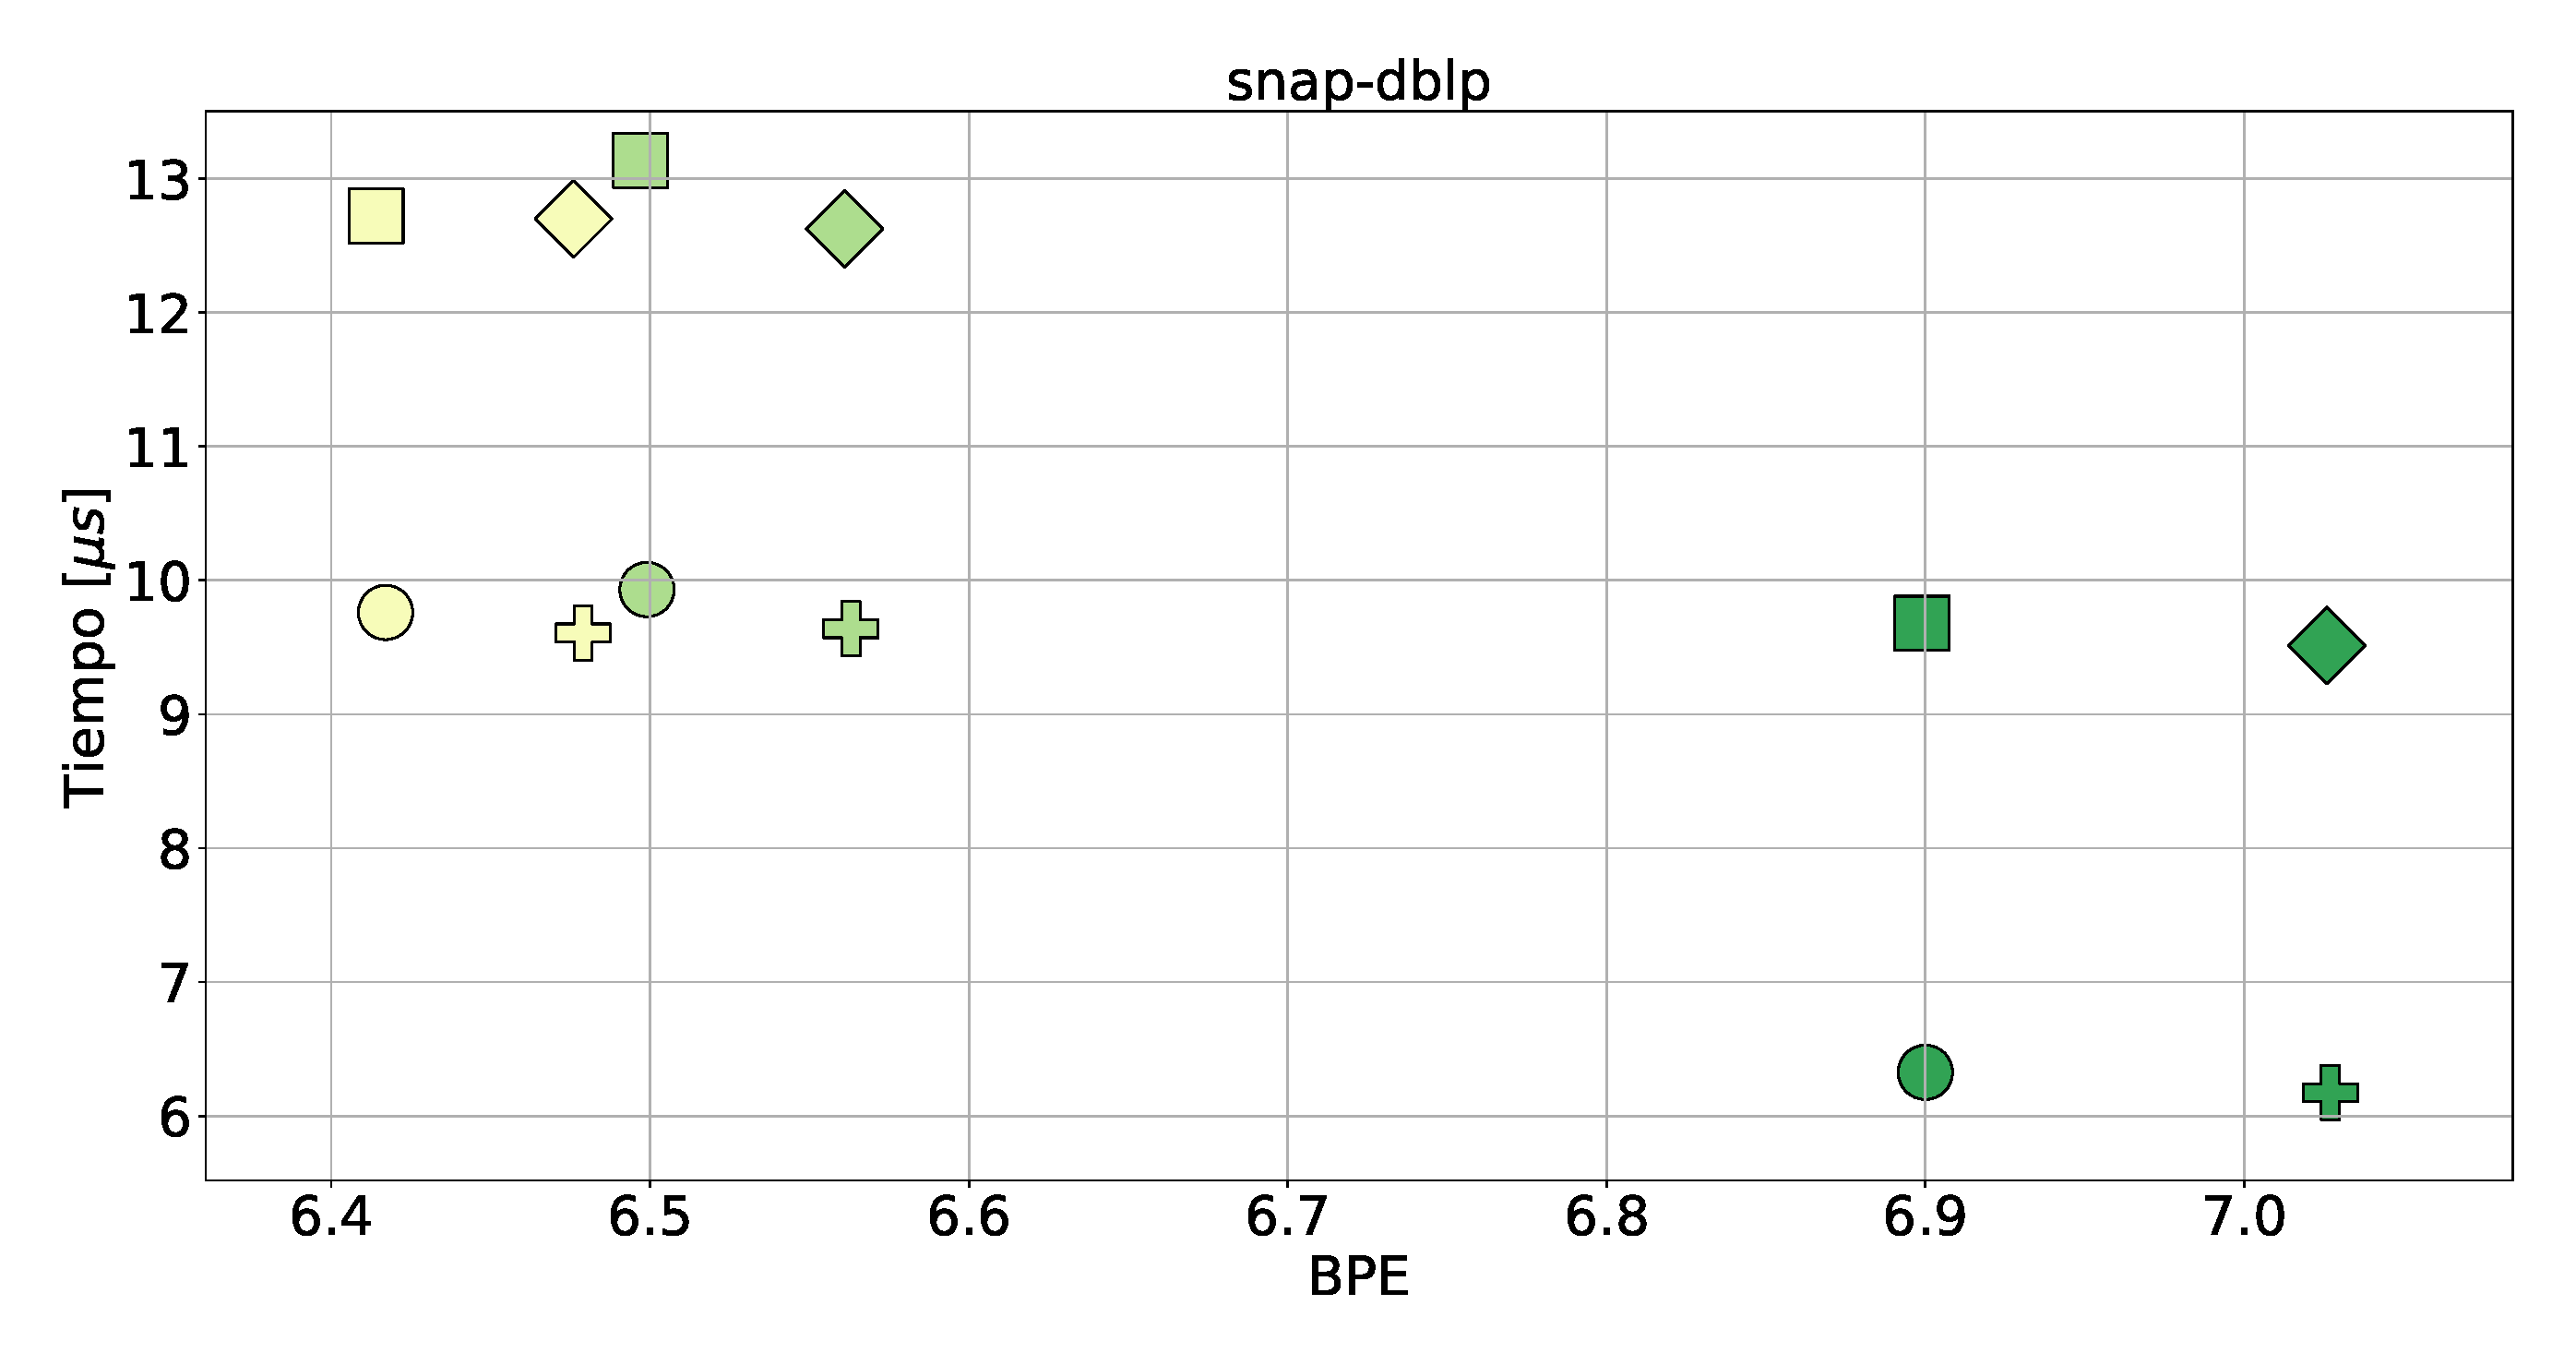
\includegraphics[width=1\linewidth]{img/sdsl/aleatorioBig/snap-dblp.pdf}
    			\end{minipage}
    			\begin{minipage}{0.15\textwidth}
    				\centering
    				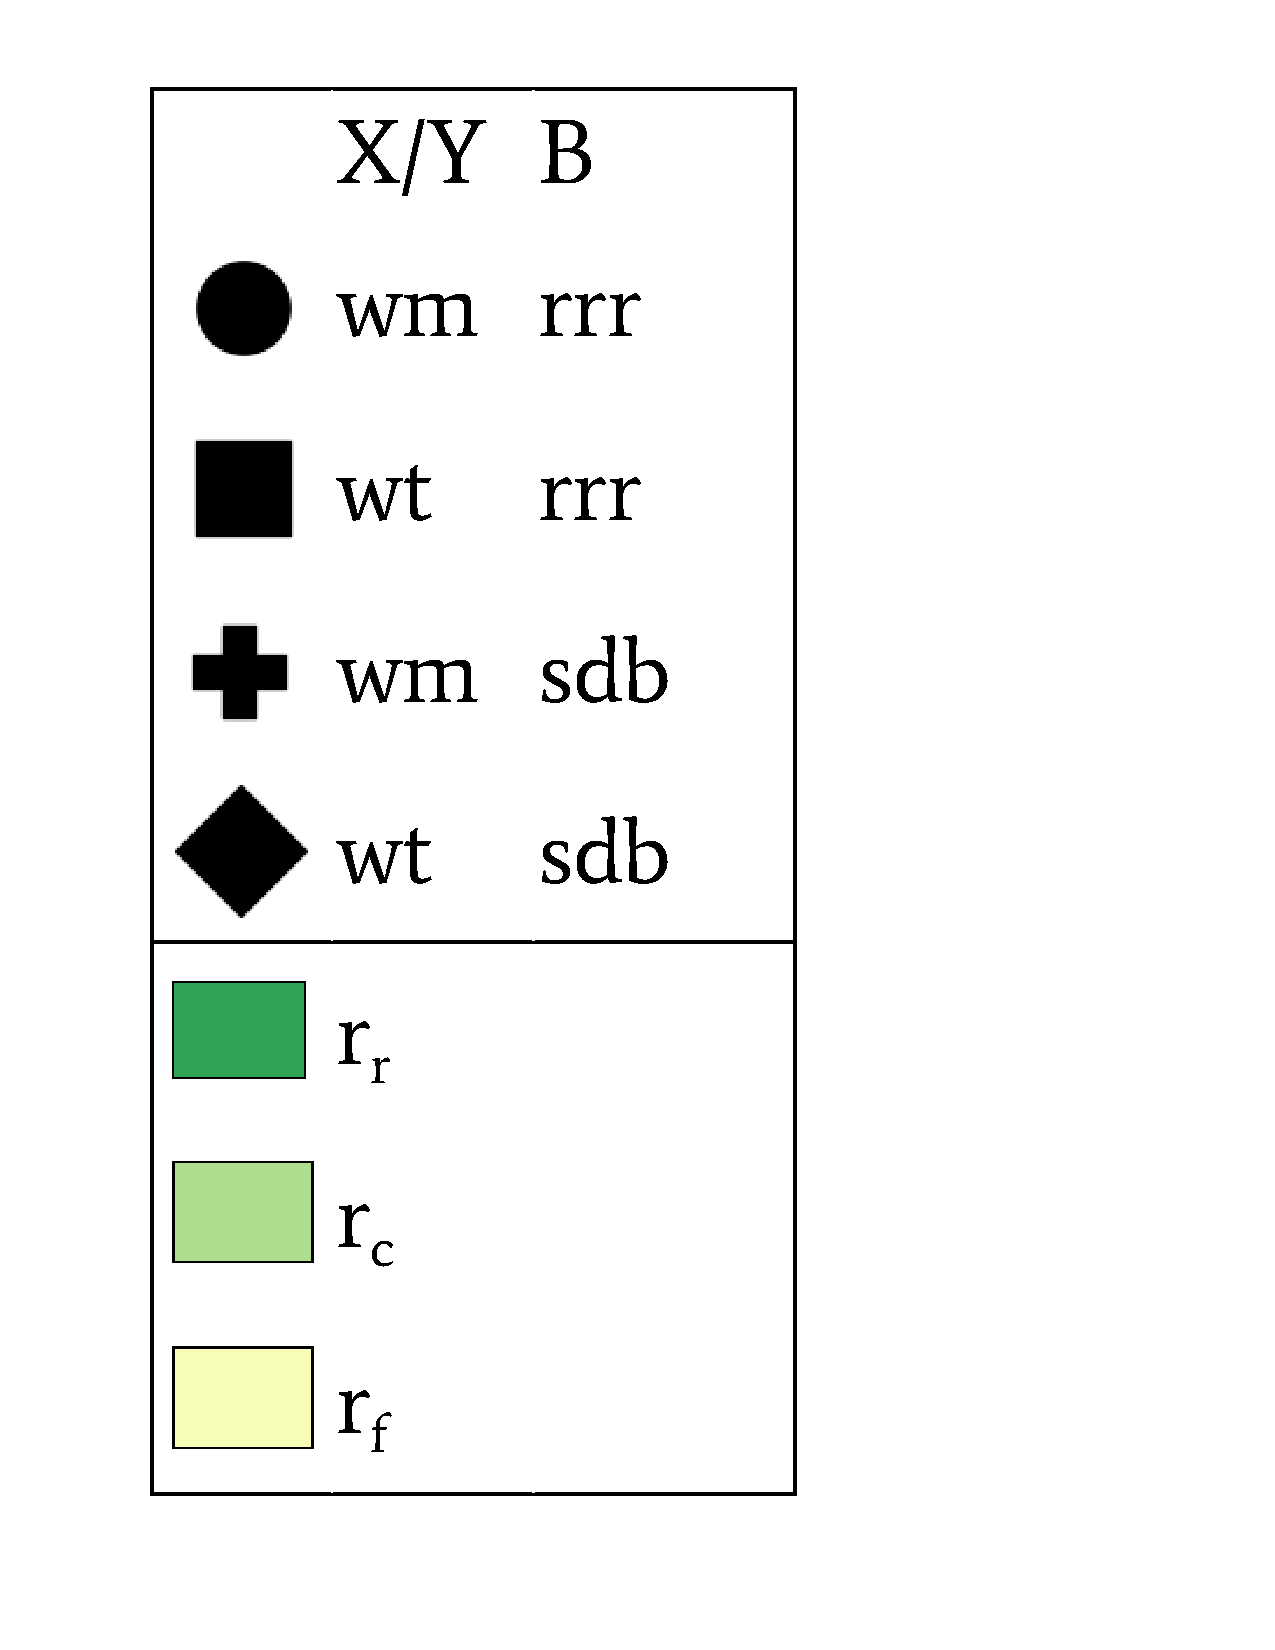
\includegraphics[scale=.22, clip, trim=70 0 0 0]{img/sdsl/label.pdf}
    			\end{minipage}
    			
    			(a)		
    	\end{minipage}
    	
       	\begin{minipage}{1\textwidth}
    			\centering
    			\begin{minipage}{0.8\textwidth}
    				\centering
    				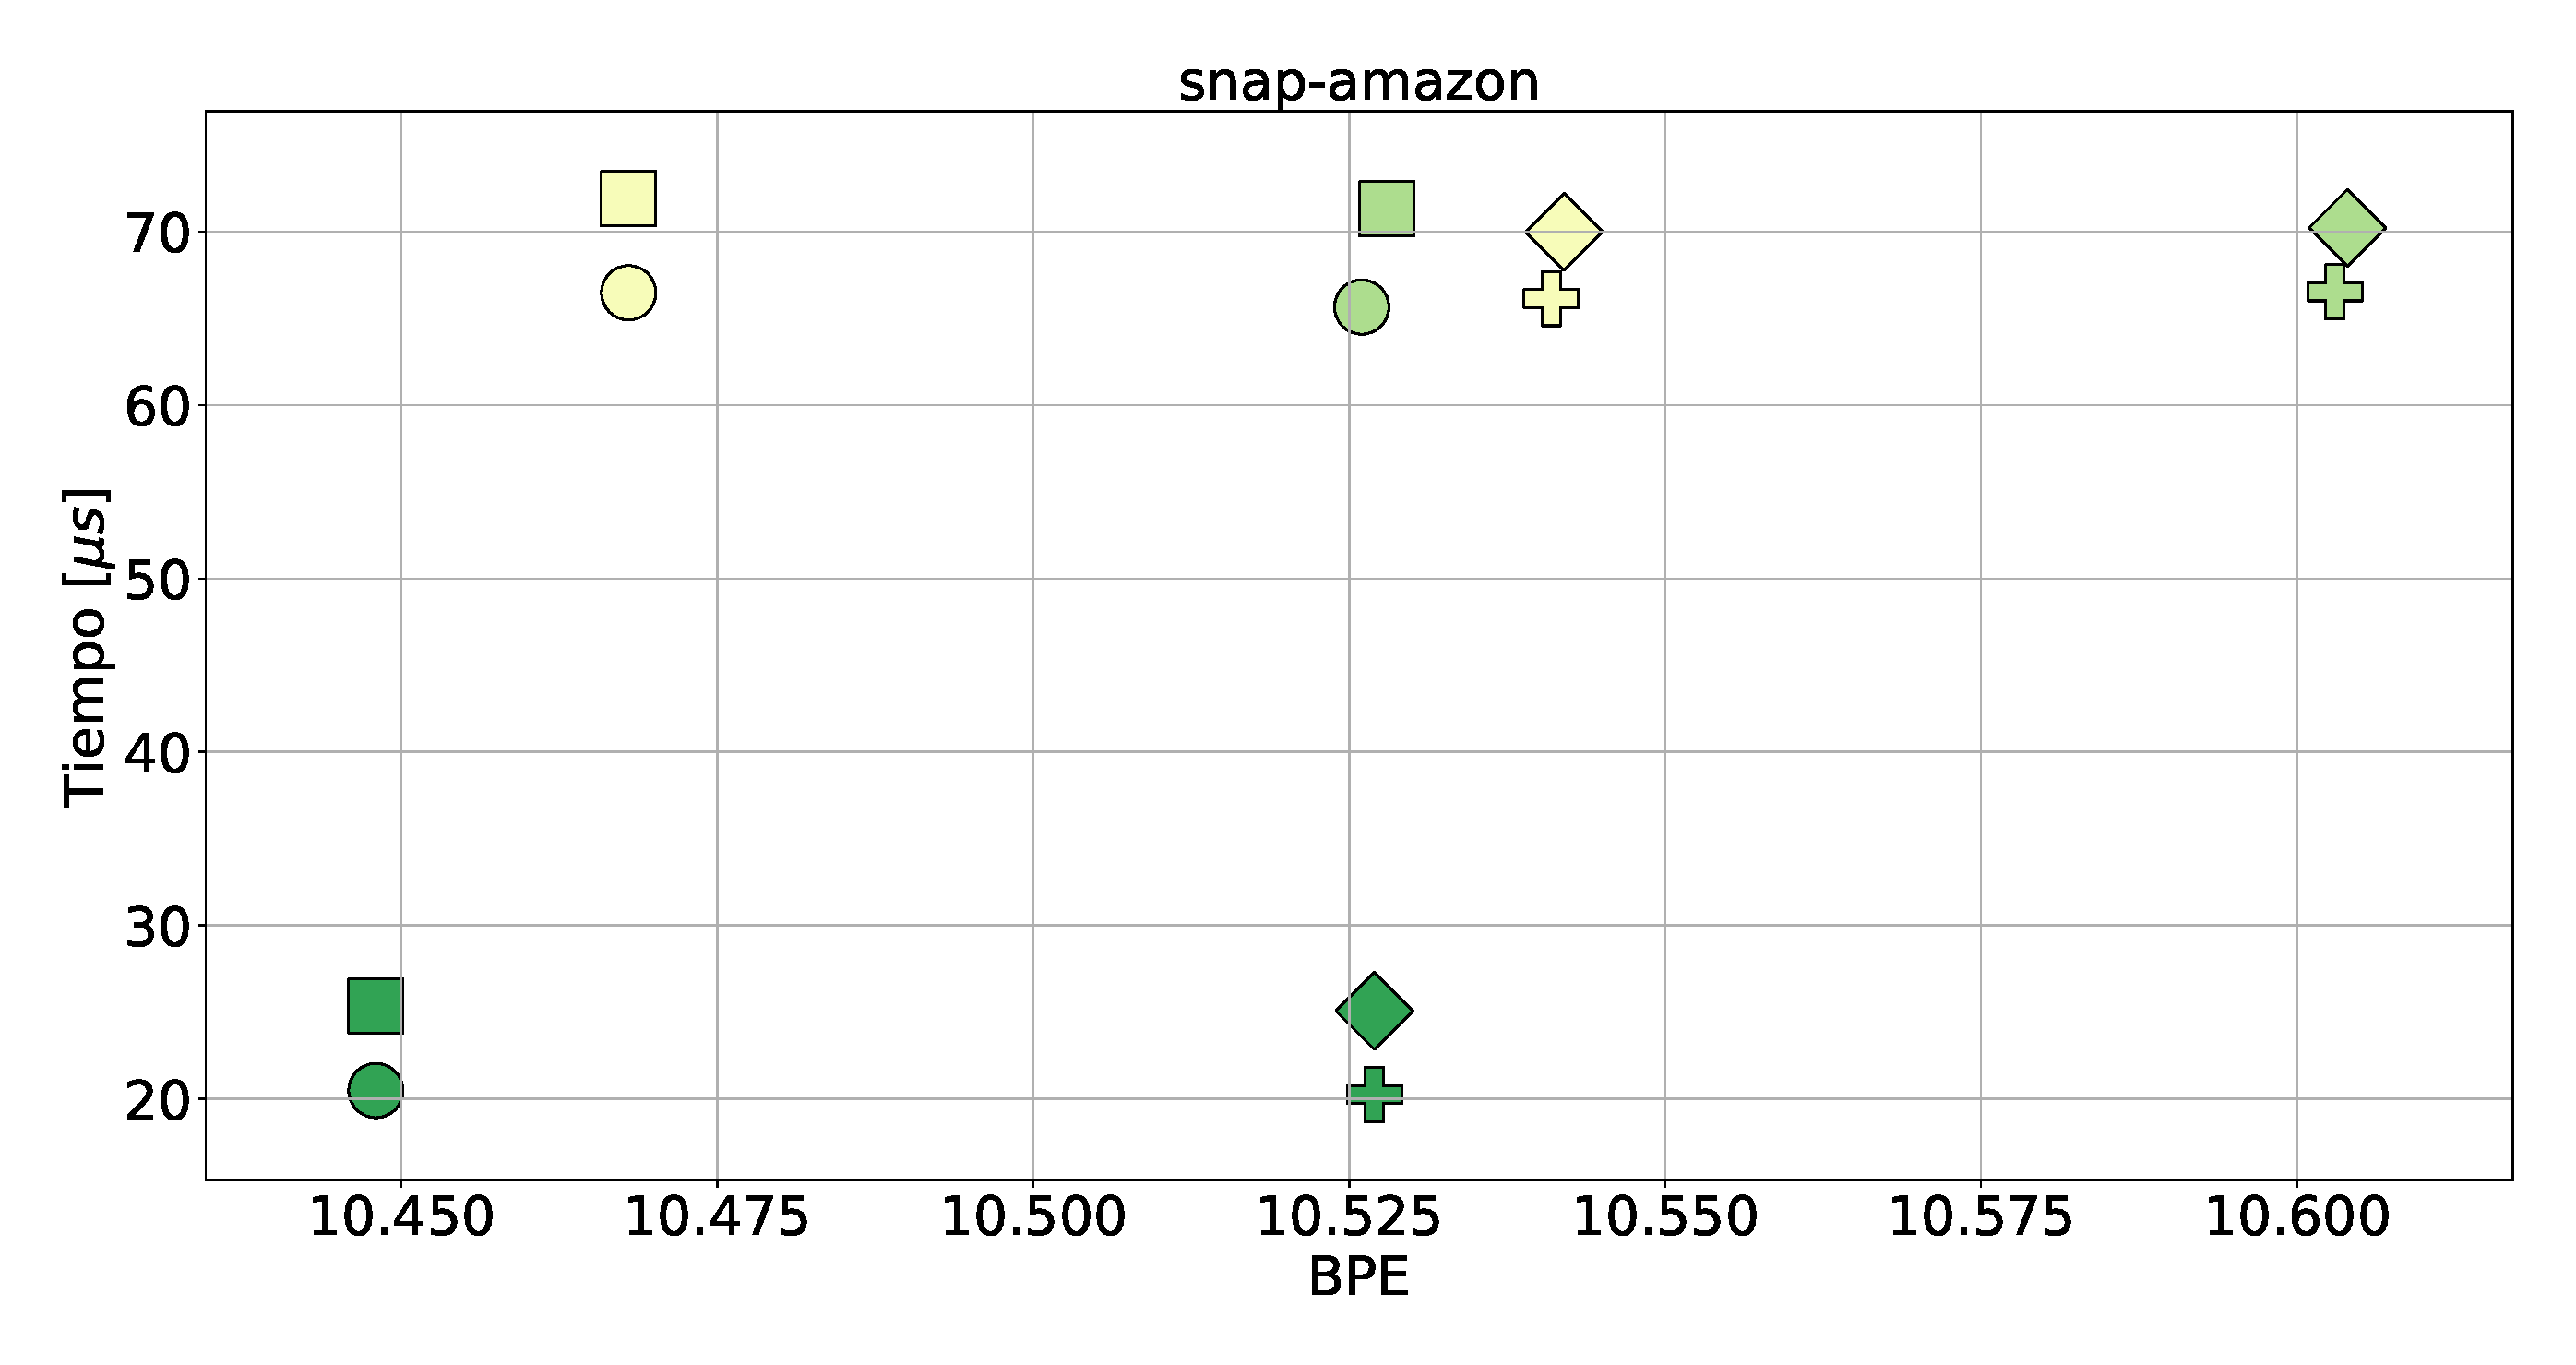
\includegraphics[width=1\linewidth]{img/sdsl/aleatorioBig/snap-amazon.pdf}
    			\end{minipage}
    			\begin{minipage}{0.15\textwidth}
    				\centering
    				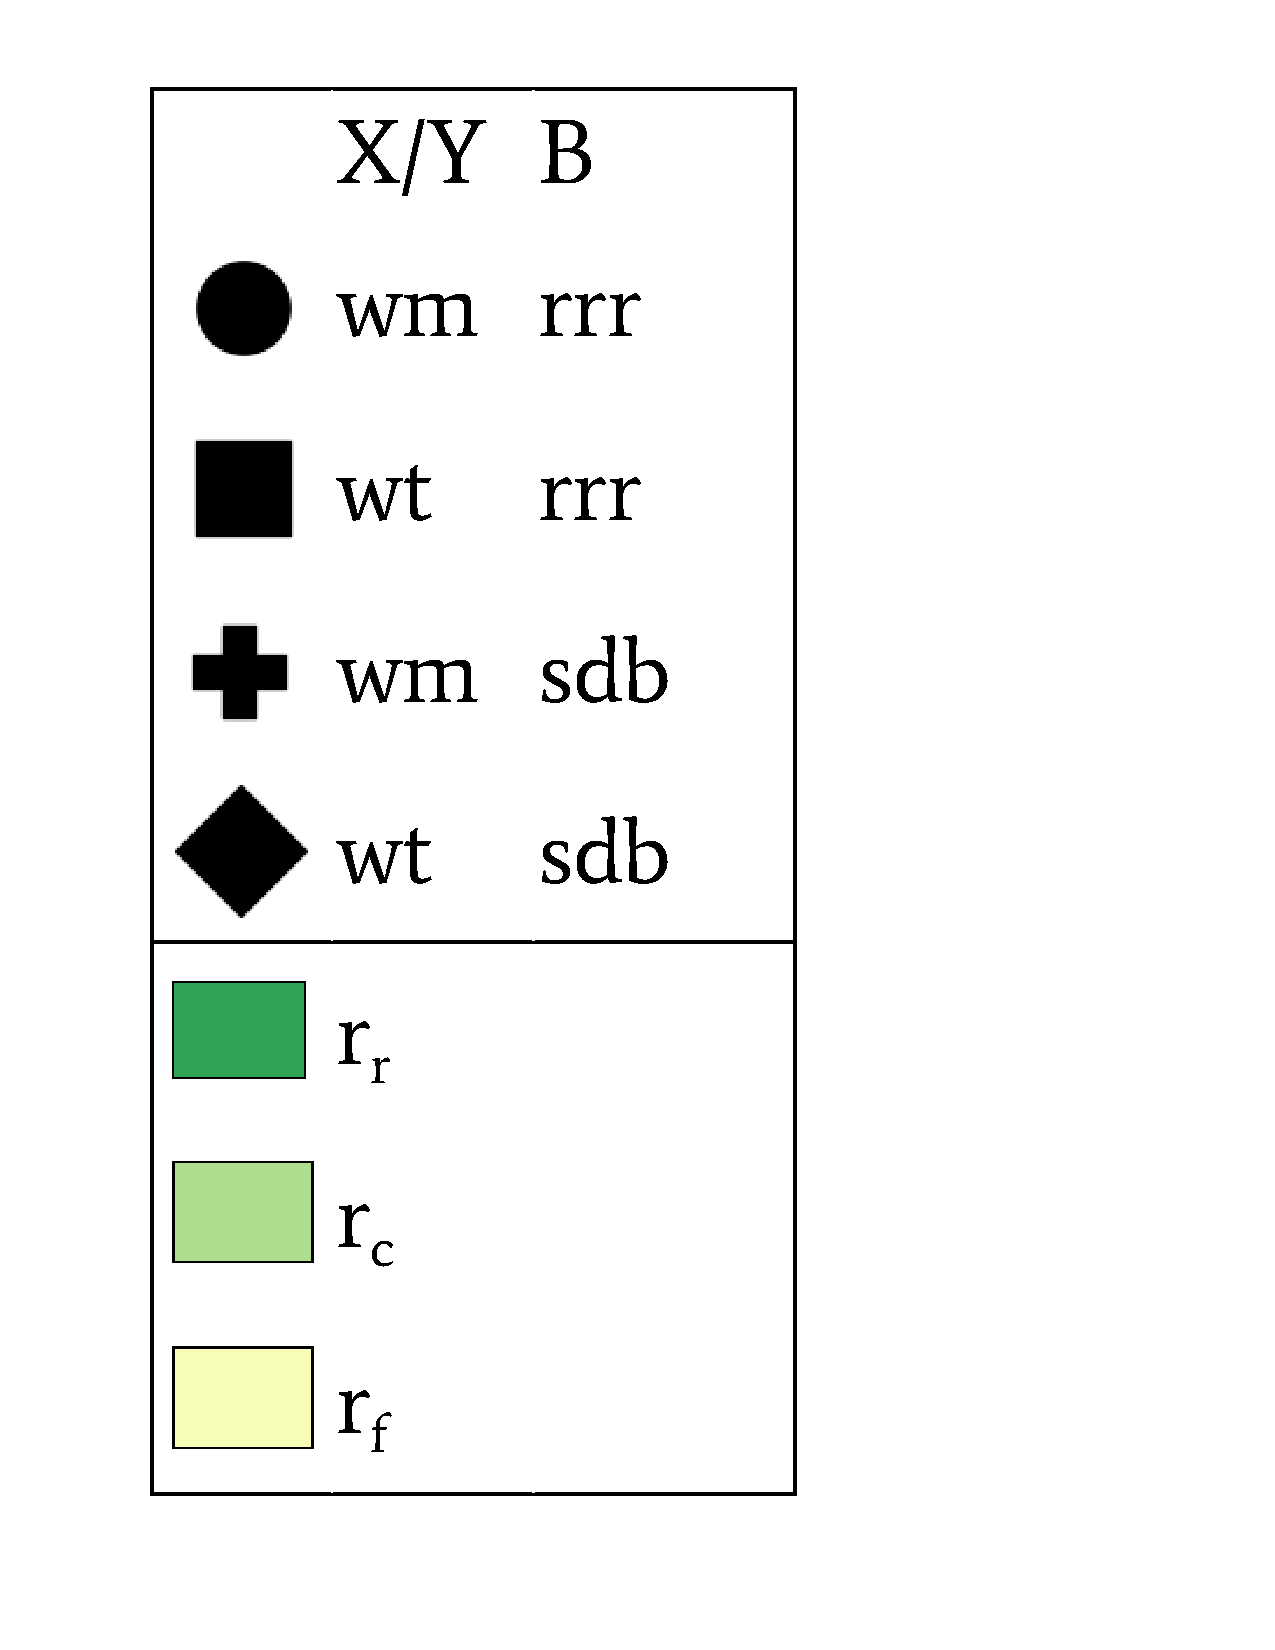
\includegraphics[scale=.22, clip, trim=70 0 0 0]{img/sdsl/label.pdf}
    			\end{minipage}
    			
    			(b)		
    	\end{minipage}
    	
    \caption{BPE y Tiempo de acceso aleatorio medio para posibles estructuras compactas, por cada función de ranking, para los grafos snap-dblp y snap-amazon.}
    \label{fig:sdslBPEAle4}
\end{figure}

\begin{figure}
    	\centering
    	\begin{minipage}{1\textwidth}
    			\centering
    			\begin{minipage}{0.8\textwidth}
    				\centering
    				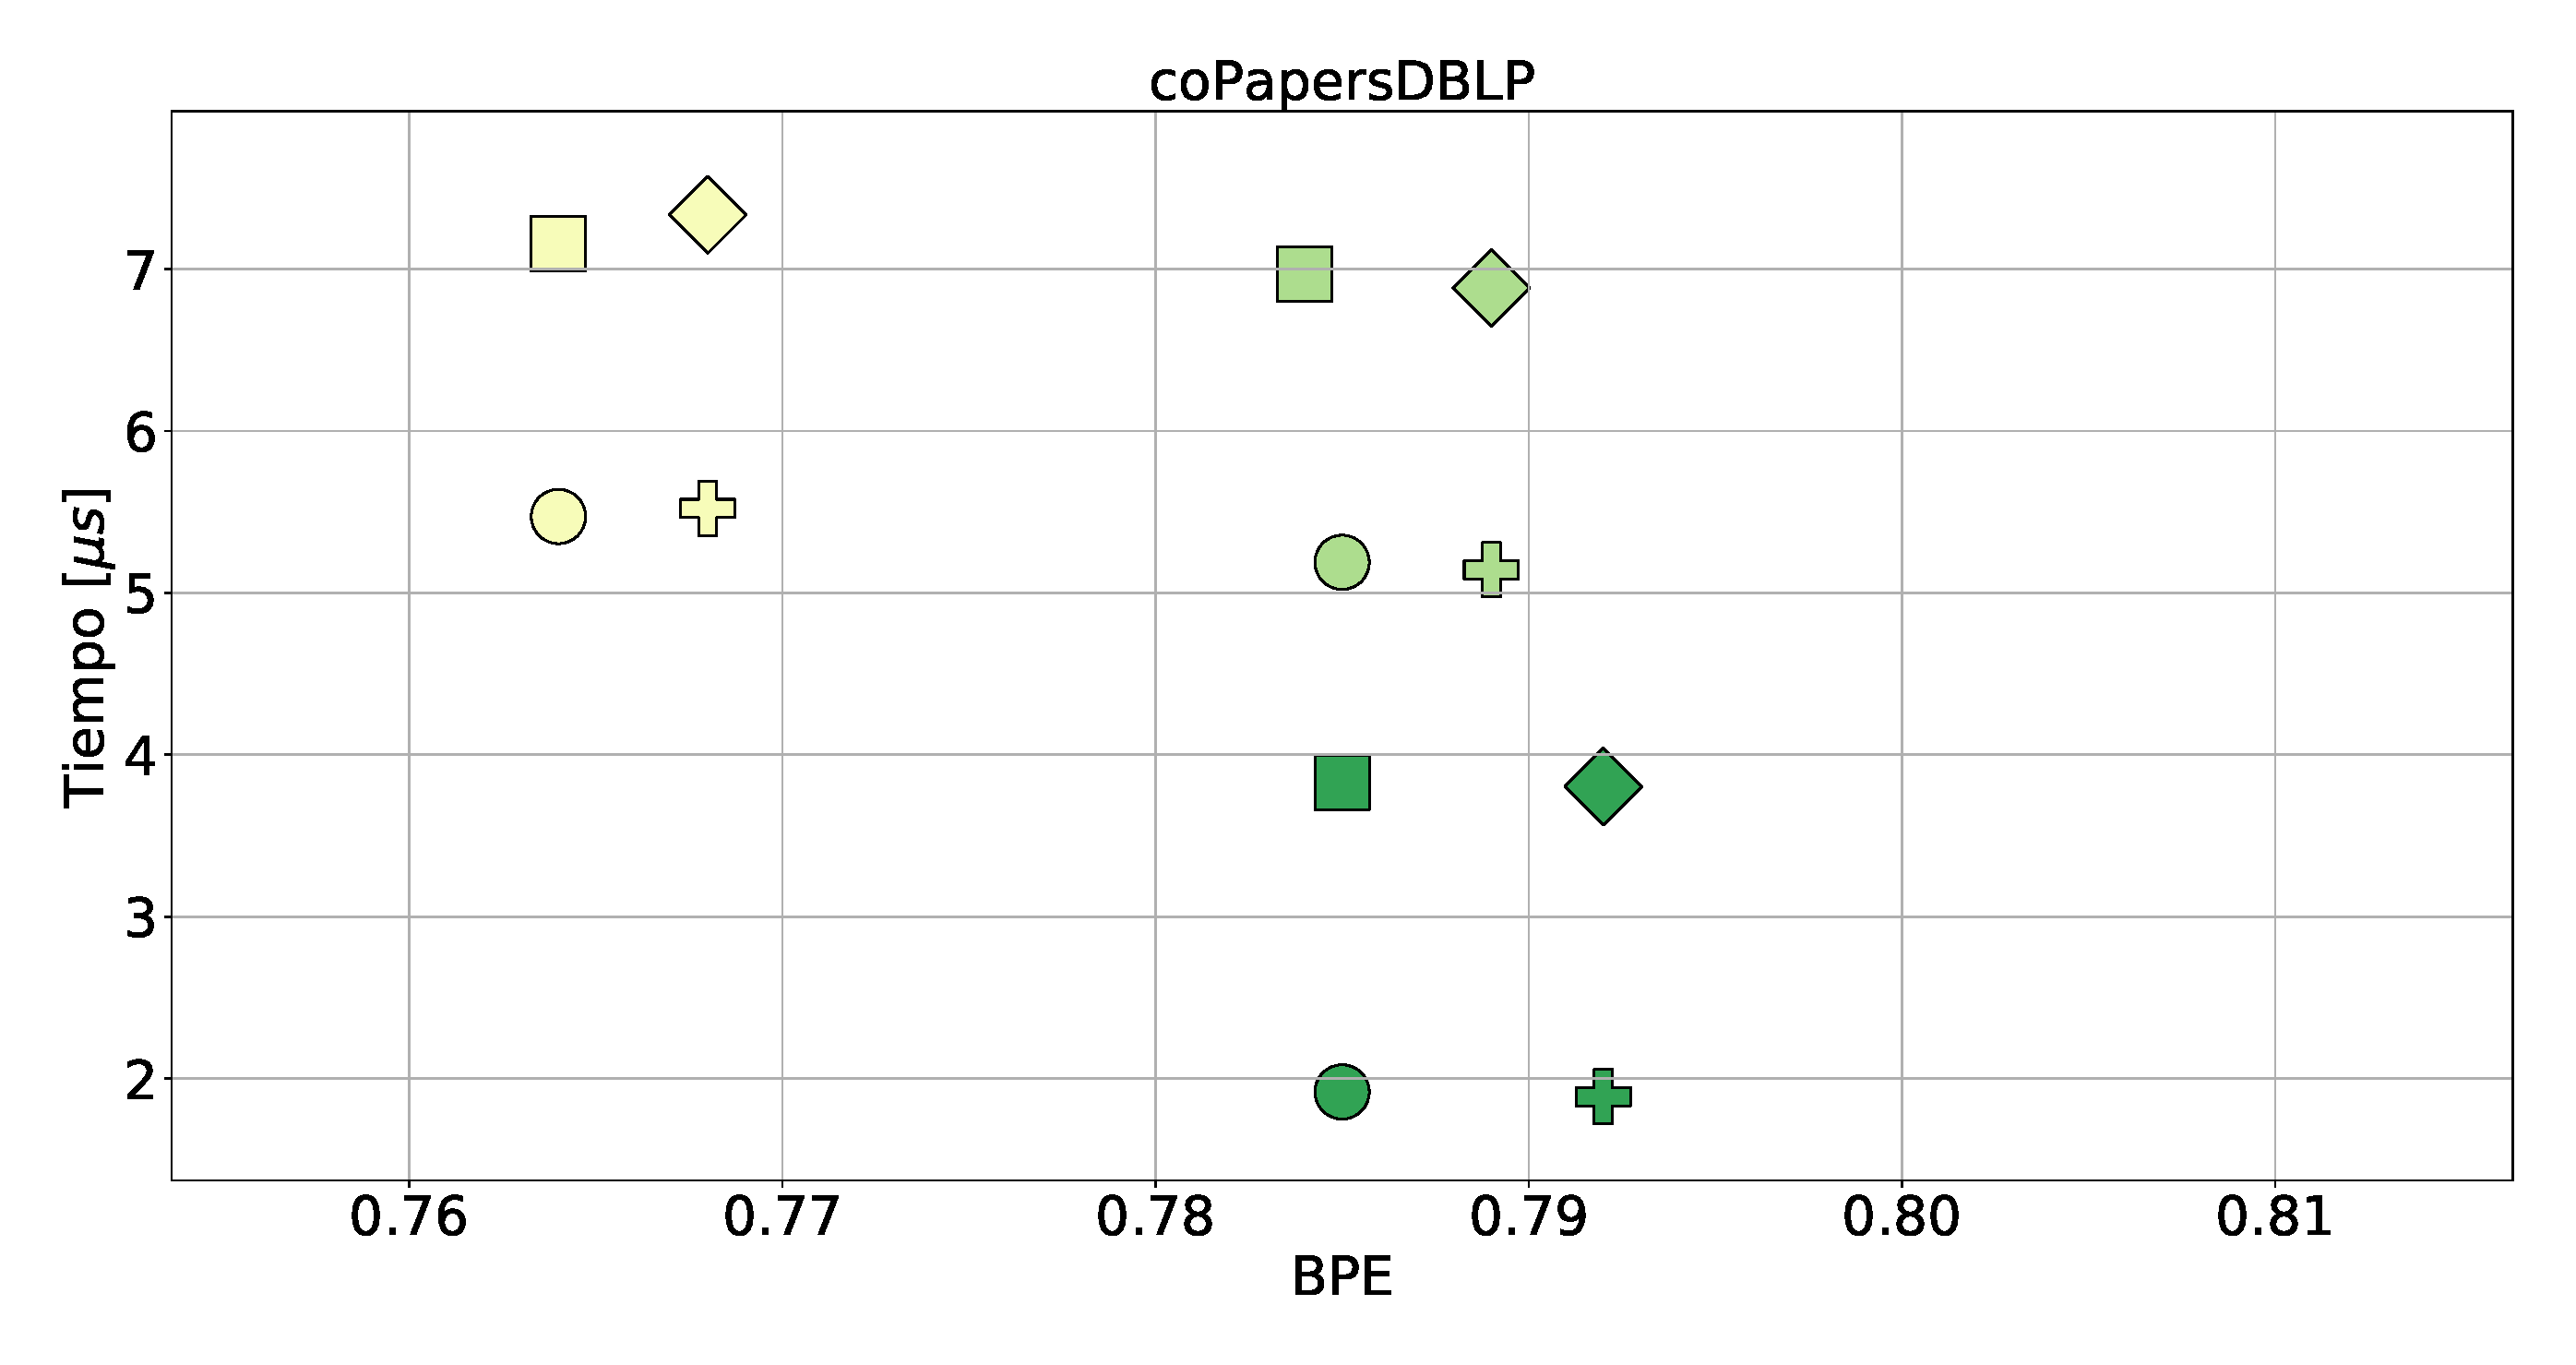
\includegraphics[width=1\linewidth]{img/sdsl/aleatorioBig/coPapersDBLP.pdf}
    			\end{minipage}
    			\begin{minipage}{0.15\textwidth}
    				\centering
    				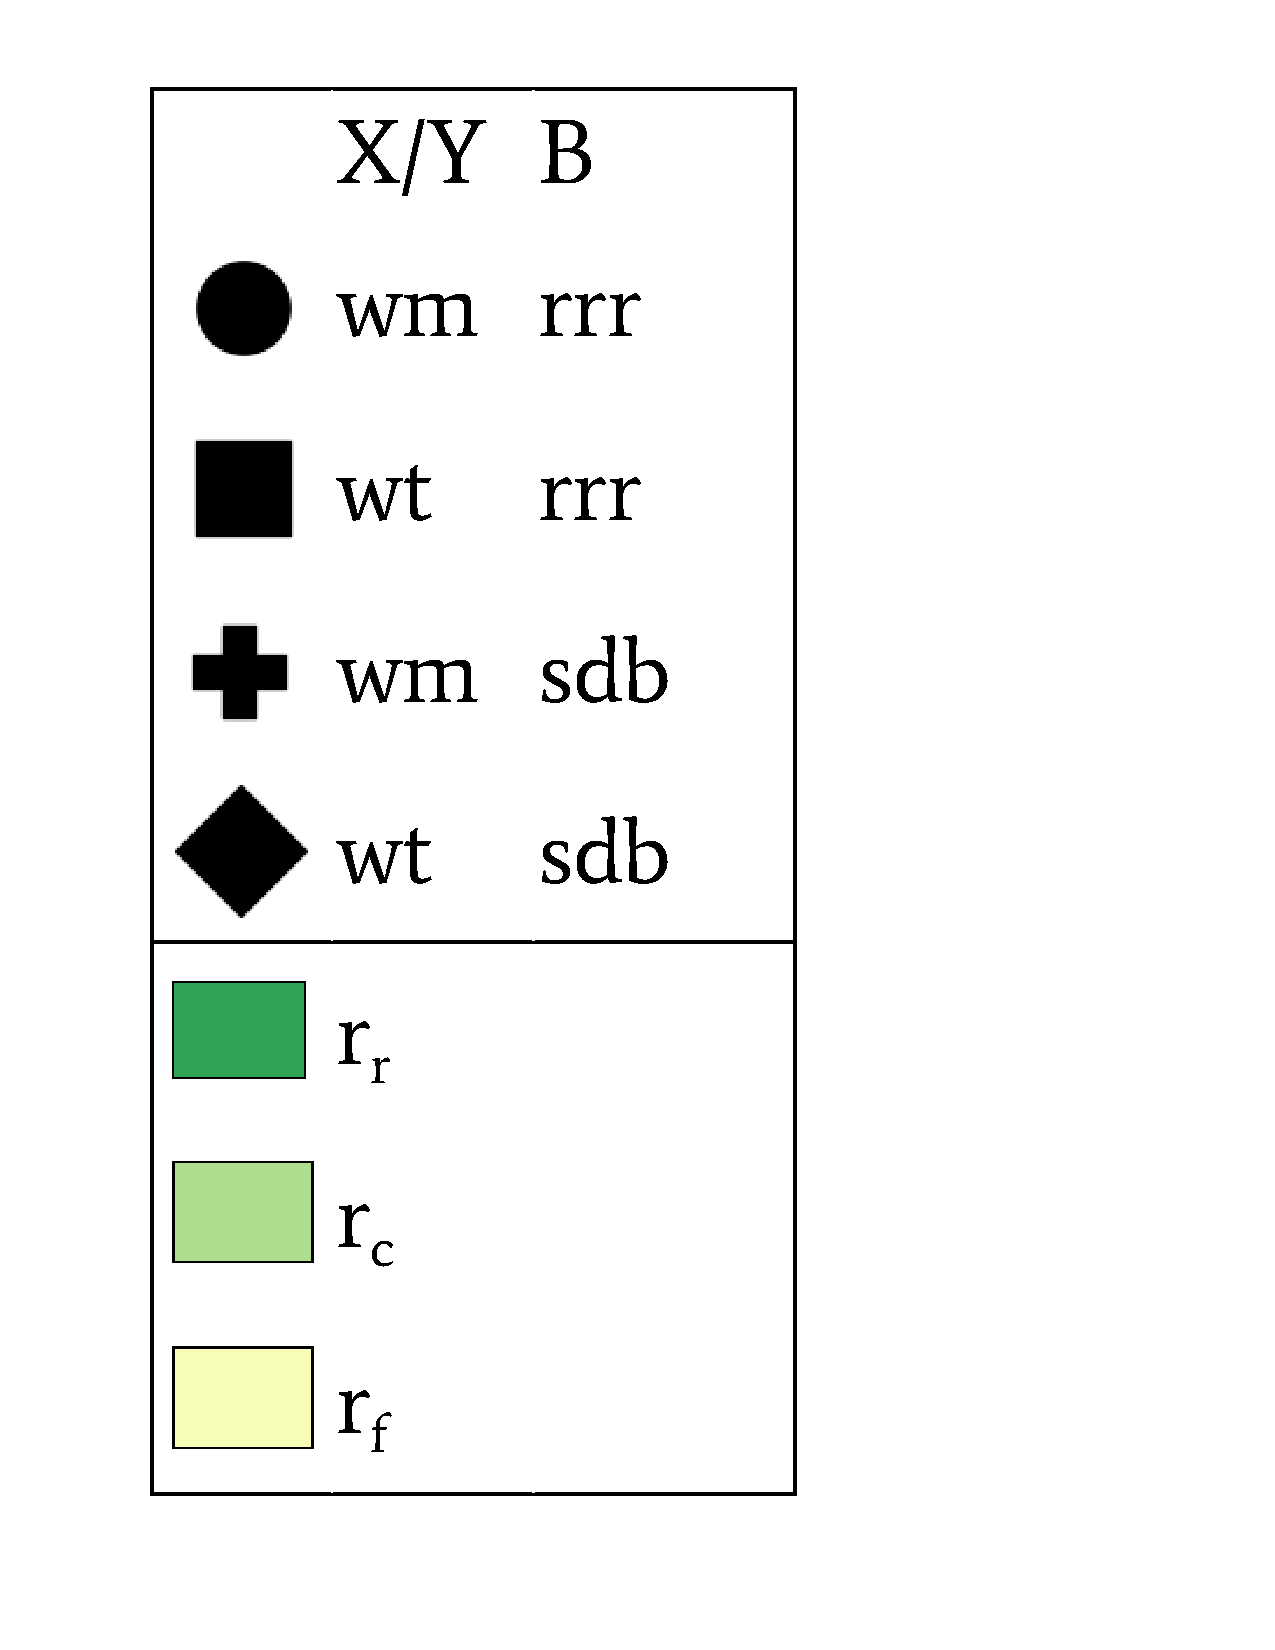
\includegraphics[scale=.22, clip, trim=70 0 0 0]{img/sdsl/label.pdf}
    			\end{minipage}
    			
    			(a)		
    	\end{minipage}
    	
       	\begin{minipage}{1\textwidth}
    			\centering
    			\begin{minipage}{0.8\textwidth}
    				\centering
    				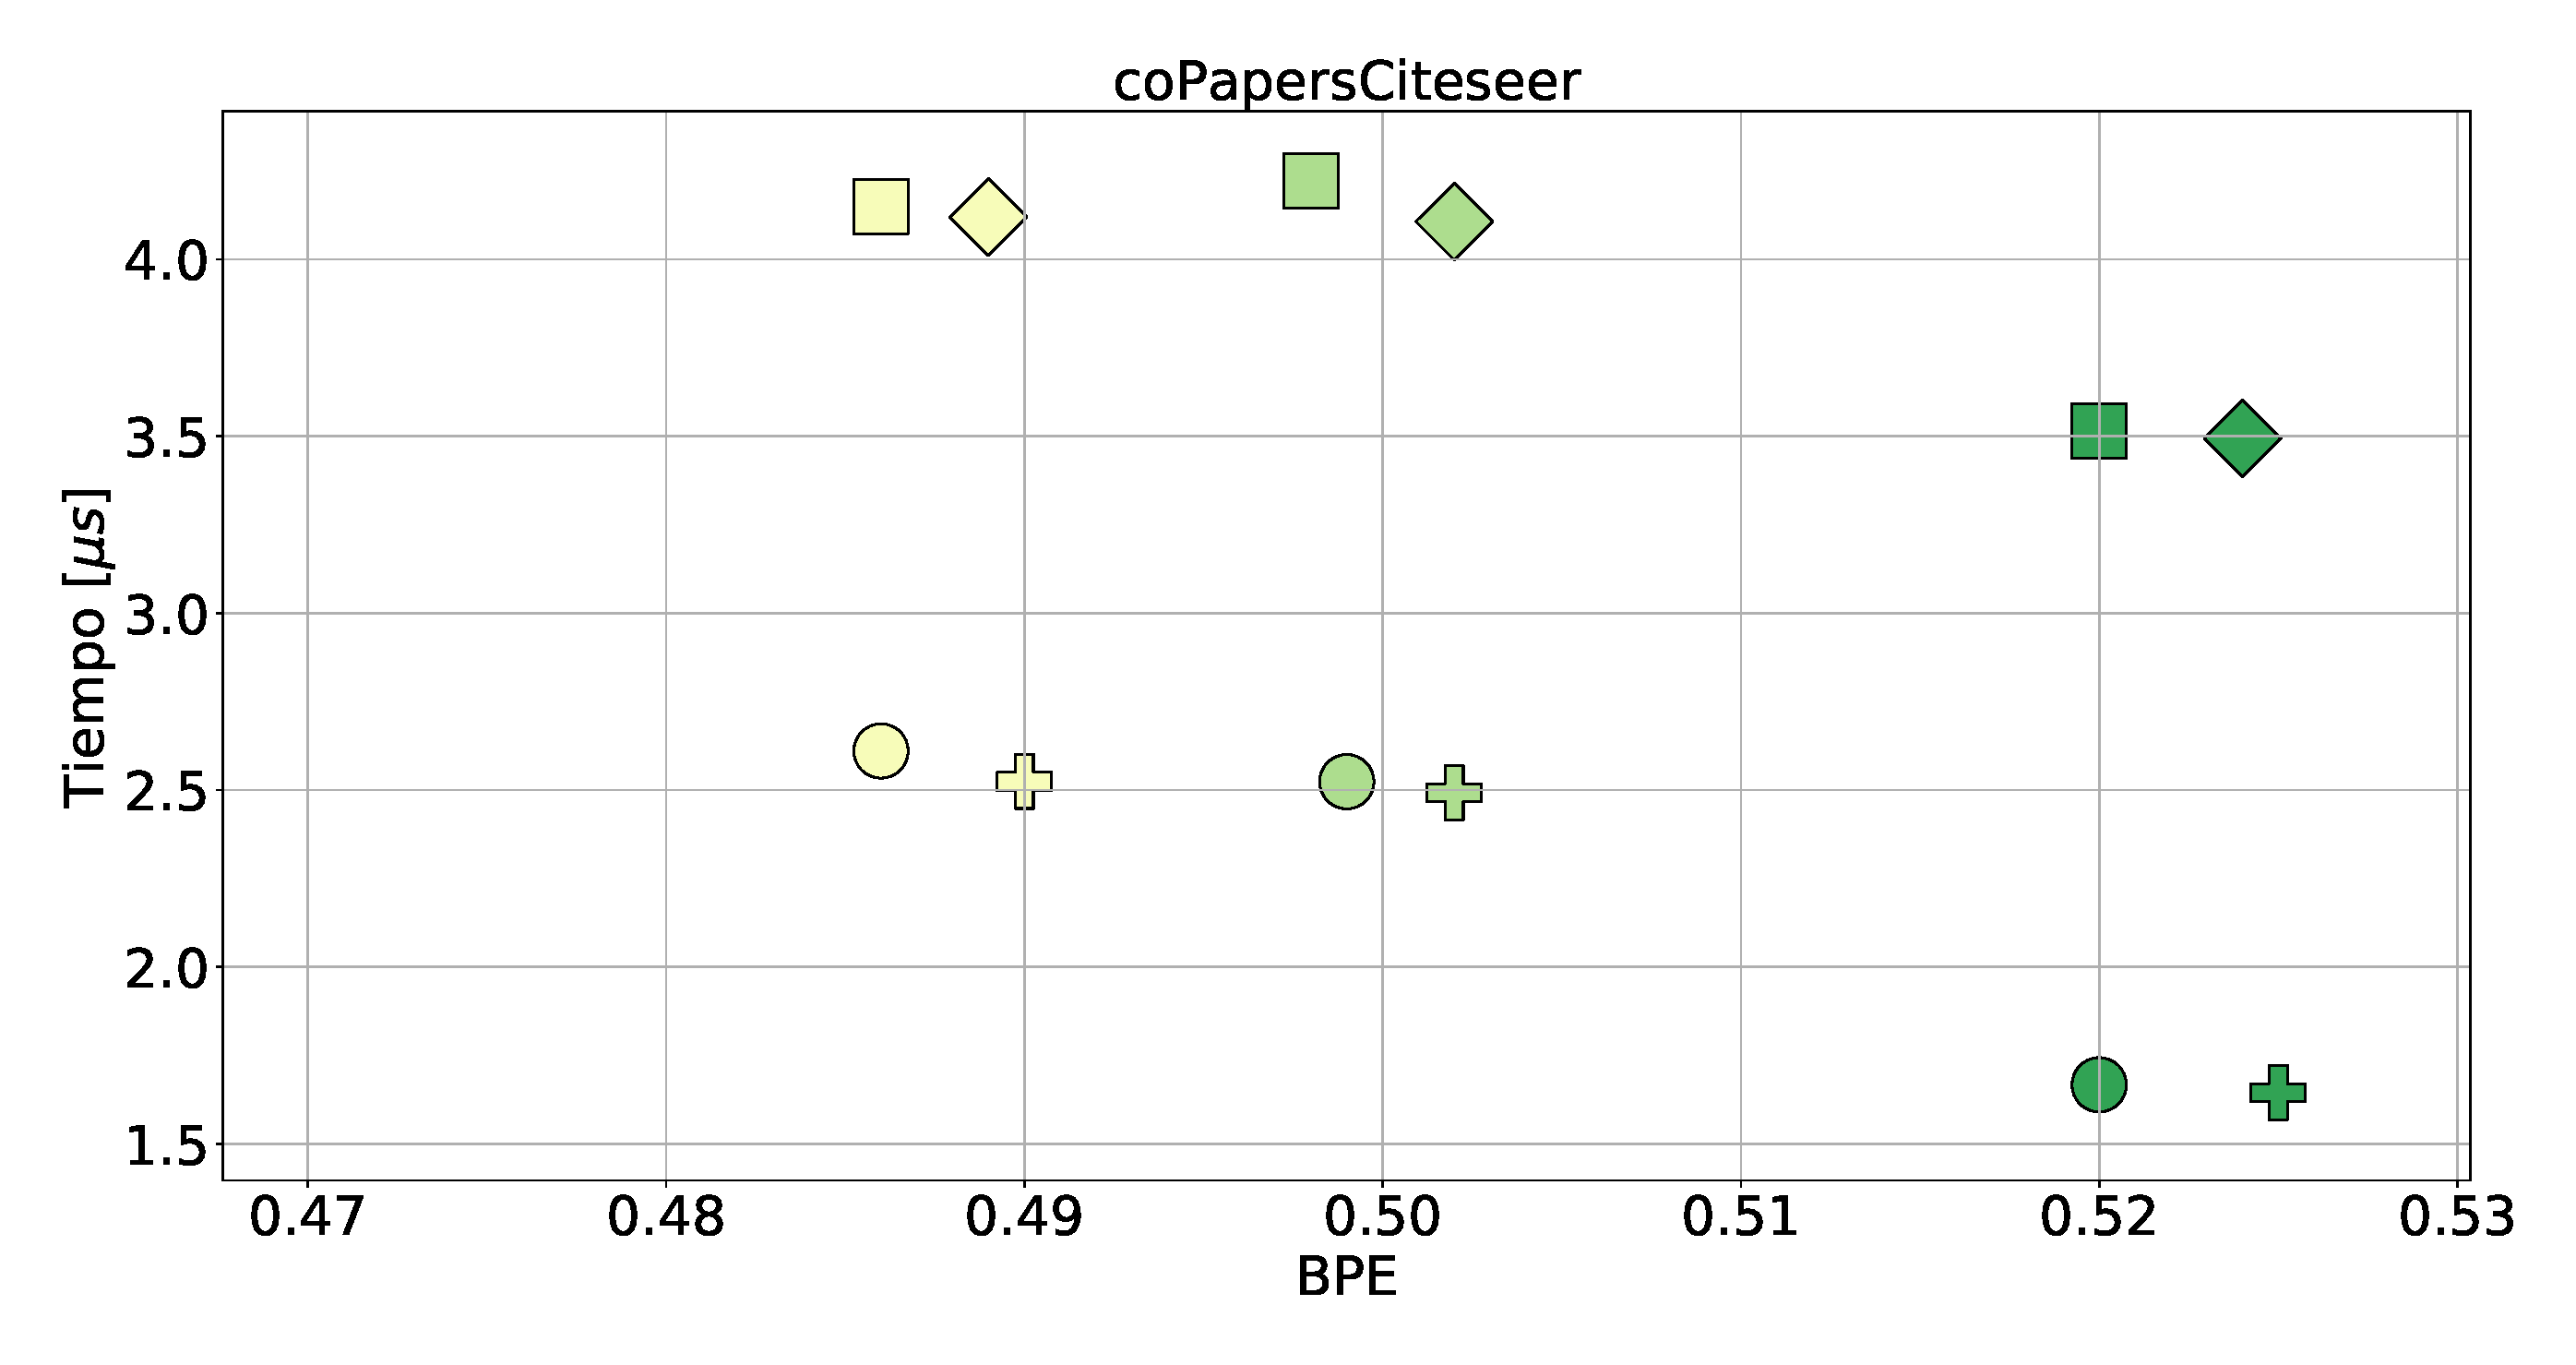
\includegraphics[width=1\linewidth]{img/sdsl/aleatorioBig/coPapersCiteseer.pdf}
    			\end{minipage}
    			\begin{minipage}{0.15\textwidth}
    				\centering
    				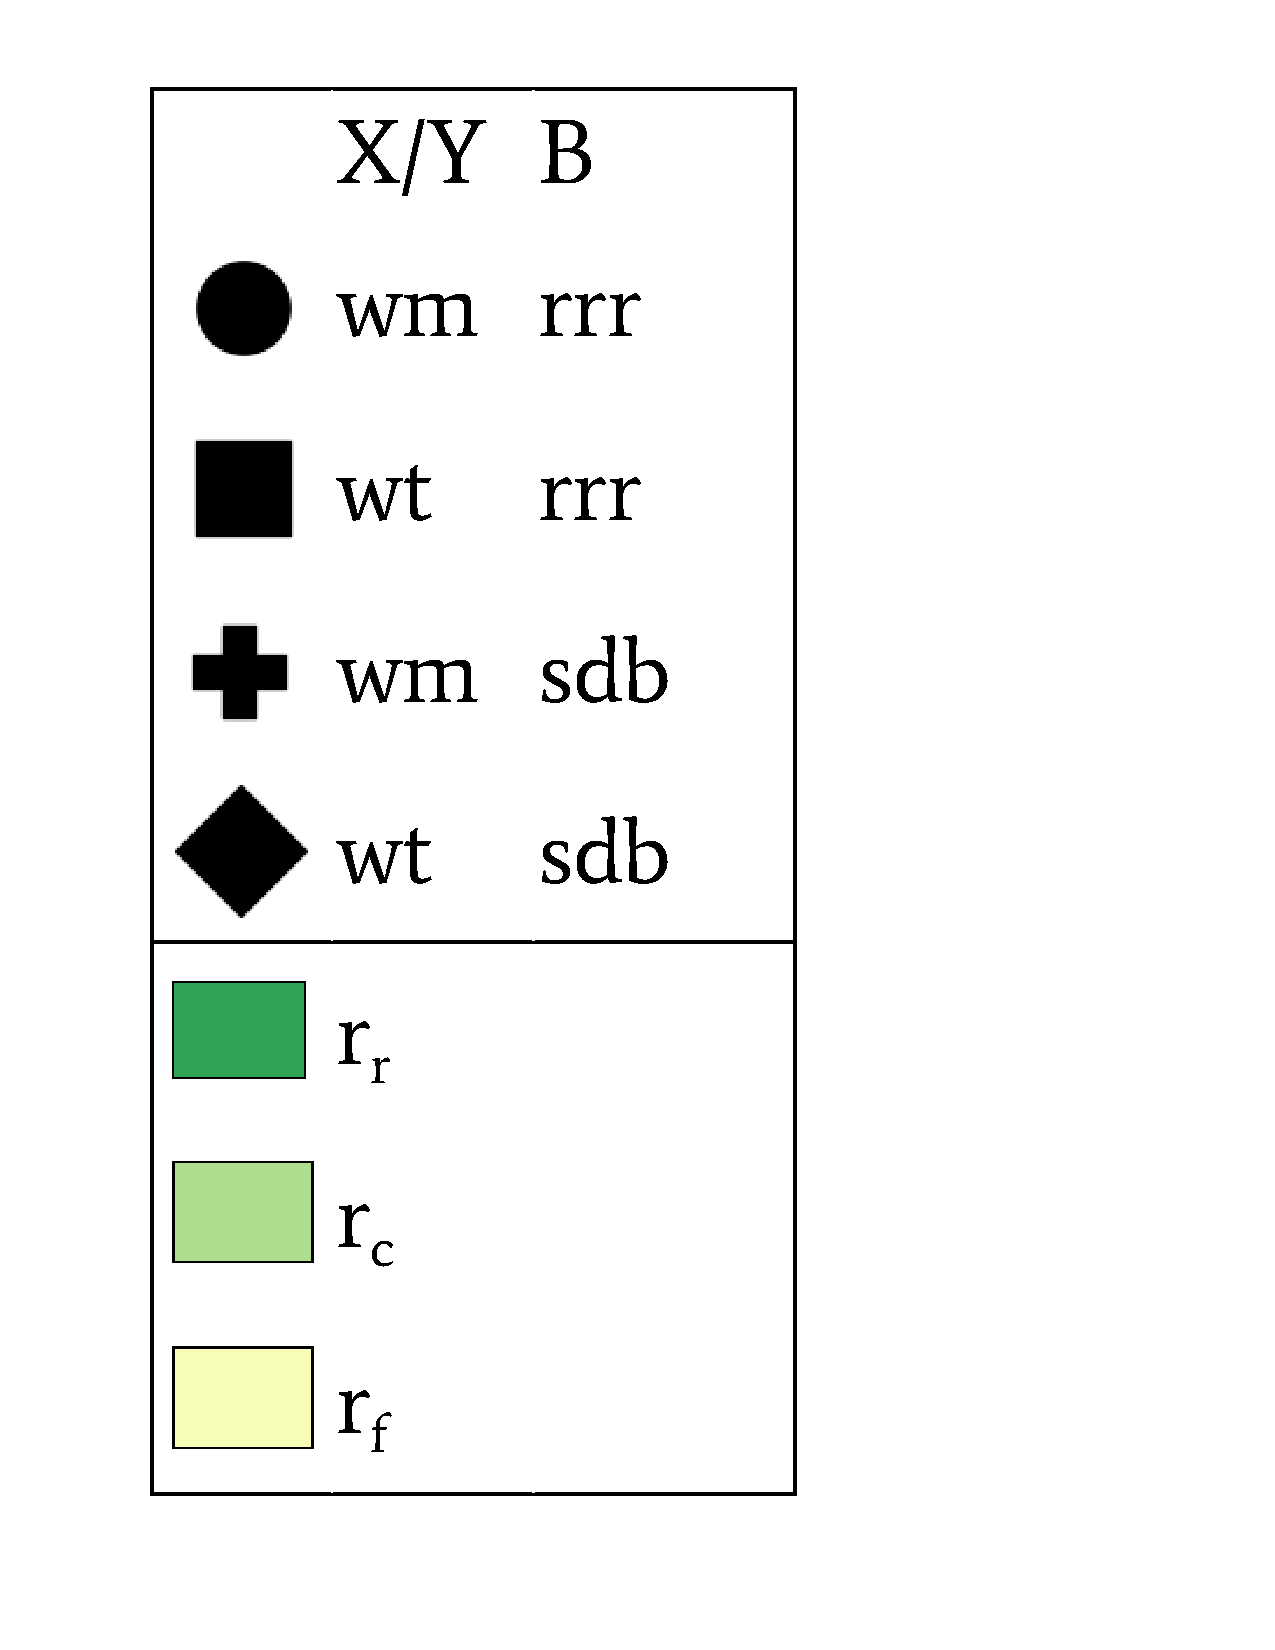
\includegraphics[scale=.22, clip, trim=70 0 0 0]{img/sdsl/label.pdf}
    			\end{minipage}
    			
    			(b)		
    	\end{minipage}
    	
    \caption{BPE y Tiempo de acceso aleatorio medio para posibles estructuras compactas, por cada función de ranking, para los grafos coPapersDBLP y coPapersCiteseer.}
    \label{fig:sdslBPEAle5}
\end{figure}

\begin{figure}
    	\centering
    	\begin{minipage}{1\textwidth}
    			\centering
    			\begin{minipage}{0.8\textwidth}
    				\centering
    				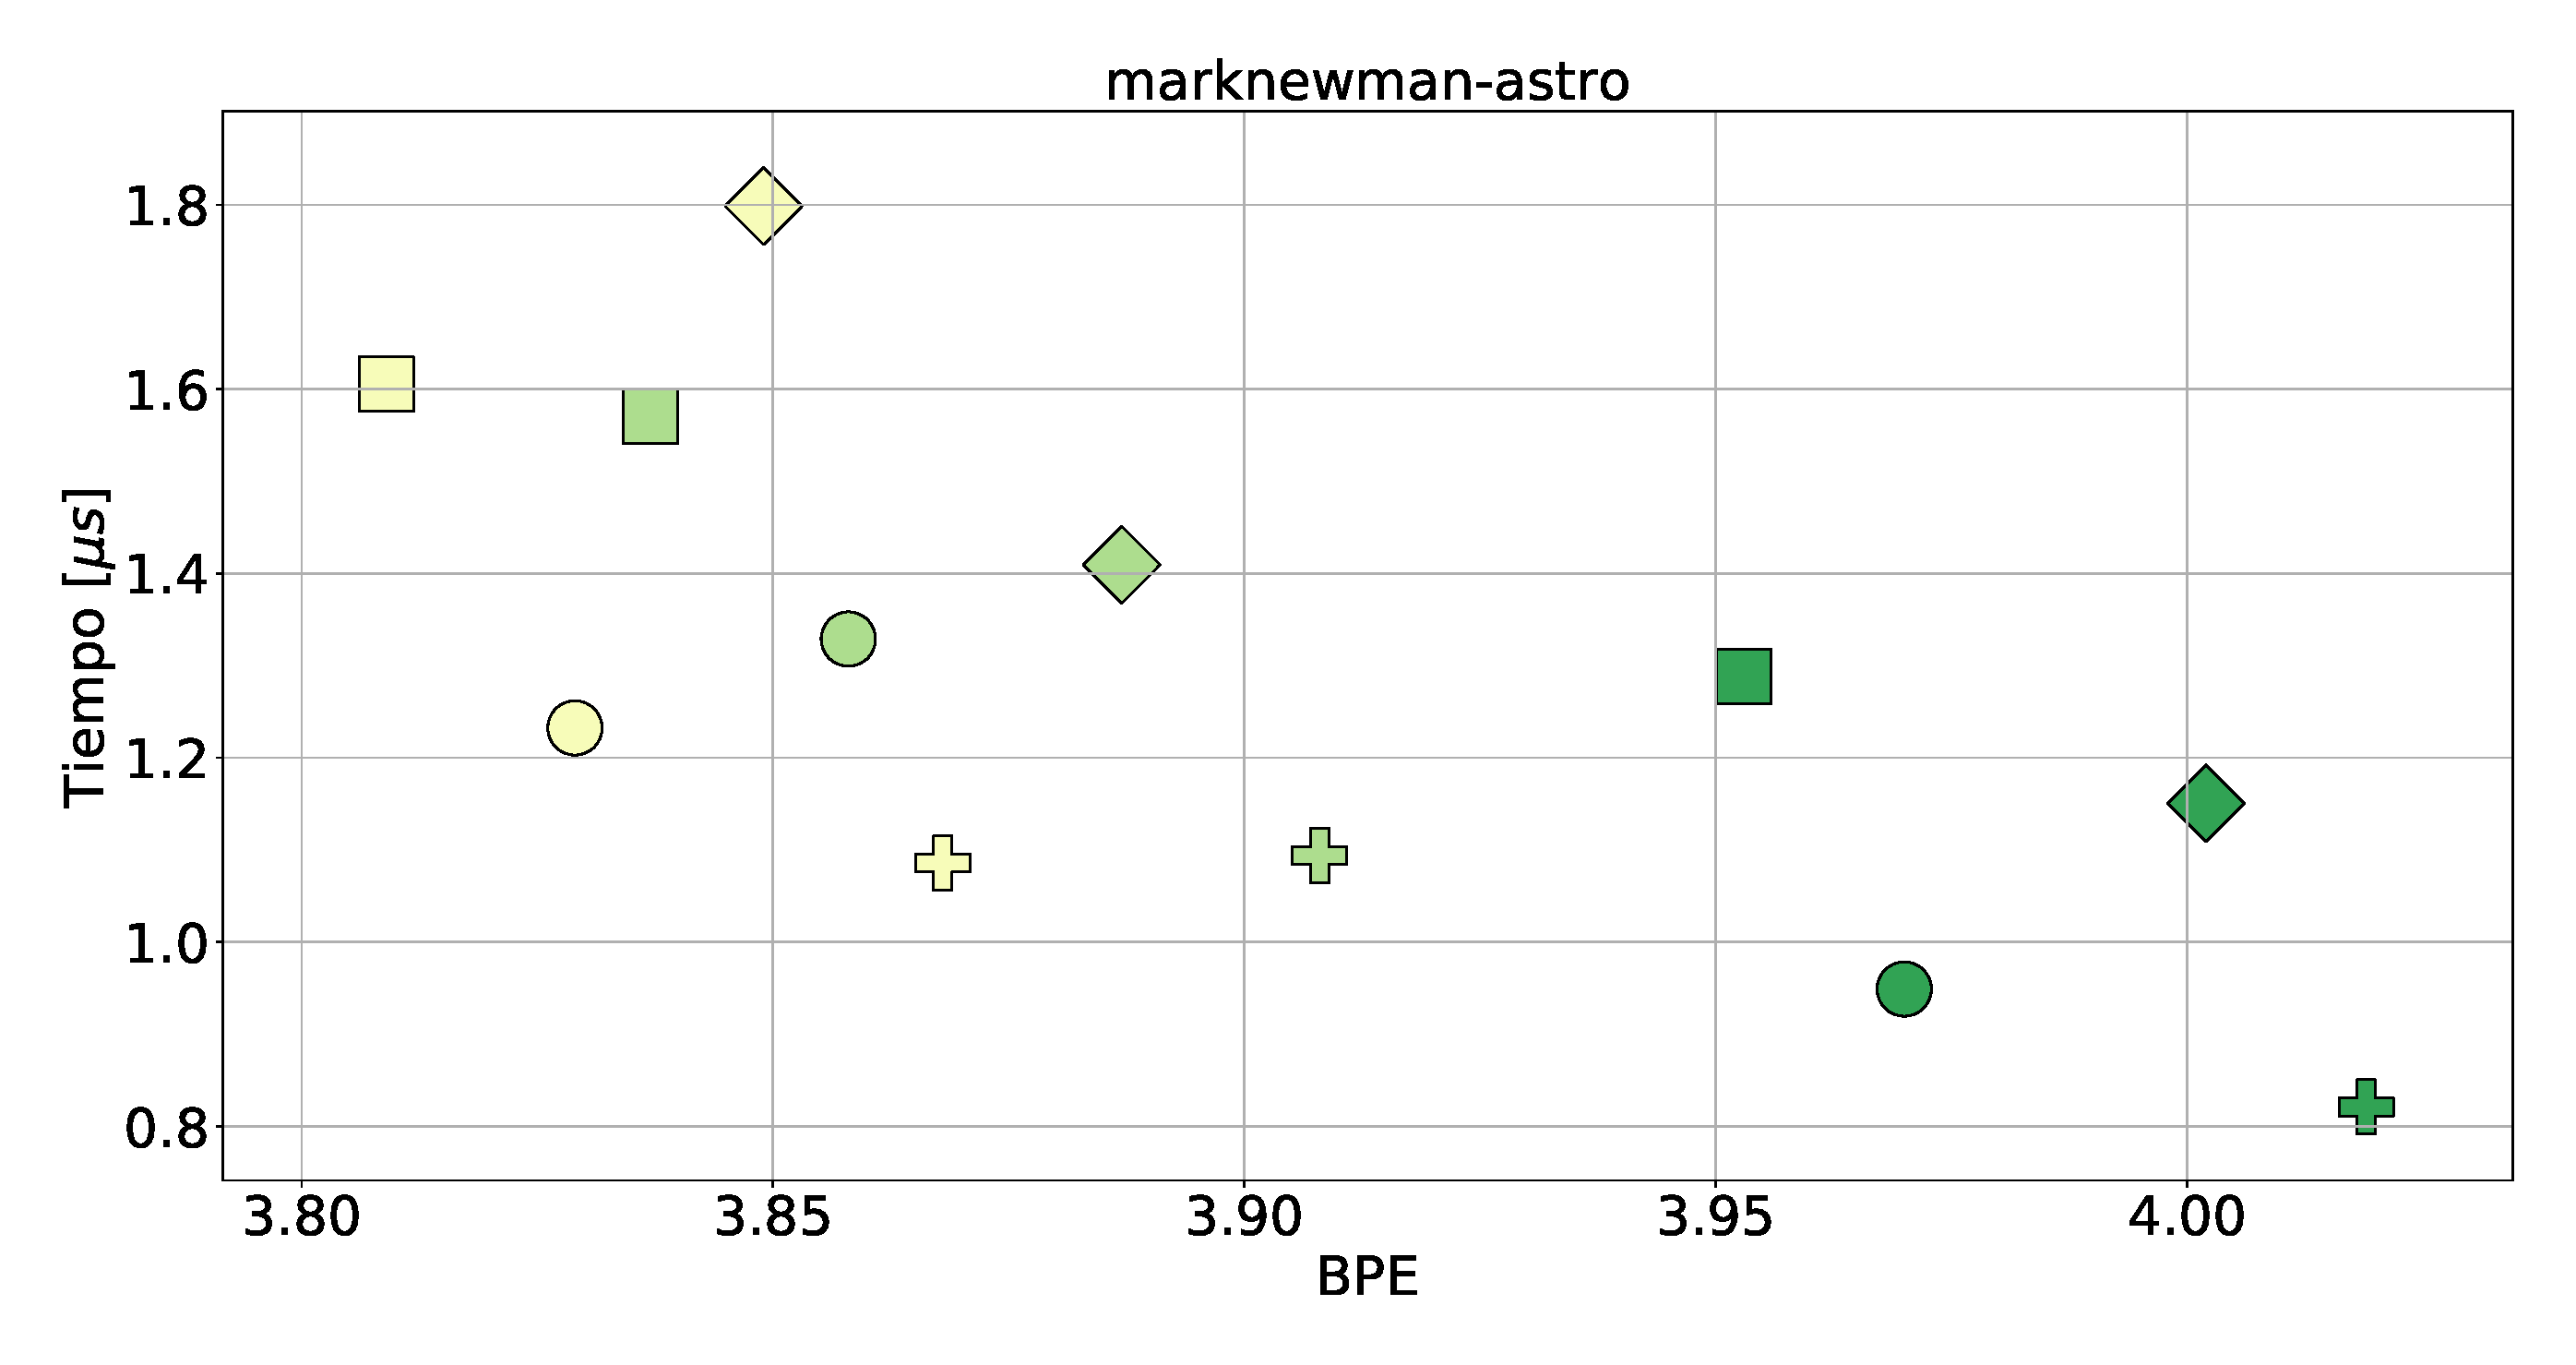
\includegraphics[width=1\linewidth]{img/sdsl/secuencialBig/marknewman-astro.pdf}
    			\end{minipage}
    			\begin{minipage}{0.15\textwidth}
    				\centering
    				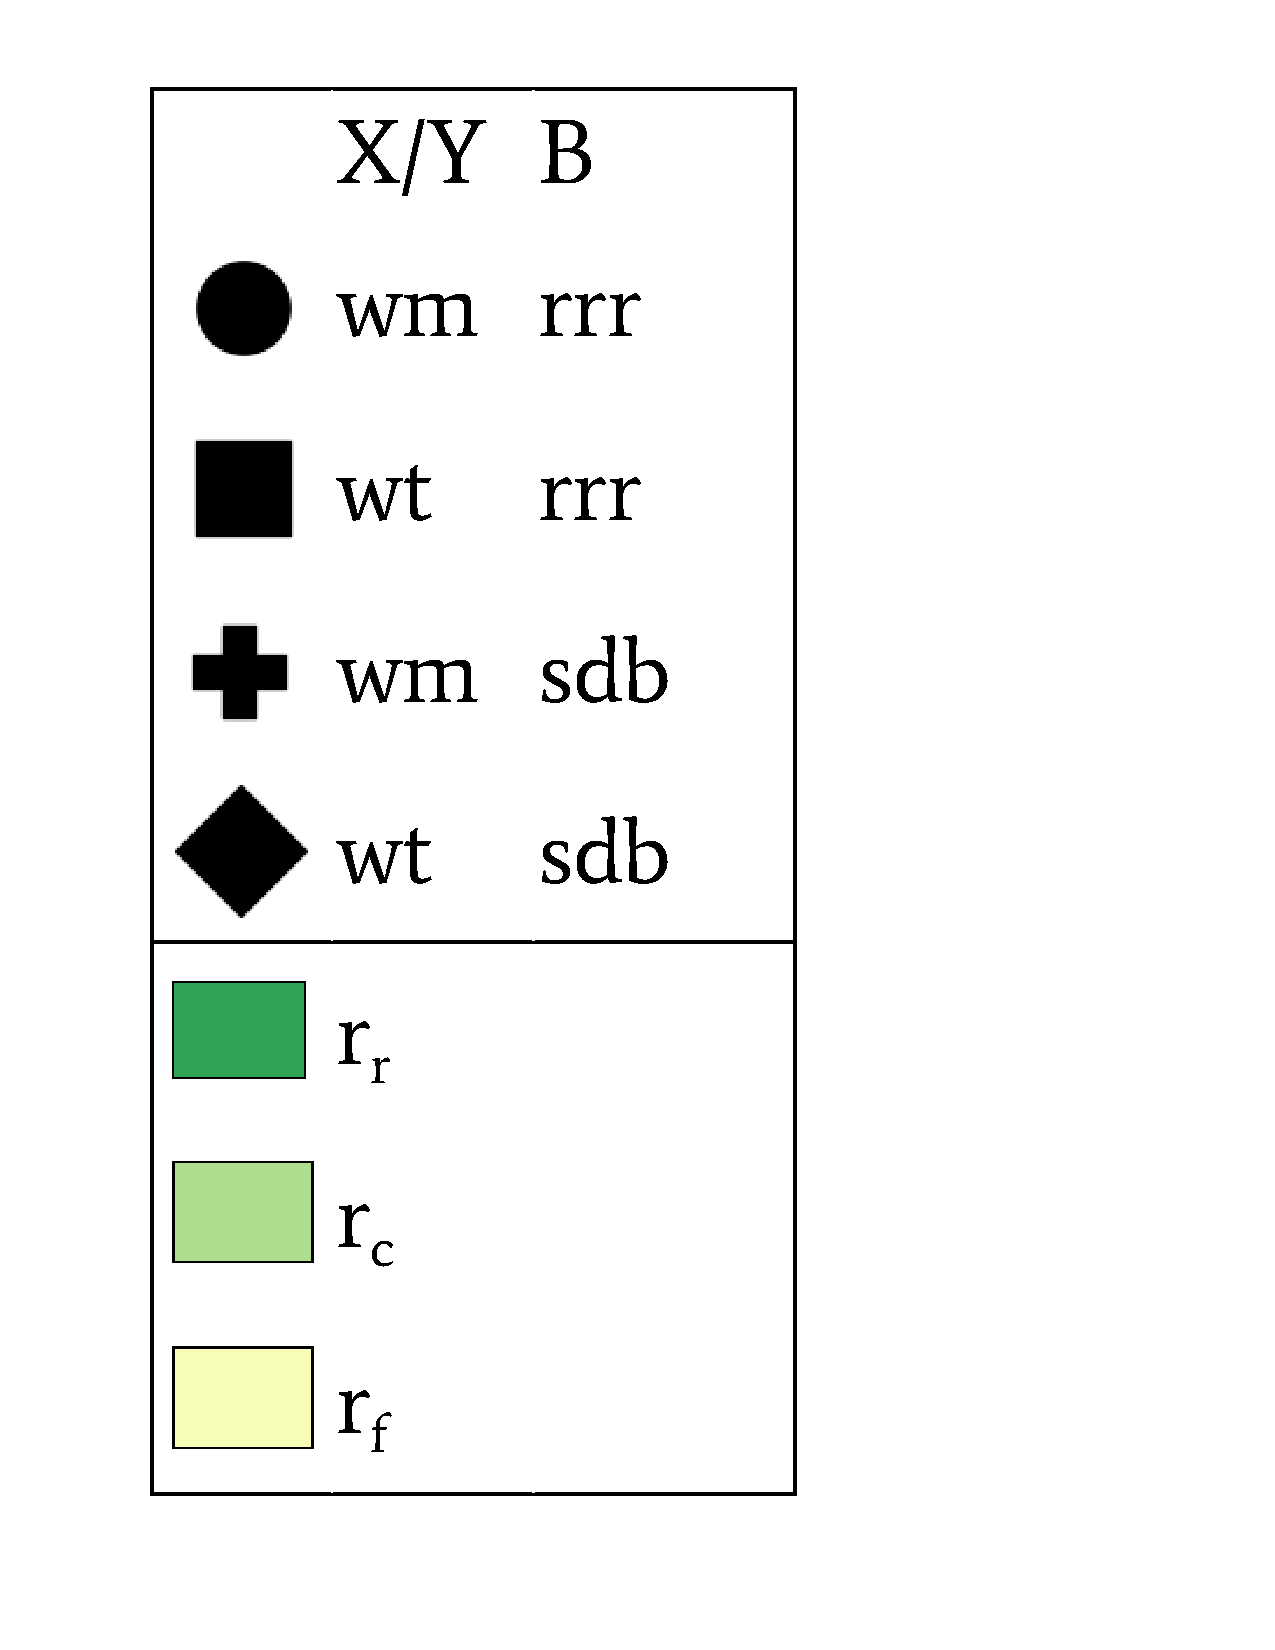
\includegraphics[scale=.22, clip, trim=70 0 0 0]{img/sdsl/label.pdf}
    			\end{minipage}
    			
    			(a)		
    	\end{minipage}
    	
       	\begin{minipage}{1\textwidth}
    			\centering
    			\begin{minipage}{0.8\textwidth}
    				\centering
    				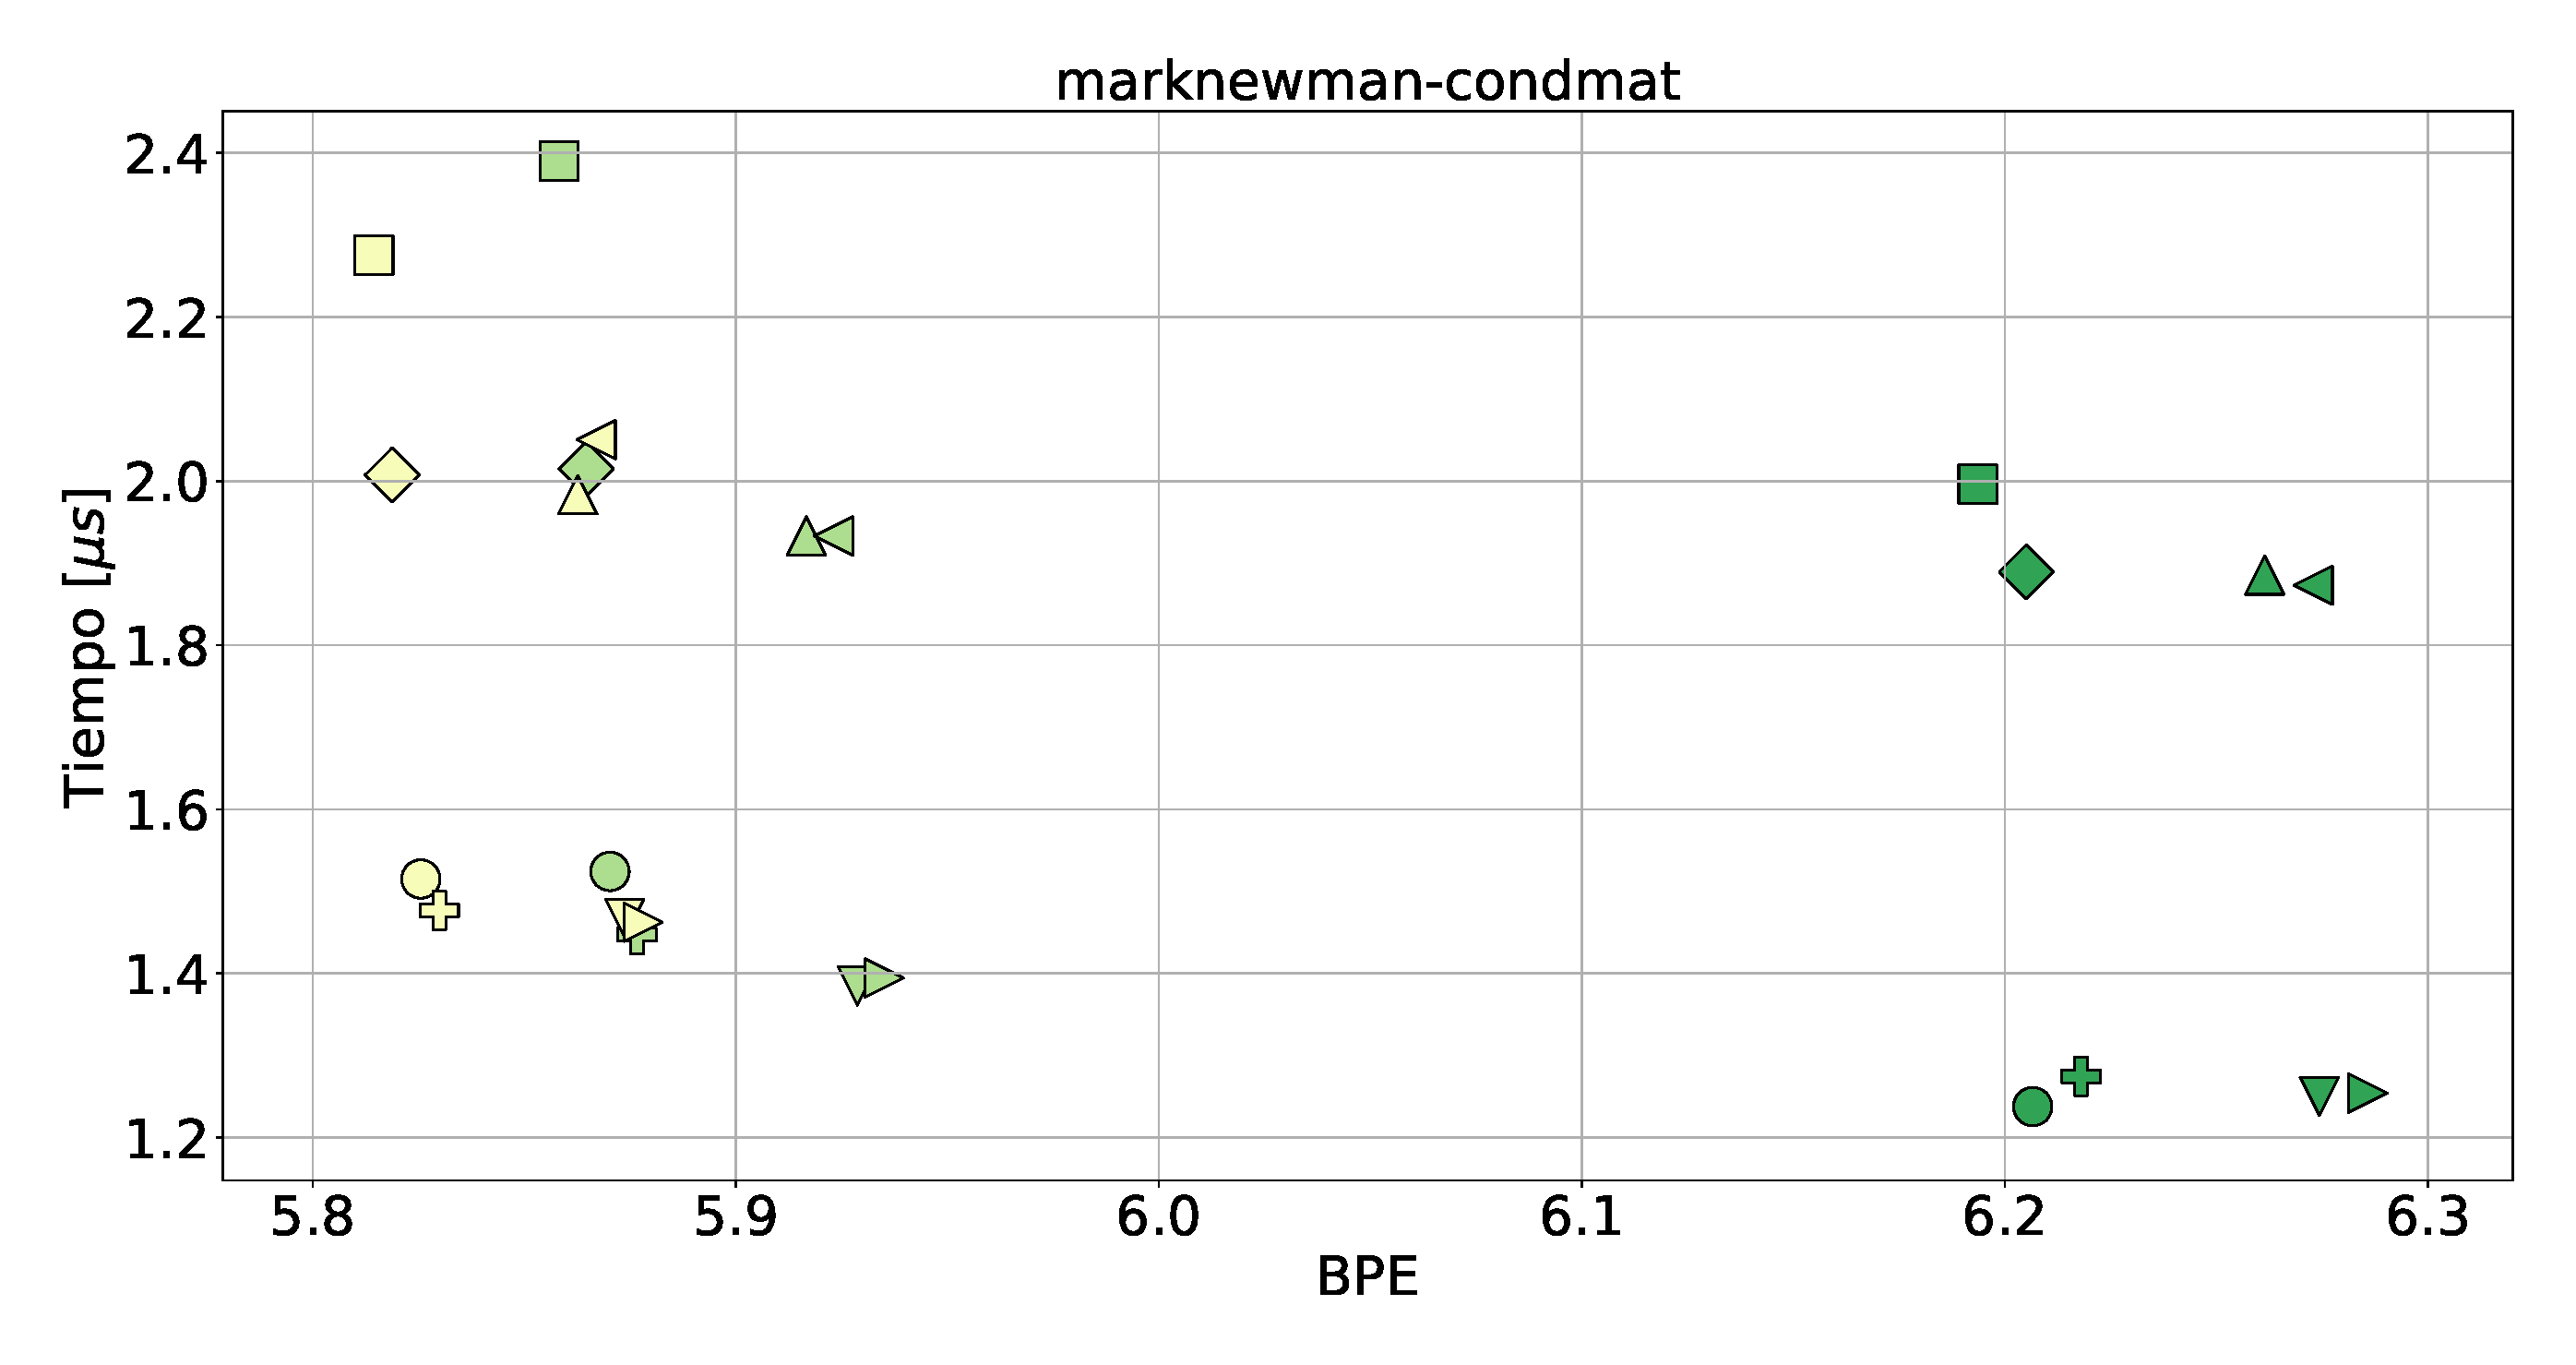
\includegraphics[width=1\linewidth]{img/sdsl/secuencialBig/marknewman-condmat.pdf}
    			\end{minipage}
    			\begin{minipage}{0.15\textwidth}
    				\centering
    				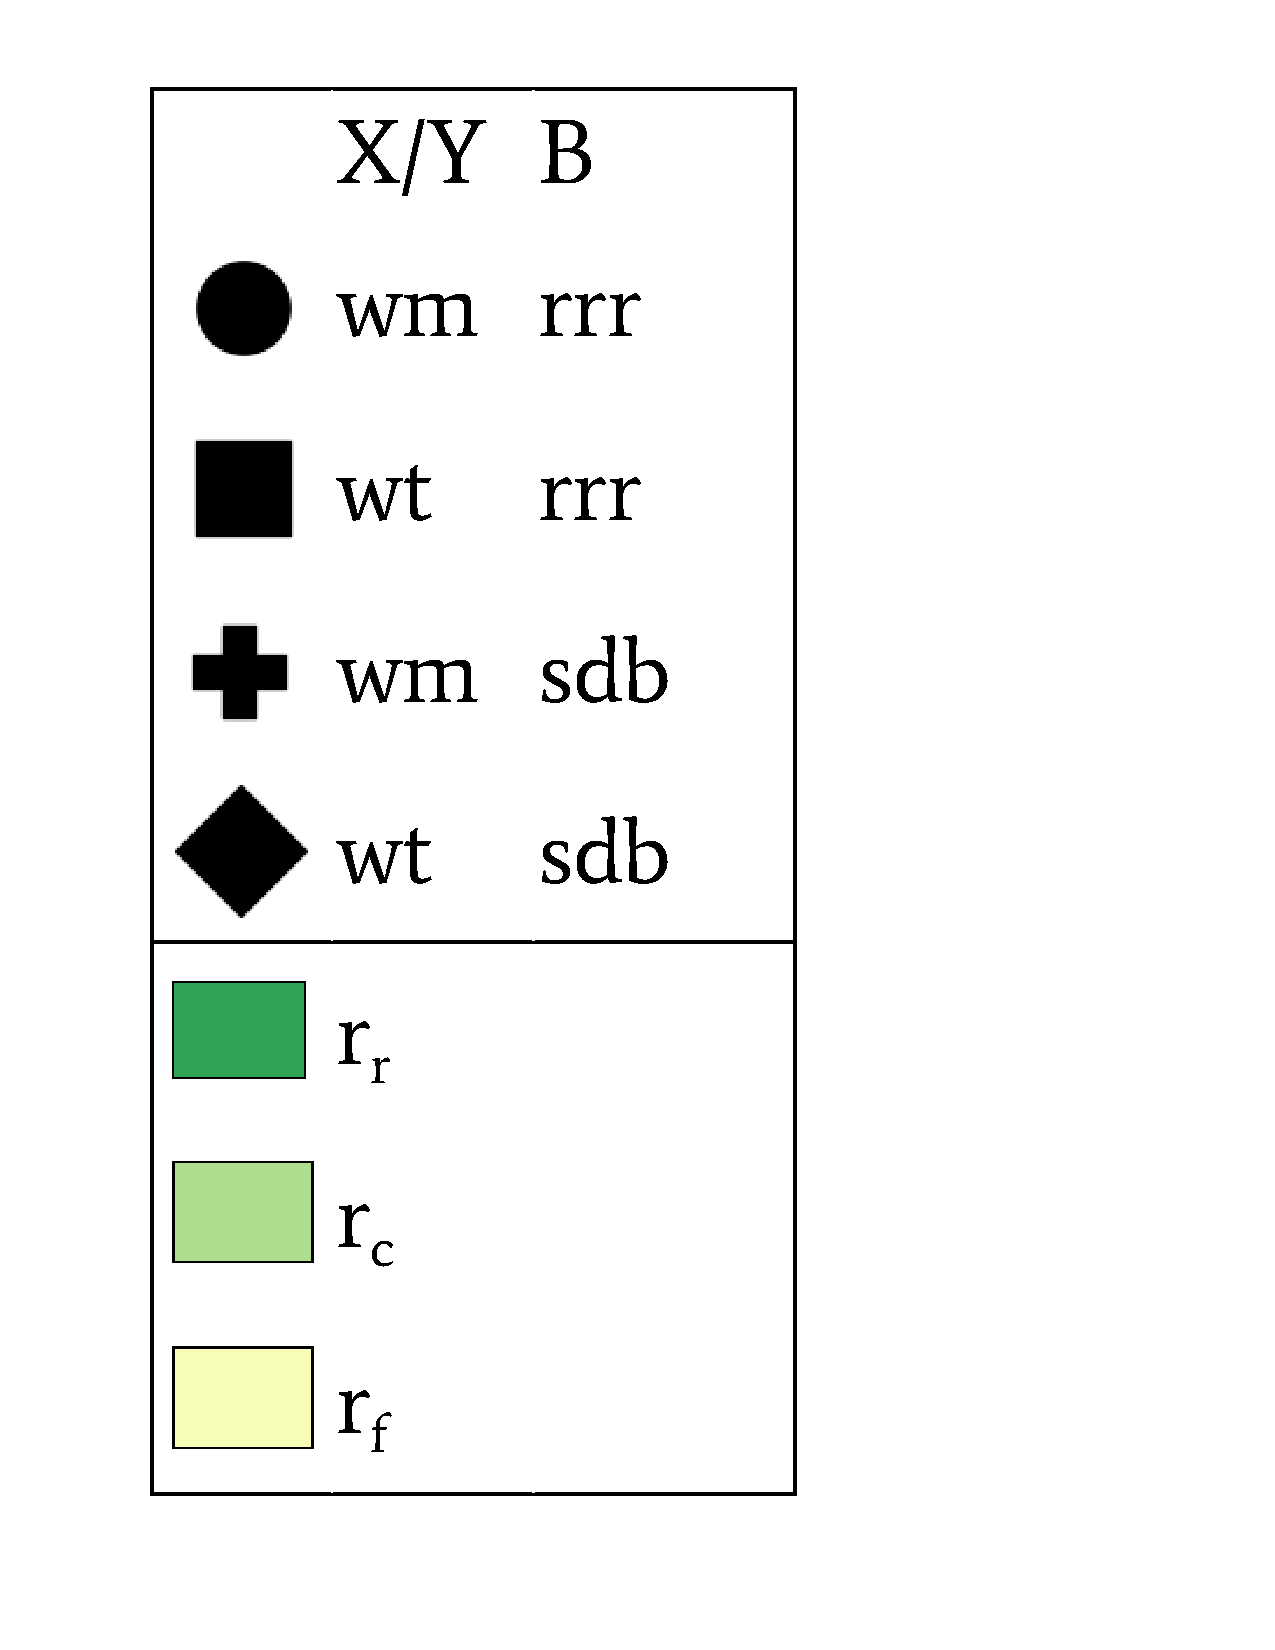
\includegraphics[scale=.22, clip, trim=70 0 0 0]{img/sdsl/label.pdf}
    			\end{minipage}
    			
    			(b)		
    	\end{minipage}
    	
    \caption{BPE y Tiempo de acceso aleatorio medio para posibles estructuras compactas, por cada función de ranking, para los grafos marknewman-astro y marknewman-condmat.}
    \label{fig:sdslBPE2}
\end{figure}

\begin{figure}
    	\centering
    	\begin{minipage}{1\textwidth}
    			\centering
    			\begin{minipage}{0.8\textwidth}
    				\centering
    				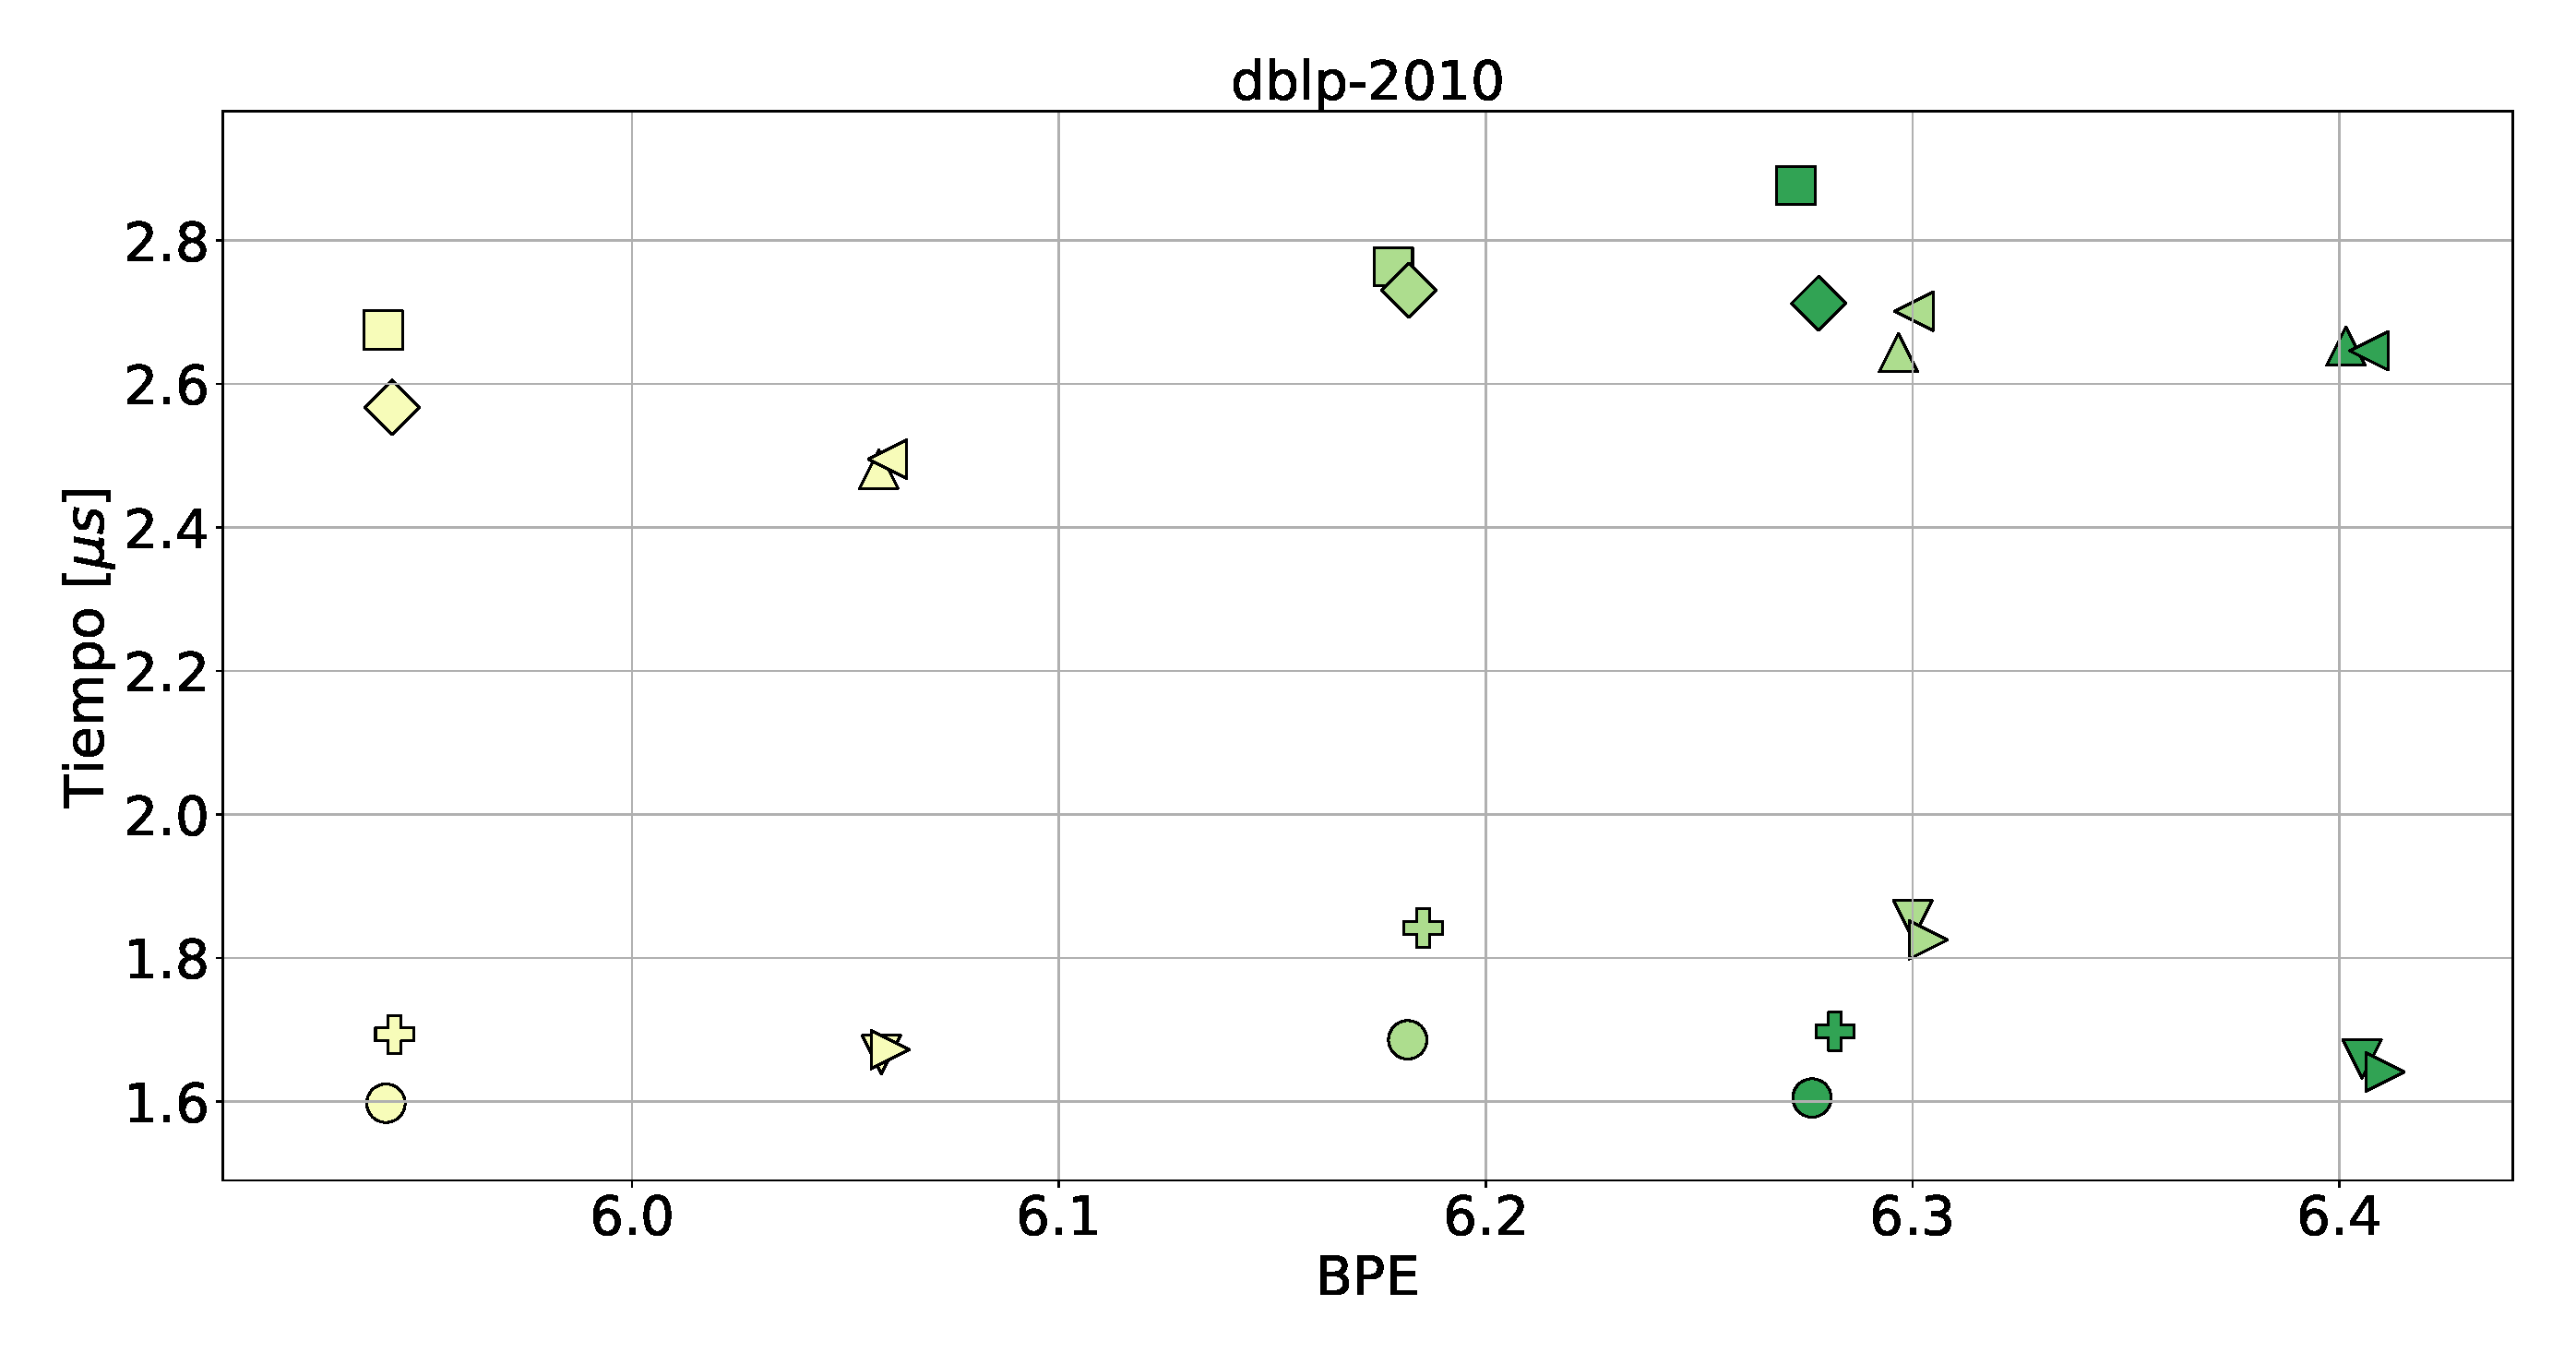
\includegraphics[width=1\linewidth]{img/sdsl/secuencialBig/dblp-2010.pdf}
    			\end{minipage}
    			\begin{minipage}{0.15\textwidth}
    				\centering
    				\includegraphics[scale=.235, clip, trim=70 0 0 0]{img/sdsl/label.pdf}
    			\end{minipage}
    			
    			(a)		
    	\end{minipage}
    	
       	\begin{minipage}{1\textwidth}
    			\centering
    			\begin{minipage}{0.8\textwidth}
    				\centering
    				\includegraphics[width=1\linewidth]{img/sdsl/secuencialBig/dblp-2011.pdf}
    			\end{minipage}
    			\begin{minipage}{0.15\textwidth}
    				\centering
    				\includegraphics[scale=.235, clip, trim=70 0 0 0]{img/sdsl/label.pdf}
    			\end{minipage}
    			
    			(b)		
    	\end{minipage}
    	
    \caption{BPE y Tiempo de acceso secuencial medio para posibles estructuras compactas, por cada función de ranking, para los grafos dblp-2010 y dblp-2011.}
    \label{fig:sdslBPE3}
\end{figure}

\begin{figure}
    	\centering
    	\begin{minipage}{1\textwidth}
    			\centering
    			\begin{minipage}{0.8\textwidth}
    				\centering
    				\includegraphics[width=1\linewidth]{img/sdsl/secuencialBig/snap-dblp.pdf}
    			\end{minipage}
    			\begin{minipage}{0.15\textwidth}
    				\centering
    				\includegraphics[scale=.235, clip, trim=70 0 0 0]{img/sdsl/label.pdf}
    			\end{minipage}
    			
    			(a)		
    	\end{minipage}
    	
       	\begin{minipage}{1\textwidth}
    			\centering
    			\begin{minipage}{0.8\textwidth}
    				\centering
    				\includegraphics[width=1\linewidth]{img/sdsl/secuencialBig/snap-amazon.pdf}
    			\end{minipage}
    			\begin{minipage}{0.15\textwidth}
    				\centering
    				\includegraphics[scale=.235, clip, trim=70 0 0 0]{img/sdsl/label.pdf}
    			\end{minipage}
    			
    			(b)		
    	\end{minipage}
    	
    \caption{BPE y Tiempo de acceso secuencial medio para posibles estructuras compactas, por cada función de ranking, para los grafos snap-dblp y snap-amazon.}
    \label{fig:sdslBPE4}
\end{figure}

\begin{figure}
    	\centering
    	\begin{minipage}{1\textwidth}
    			\centering
    			\begin{minipage}{0.8\textwidth}
    				\centering
    				\includegraphics[width=1\linewidth]{img/sdsl/secuencialBig/coPapersDBLP.pdf}
    			\end{minipage}
    			\begin{minipage}{0.15\textwidth}
    				\centering
    				\includegraphics[scale=.22, clip, trim=70 0 0 0]{img/sdsl/label.pdf}
    			\end{minipage}
    			
    			(a)		
    	\end{minipage}
    	
       	\begin{minipage}{1\textwidth}
    			\centering
    			\begin{minipage}{0.8\textwidth}
    				\centering
    				\includegraphics[width=1\linewidth]{img/sdsl/secuencialBig/coPapersCiteseer.pdf}
    			\end{minipage}
    			\begin{minipage}{0.15\textwidth}
    				\centering
    				\includegraphics[scale=.22, clip, trim=70 0 0 0]{img/sdsl/label.pdf}
    			\end{minipage}
    			
    			(b)		
    	\end{minipage}
    	
    \caption{BPE y Tiempo de acceso secuencial medio para posibles estructuras compactas, por cada función de ranking, para los grafos coPapersDBLP y coPapersCiteseer.}
    \label{fig:sdslBPE5}
\end{figure}



\section{Comparación de funciones de ranking}

A continuación se compararán las estructuras compactas resultantes, usando las tres funciones de ranking basadas en la frecuencia del vértice en los cliques maximales $r_{f}(u)$, en la cantidad de vecinos en los cliques del vértice $r_{c}(u)$, y la razón entre ambas funciones $r_{r}(u)$. 

En la Figura~\ref{fig:bpe3} se muestran los BPE de las estructuras compactas finales, aplicando las funciones de ranking en la heurística de clusterización. Se puede apreciar que tanto $r_{f}(u)$ como $r_{c}(u)$ logran un nivel de compresión muy similar con un BPE parecido en todos los casos, y si bien $r_{r}(u)$ obtiene un BPE mayor siempre, tampoco es tan lejano al resultado de las demás funciones. Si este parámetro fuera el único a considerar para elegir la mejor función, $r_{f}(u)$ es siempre la que obtiene el menor BPE, pero es necesario profundizar en la conformación de la estructura.

%\begin{table}
	\caption{BPE de las estructuras compactas obtenidas con las funciones de ranking para los grafos.}
	\rowcolors{2}{white}{gray!10}
	\label{table:bpeRanking}
	\centering
	\begin{tabular}{l|r|r|r}
		\toprule
		Grafo & $BPE_{rf}$ & $BPE_{rc}$ & $BPE_{rr}$ \\
		\midrule
		marknewman-astro & 4,208 & 4,246 & 4,454 \\
		marknewman-condmat & 5,826 & 5,870 & 6,207 \\
		dblp-2010 & 5,942 & 6,182 & 6,276 \\
		dblp-2011 & 6,499 & 6,656 & 6,878 \\
		snap-dblp & 6,602 & 6,702 & 7,199 \\
		snap-amazon & 9,996 & 10,082 & 10,500 \\
		ca-coauthors & 0,744 & 0,770 & 0,802 \\
         \bottomrule
	\end{tabular}
\end{table}
 
\begin{figure}
    	\centering
    	\includegraphics[width=1\linewidth]{img/bpe3.pdf}
    	
    \caption{BPE de las estructuras compactas para las funciones de ranking.}
    \label{fig:bpe3}
\end{figure}


En la Figura~\ref{fig:nPartitions} se presentan la cantidad de particiones que contiene las estructuras compactas para cada función de ranking. Se aprecia con bastante claridad que la función $r_{r}(u)$ genera más particiones que las otras dos, y dado que el BPE expuesto en la Figura~\ref{fig:bpe3} no refleja esta diferencia, se puede intuir que las particiones son más pequeñas. Para profundizar en este punto, se estudiará la composición de las secuencias de las estructuras compactas para cada función de ranking.

\begin{figure}
    	\centering
    	\includegraphics[width=1\linewidth]{img/Npartitions3.pdf}
    	
    \caption{Número de particiones en las estructuras compactas para las funciones de ranking.}
    \label{fig:nPartitions}
\end{figure}


En la Figura~\ref{fig:proportionBits}(a) se ilustra la proporción de bits para cada secuencia dentro de la estructura compacta, para cada función de ranking. En la Figura~\ref{fig:proportionBits}(b) se ilustra la misma proporción normalizada. Como se puede observar, la secuencia que más aporta para todos los casos es la de vértices \textit{X}, seguida casi siempre de la secuencia de bytes \textit{BB}, luego \textit{Y} y finalmente la secuencia de bits \textit{B}. Nuevamente las funciones de ranking $r_{f}(u)$ y $r_{c}(u)$ tienen resultados similares, y para la función $r_{r}(u)$ la secuencia \textit{X} aumenta su proporción mientras que \textit{BB} disminuye. Esto podría afectar positivamente el tiempo de respuesta de los algoritmos propuestos, ya que todos requieren comparar los bytes de \textit{BB} de cada partición entre ellos, y si hay menos bytes requerirá menos tiempo.

\begin{figure}
    	\centering
    	\begin{minipage}{1\textwidth}
    		\centering
    		\includegraphics[width=1\linewidth]{img/bits.pdf}
    		
    		(a)
    	\end{minipage}  
    	\begin{minipage}{1\textwidth}
    		\centering
    		\includegraphics[width=1\linewidth]{img/bitsNorm.pdf}
    		
    		(b)
    	\end{minipage}  
    \caption{(a) Proporción de bits por cada secuencia en la estructura compacta, para cada función de ranking. (b) Proporción normalizada.}
    \label{fig:proportionBits}
\end{figure}


Para estudiar la composición de las particiones para cada función de ranking, en la Figura~\ref{fig:maxNodes} se ilustran la cantidad máxima de vértices en la secuencia \textit{X} por partición, y en la Figura~\ref{fig:maxBytes} la cantidad máxima de bytes por vértice en la secuencia \textit{BB} de las estructuras compactas resultantes. Como se puede apreciar, la función $r_{r}(u)$ presenta consistentemente los menores valores entre las tres funciones, lo que permite asegurar que es la que mejor agrupa y usa el espacio de las particiones en la estructura compacta.

\begin{figure}
    	\centering
    	\includegraphics[width=1\linewidth]{img/maxNodes.pdf}
    	
    \caption{Número máximo de vértices en la secuencia $X$ para las funciones de ranking.}
    \label{fig:maxNodes}
\end{figure}

\begin{figure}
    	\centering
    	\includegraphics[width=1\linewidth]{img/maxBytes.pdf}
    	
    \caption{Número máximo de bytes por nodo para las funciones de ranking.}
    \label{fig:maxBytes}
\end{figure}


En la Figura~\ref{fig:cdfBPN} se puede estudiar la función de distribución acumulativa (CDF) para la cantidad de bytes por vértice en la estructura compacta, para cada función de ranking. Se confirma que para la función $r_{r}(u)$ las particiones contienen menos bytes en la secuencia \textit{BB}, ya que la cantidad de bytes por vértice es significativamente menor.

\begin{figure}
    	\centering
    	\begin{minipage}{1\textwidth}
    		\centering
    		\begin{minipage}{0.45\textwidth}
    			\centering
    			\includegraphics[width=1\linewidth]{img/cdf/marknewman-astro.pdf}
    			
    			(a)
    		\end{minipage}
    		\begin{minipage}{0.45\textwidth}
    			\centering
    			\includegraphics[width=1\linewidth]{img/cdf/marknewman-condmat.pdf}
    			
    			(b)
    		\end{minipage}  		
    	\end{minipage}
    	
    	\begin{minipage}{1\textwidth}
    		\centering
    		\begin{minipage}{0.45\textwidth}
    			\centering
    			\includegraphics[width=1\linewidth]{img/cdf/dblp-2010.pdf}
    			
    			(c)
    		\end{minipage}
    		\begin{minipage}{0.45\textwidth}
    			\centering
    			\includegraphics[width=1\linewidth]{img/cdf/dblp-2011.pdf}
    			
    			(d)
    		\end{minipage}  
    	\end{minipage}
    	
    	\begin{minipage}{1\textwidth}
    		\centering
    		\begin{minipage}{0.45\textwidth}
    			\centering
    			\includegraphics[width=1\linewidth]{img/cdf/snap-dblp.pdf}
    			
    			(e)
    		\end{minipage}
    		\begin{minipage}{0.45\textwidth}
    			\centering
    			\includegraphics[width=1\linewidth]{img/cdf/snap-amazon.pdf}
    			
    			(f)
    		\end{minipage}  
    	\end{minipage}
    	
    	\begin{minipage}{1\textwidth}
    		\centering
    		\begin{minipage}{0.45\textwidth}
    			\centering
    			\includegraphics[width=1\linewidth]{img/cdf/coPapersDBLP.pdf}
    			
    			(g)
    		\end{minipage}
    		\begin{minipage}{0.45\textwidth}
    			\centering
    			\includegraphics[width=1\linewidth]{img/cdf/coPapersCiteseer.pdf}
    			
    			(h)
    		\end{minipage}  
    	\end{minipage}
    	
%    	\begin{minipage}{0.45\textwidth}
%    		\centering
%    		\includegraphics[width=1\linewidth]{img/cdf/bytesPerNode/ca-coauthors.png}
%    		
%    		(g)
%    	\end{minipage}  
    \caption{CDF para bytes por vértice en estructuras compactas para cada función de ranking.}
    \label{fig:cdfBPN}
\end{figure}

%\begin{figure}
    	\centering
    	\begin{minipage}{1\textwidth}
    		\centering
    		\begin{minipage}{0.45\textwidth}
    			\centering
    			\includegraphics[width=1\linewidth]{img/cdf/bytesPerNode/marknewman-astro.png}
    			
    			(a)
    		\end{minipage}
    		\begin{minipage}{0.45\textwidth}
    			\centering
    			\includegraphics[width=1\linewidth]{img/cdf/cliquesPerNode/markcondmat.png}
    			
    			(b)
    		\end{minipage}  		
    	\end{minipage}
    	
    	\begin{minipage}{1\textwidth}
    		\centering
    		\begin{minipage}{0.45\textwidth}
    			\centering
    			\includegraphics[width=1\linewidth]{img/cdf/bytesPerNode/dblp-2010.png}
    			
    			(c)
    		\end{minipage}
    		\begin{minipage}{0.45\textwidth}
    			\centering
    			\includegraphics[width=1\linewidth]{img/cdf/bytesPerNode/dblp-2011.png}
    			
    			(d)
    		\end{minipage}  
    	\end{minipage}
    	
    \begin{minipage}{1\textwidth}
    		\centering
    		\begin{minipage}{0.45\textwidth}
    			\centering
    			\includegraphics[width=1\linewidth]{img/cdf/bytesPerNode/snap-dblp.png}
    			
    			(e)
    		\end{minipage}
    		\begin{minipage}{0.45\textwidth}
    			\centering
    			\includegraphics[width=1\linewidth]{img/cdf/bytesPerNode/snap-amazon.png}
    			
    			(f)
    		\end{minipage}  
    	\end{minipage}
    	
    	\begin{minipage}{0.45\textwidth}
    		\centering
    		\includegraphics[width=1\linewidth]{img/cdf/bytesPerNode/ca-coauthors.png}
    		
    		(g)
    	\end{minipage}  
    \caption{CDF para bytes por vértice en estructuras compactas para cada función de ranking.}
    \label{fig:cdfBPN}
\end{figure}



En la Figura~\ref{fig:timesRanking} se ven los tiempos de acceso aleatorio para la obtención de vecinos de cualquier vértice $u \in G(V, E)$ desde las estructuras compactas generadas con las tres funciones de ranking en comparación. Como se esperaba, los tiempos menores se obtienen usando la estructura basada en la función $r_{r}(u)$, ya que no tiene que comparar tantos bytes por particiones como las otras dos.

\begin{figure}
    	\centering
    	\includegraphics[width=1\linewidth]{img/timesRanking.pdf}
    	
    \caption{Tiempos de acceso aleatorio para las funciones de ranking.}
    \label{fig:timesRanking}
\end{figure}


Entonces, considerando la gran ventaja en tiempo de acceso y la leve diferencia en compresión, se concluye que la mejor alternativa entre las tres funciones de ranking es $r_{r}(u)$. 

En la Tabla~\ref{table:constructTimes} se muestran los tiempos en segundos de la generación del listado de cliques maximales $\mathcal{C}$ ($t_{\mathcal{C}}$) directo del grafo, el tiempo de generar la estructura compacta desde el listado de cliques ($t_{CS}$), el tiempo total de generar la estructura compacta ($t_{T} = t_{\mathcal{C}} + t_{CS}$) y el tiempo para recuperar el listado de cliques $\mathcal{C}$ desde la estructura compacta ($t'_{\mathcal{C}})$) usando el Algoritmo~\ref{alg:cliques}. 

Se debe notar que el tiempo para recuperar el listado de cliques desde la estructura compacta es menor al requerido desde el grafo directamente. Si bien se puede argumentar que para llegar a la estructura compacta se debe generar el listado desde el grafo, por tanto $t_{\mathcal{C}}$ es necesario pagarlo ineludiblemente, una vez generada la estructura se puede obtener $\mathcal{C}$ de ella, en menor tiempo y sin tener que descomprimir el grafo. Se destaca este contraste en los grafos \texttt{coPapersDBLP} y \texttt{coPapersCiteseer}, donde desde la estructura compacta es sobre 10 veces más rápida.

\begin{table}
	\caption{Tiempos de obtención de listado de cliques maximales y construcción de la estructura compacta, en segundos.}
	\rowcolors{2}{white}{gray!10}
	\label{table:constructTimes}
	\centering
	\begin{tabular}{l|r|r|r|r}
		\toprule
		Grafo & $t_{\mathcal{C}}$ & $t_{CS}$ & $t_{T}$ & $t'_{\mathcal{C}}$ \\
		\midrule
		marknewman-astro & 0,18 & 0,28 & 0,46 & 0,10  \\
		marknewman-condmat & 0,28 & 0,40 & 0,68 & 0,18 \\
		dblp-2010 & 1,12 & 1,46 & 2,58 & 0,76  \\
         dblp-2011 & 5,58 & 7,30 & 12,88 & 3,55 \\
		snap-dblp & 1,68 & 2,30 & 3,98 & 1,12 \\
         snap-amazon & 5,93 & 8,44 & 14,37 & 4,12 \\
         coPapersDBLP & 17,96 & 3,44 & 21,40 & 1,60 \\
         coPapersCiteseer & 26,70 & 4,70 & 31,40 & 1,12 \\
         \bottomrule
	\end{tabular}
\end{table}

A continuación se procede a comparar la opción de compresión seleccionada con los algoritmos del estado del arte ya mencionados.




\section{Comparando con estado del arte}
En esta sección se compara el nivel de compresión y los tiempos de acceso de la estructura compacta usando la función de ranking $r_{r}(u)$ seleccionada en la sección anterior, con los algoritmos más recientes de WebGraph \cite{boldi2011layered}, Apostolico and Drovandi (AD) \cite{apostolico2009graph}, y k2tree \cite{brisaboa2014compact}.

A continuación se detallan las notaciones a usar en el resto de la sección.

\begin{itemize}
	\item Para la estructura compacta propuesta, basada en las superposición de cliques maximales, se anotará como $clique_{rr}$.
	\item En el caso de Webgraph, se diferencia el caso de acceso aleatorio ($WG_{a}$) de acceso secuencial ($WG_{s}$). Esto es necesario ya que para el acceso aleatorio el algoritmo genera una estructura adicional.
	\item Para BFS de Apostolico y Drovandi, la notación corresponderá a $AD$.
	\item En el caso de k2tree, se diferencia cuando el algoritmo usa el orden del grafo original ($k2tree$) del orden por BFS ($k2tree_{BFS}$).
\end{itemize}

Es importante recordar que los algoritmos Webgraph y $AD$ están orientados a comprimir grafos dirigidos. Esto requiere que cada arco de los grafos no dirigidos a evaluar deben ser anotados en ambos sentidos antes de ser comprimidos. 

Mención especial requiere k2-tree, donde la autora proporcionó una versión mejorada del algoritmo orientado específicamente a grafos no dirigidos, que reduce el espacio necesario para representar el grafo considerando la mitad de la matriz de adyacencia, junto con la capacidad de dicho modelo de entregar los listados de vecinos directos como reversos. Para obtener el listado de adyacencia de un nodo, se debe obtener ambos listados y retornar su unión.

Con esto presente, en la Tabla~\ref{table:BPEcomp} se comparan los BPE de todos los casos, resaltando los mejores resultados. Para dos de los grafos comprimidos, \texttt{marknewman-astro} y \texttt{coPapersDBLP}, la propuesta es la que obtiene el menor resultado, seguido muy de cerca por la versión de k2-tree con BFS. Con el grafo \texttt{coPapersCiteseer} se obtiene un resultado muy cercano al mejor caso, y en los demás, los dos mejores resultados los obtienen alguna de las dos versiones de k2-tree, seguido siempre del método propuesto. tanto Webgraph como AD no logran competir en compresión con los demás.

Esto confirma que la la propuesta es competitiva con el estado del arte, solo considerando el nivel de compresión. A continuación se evaluara el rendimiento en tiempos de acceso.

\begin{table}
	\caption{BPE de algoritmos de compresión.}
	\rowcolors{2}{white}{gray!10}
	\label{table:BPEcomp}
	\centering
	\begin{tabular}{l|r|r|r|r|r|r}
		\toprule
		Grafo & $clique_{rr}$ & $k2tree$ & $k2tree_{BFS}$ & $AD$ & $WG_{a}$ & $WG_{s}$\\
        \midrule
        marknewman-astro & \textbf{3,96} & 4,89 & 4,34 & 5,67 & 8,10 & 7,30\\
        marknewman-condmat & 5,74 & 6,28 & \textbf{5,60} & 7,86 & 11,78 & 10,45\\
        dblp-2010 & 5,84 & \textbf{4,23} & 4,30 & 6,71 & 8,67 & 6,91 \\
        dblp-2011 & \textbf{6,87} & 10,18 & 11,37 & 9,67 & 10,13 & 8,71 \\
        snap-dblp & 6,58 & \textbf{5,48} & 5,89 & 8,14 & 11,80 & 10,17 \\
        snap-amazon & 10,44 & 8,02 & \textbf{6,38} & 10,96 & 14,50 & 13,35 \\
        coPapersDBLP & \textbf{0,78} & 1,67 & 0,94 & 1,81 & 2,71 & 2,48 \\
        coPapersCiteseer & 0,48 & 1,21 & \textbf{0,45} & 0,85 & 1,79 &  1,63 \\
		\bottomrule
	\end{tabular}
\end{table}


Para comparar el tiempo de acceso aleatorio, se prueba el Algoritmo~\ref{alg:neighbors} recuperando los vecinos de un millón de vértices aleatorios de $G(V, E)$, y se divide el tiempo que demora dicha solicitud por la cantidad de aristas recuperadas. En la Tabla~\ref{table:timesRandom} se presentan los resultados, sin considerar el caso de Webgraph secuencial ($WG_{s}$), ya que solo se considera acceso aleatorio. 

Como se puede apreciar, Webgraph presenta los menores tiempos de acceso entre todos los algoritmos, y AD lo sigue siempre en segundo lugar. Luego para los grafos \texttt{dblp-2010}, \texttt{dblp-2011}, \texttt{snap-dblp} y \texttt{snap-amazon}, el método propuesto logra mejores resultados que ambas versiones de k2-tree, con especial atención a \texttt{dblp-2011} donde logra ser el doble de rápido. Para el resto de los casos, el resultado es bastante competitivo entre esos métodos.

\begin{table}
	\caption{Tiempos de acceso aleatorio, en microsegundos por arco.}
	\rowcolors{2}{white}{gray!10}
	\label{table:timesRandom}
	\centering
	\begin{tabular}{l|r|r|r|r|r}
		\toprule
		Grafo & $clique_{rr}$ & $k2tree$ & $k2tree_{BFS}$ & $AD$ & $WG_{a}$ \\
        \midrule    
        marknewman-astro & 2,67 & 2,58 & 1,33 & 1,79 & \textbf{0,052} \\
        marknewman-condmat & 3,16 & 5,53 & 2,81 & 2,32 & \textbf{0,063} \\
        dblp-2010 & 3,70 & 5,55 & 4,84 & 2,15 & \textbf{0,097} \\
        dblp-2011 & 4,66 & 11,43 & 10,69 & 2,36 & \textbf{0,114} \\
        snap-dblp & 4,07 & 10,35 & 6,93 & 2,30 & \textbf{0,125} \\
        snap-amazon & 6,99 & 13,97 & 7,13 & 2,47 & \textbf{0,087} \\
        coPapersDBLP & 1,51 & 1,89 & 1,16 & 0,73 & \textbf{0,045} \\
        coPapersCiteseer & 1,30 & 0,950 & 0,50 & 0,45 & \textbf{0.037} \\
        \bottomrule
	\end{tabular}
\end{table}


El tiempo de reconstrucción secuencial se midió usando el Algoritmo~\ref{alg:sequential}. En la Tabla~\ref{table:timesSecuencial} se presentan los resultados obtenidos para los algoritmos evaluados. En este caso, si bien el método propuesto es más lento que los demás, para casos como \texttt{marknweman-astro}, \texttt{marknewman-condmat}, \texttt{dblp-2010} y \texttt{snap-dblp}, la diferencia es menor a un segundo. Para el resto de los casos, los grafos tienen una cantidad considerable de arcos, \texttt{dblp-2011} y \texttt{snap-amazon} tienen la mayor cantidad de cliques, y \texttt{coPapersDBLP} con \texttt{coPapersCiteseer} tienen muchos cliques de hasta 100 vértices, y presentan una relación no proporcional entre cantidad de vértices y cantidad de cliques, como lo muestra la Tabla~\ref{table:gafros3}, lo que afecta bastante a la hora de recuperar dichos grafos.

Para evaluar mejor la competitividad, en la Figura~\ref{fig:bpetAle1}, Figura~\ref{fig:bpetAle2}, Figura~\ref{fig:bpetAle3}, y Figura~\ref{fig:bpetAle4} se grafican los BPE con respecto a los tiempo de acceso aleatorio en microsegundos, y en la Figura~\ref{fig:bpetSec1}, Figura~\ref{fig:bpetSec2}, Figura~\ref{fig:bpetSec3}, y Figura~\ref{fig:bpetSec4} los BPE con respecto a los tiempos de reconstrucción secuencial en segundos, obtenidos para cada algoritmo y cada grafo.

Se puede apreciar que, para el caso aleatorio, si bien el método de compresión se ubica casi siempre en el cuadrante de menor BPE y mayor tiempo, otros logran una ubicación de menor calidad, como los casos de los algoritmos de k2tree para los grafos \texttt{dblp-2010}, \texttt{dbpl-2011} en la Figura~\ref{fig:bpetAle2}, y \texttt{snap-dblp} en la Figura~\ref{fig:bpetAle3}. En el caso secuencial, para el set de grafos pequeños \texttt{marknewman-astro} y \texttt{marknewman-condmat}, se logra muy buena ubicación en el cuadrante de menor BPE y menor tiempo (Figura~\ref{fig:bpetSec1}), pero para los demás grafos el tiempo es muy lejano a los demás algoritmos. 

En cuanto a detectar si dos nodos son vecinos o no, la estructura planteada es la única que tiene dicha consulta implementada y no requiere descomprimir para responder directamente. Tanto Webgraph como AD, al usar diferencias para codificar los listados de adyacencia, primero requieren obtener el listado de vecinos de un nodo y luego revisar si el segundo nodo pertenece o no a dicha lista. La propuesta de k2tree podría responder dicha consulta, ya que codifica la matriz de adyacencia de tal manera que podría revisar directamente la vecindad de dos nodos, pero no la tiene implementada.

\begin{table}
	\caption{Tiempos de reconstrucción secuencial del grafo, en segundos.}
	\rowcolors{2}{white}{gray!10}
	\label{table:timesSecuencial}
	\centering
	\begin{tabular}{l|r|r|r|r}
		\toprule
		Grafo & $clique_{rr}$ & $k2tree$ & $k2tree_{BFS}$ & $WG_{s}$ \\
        \midrule
        marknewman-astro & 0,09 & 0,03 & \textbf{0,02} & 0,28 \\
        marknewman-condmat & 0,16 & 0,07 & \textbf{0,04} & 0,52 \\
        dblp-2010 & 0,82 & 0,18 & \textbf{0,16} & 1,09 \\
        dblp-2011 & 4,45 & \textbf{1,10} & 1,31 & 2,41 \\
        snap-dblp & 1,26 & 0,58 & \textbf{0,35} & 1,20 \\
        snap-amazon & 4,53 & 1,36 & \textbf{1,13} & 1,30 \\
        coPapersDBLP & 5,81 & 1,45 & \textbf{1,01} & 1,59 \\
        coPapersCiteseer & 5,46 & 1,33 & \textbf{0,65} & 1,56 \\
        \bottomrule
	\end{tabular}
\end{table}

 
%\begin{table}
	\caption{Comparativa de tiempos de reconstrucción secuencial del grafo, en segundos.}
	\rowcolors{2}{white}{gray!10}
	\label{table:timesSecuencialDiff}
	\centering
	\begin{tabular}{l|r|r|r|r}
		\toprule
		Grafo & $clique_{rr}$ & $k2tree_{O}$ & $k2tree_{BFS}$ & $WG_{s}$ \\
		\midrule	
		marknewman-astro & 0,15 & \textcolor{Green}{+0.09} & \textcolor{Red}{-0,01} & \textcolor{Red}{-0,137} \\
		marknewman-condmat & 0,28 & \textcolor{Red}{-0,04} & \textcolor{Red}{-0,06} & \textcolor{Red}{-0,258} \\
		dblp-2010 & 1,43 & \textcolor{Red}{-1,01} & \textcolor{Red}{-1,02} & \textcolor{Red}{-1,371} \\
        dblp-2011 & 7,67 & \textcolor{Red}{-5,91} & \textcolor{Red}{-5,39} & \textcolor{Red}{-7,416} \\
		snap-dblp & 2,23 & \textcolor{Red}{-1,49} & \textcolor{Red}{-1,57} & \textcolor{Red}{-2,147} \\
        snap-amazon & 6,95 & \textcolor{Red}{-4,38} & \textcolor{Red}{-5,03} & \textcolor{Red}{-6,767} \\
        ca-coauthors & 11,96 & \textcolor{Red}{-9,46} & \textcolor{Red}{-9,69} & \textcolor{Red}{-11,559} \\
        \bottomrule
	\end{tabular}
\end{table} 

%\begin{figure}
    	\centering
    	\begin{minipage}{1\textwidth}
    		\centering
    		\begin{minipage}{0.45\textwidth}
    			\centering
    			\begin{minipage}{0.75\textwidth}
    				\centering
    				\includegraphics[width=1\linewidth]{img/bpeTimes/aleatorio/marknewman-astro.pdf}
    			\end{minipage}
    			\begin{minipage}{0.2\textwidth}
    				\centering
    				\includegraphics[scale=.2, clip, trim=60 194 0 0]{img/bpeTimes/labelAle.pdf}
    			\end{minipage}
    			
    			(a)
    		\end{minipage}
    		\begin{minipage}{0.45\textwidth}
    			\centering
    			\begin{minipage}{0.75\textwidth}
    				\centering
    				\includegraphics[width=1\linewidth]{img/bpeTimes/aleatorio/marknewman-condmat.pdf}
    			\end{minipage}
    			\begin{minipage}{0.2\textwidth}
    				\centering
    				\includegraphics[scale=.2, clip, trim=60 194 0 0]{img/bpeTimes/labelAle.pdf}
    			\end{minipage}
    			
    			(b)
    		\end{minipage}  		
    	\end{minipage}
    	
    	\begin{minipage}{1\textwidth}
    		\centering
    		\begin{minipage}{0.45\textwidth}
    			\centering
    			\begin{minipage}{0.75\textwidth}
    				\centering
    				\includegraphics[width=1\linewidth]{img/bpeTimes/aleatorio/dblp-2010.pdf}
    			\end{minipage}
    			\begin{minipage}{0.2\textwidth}
    				\centering
    				\includegraphics[scale=.2, clip, trim=60 194 0 0]{img/bpeTimes/labelAle.pdf}
    			\end{minipage}
    			
    			(c)
    		\end{minipage}
    		\begin{minipage}{0.45\textwidth}
    			\centering
    			\begin{minipage}{0.75\textwidth}
    				\centering
    				\includegraphics[width=1\linewidth]{img/bpeTimes/aleatorio/dblp-2011.pdf}
    			\end{minipage}
    			\begin{minipage}{0.2\textwidth}
    				\centering
    				\includegraphics[scale=.2, clip, trim=60 194 0 0]{img/bpeTimes/labelAle.pdf}
    			\end{minipage}
    			
    			(d)
    		\end{minipage}  
    	\end{minipage}
    	
        \begin{minipage}{1\textwidth}
    		\centering
    		\begin{minipage}{0.45\textwidth}
    			\centering
    			\begin{minipage}{0.75\textwidth}
    				\centering
    				\includegraphics[width=1\linewidth]{img/bpeTimes/aleatorio/snap-dblp.pdf}
    			\end{minipage}
    			\begin{minipage}{0.2\textwidth}
    				\centering
    				\includegraphics[scale=.2, clip, trim=60 194 0 0]{img/bpeTimes/labelAle.pdf}
    			\end{minipage}
    			
    			(e)
    		\end{minipage}
    		\begin{minipage}{0.45\textwidth}
    			\centering
    			\begin{minipage}{0.75\textwidth}
    				\centering
    				\includegraphics[width=1\linewidth]{img/bpeTimes/aleatorio/snap-amazon.pdf}
    			\end{minipage}
    			\begin{minipage}{0.2\textwidth}
    				\centering
    				\includegraphics[scale=.2, clip, trim=60 194 0 0]{img/bpeTimes/labelAle.pdf}
    			\end{minipage}
    			
    			(f)
    		\end{minipage}  
    	\end{minipage}
    	
        \begin{minipage}{1\textwidth}
    		\centering
    		\begin{minipage}{0.45\textwidth}
    			\centering
    			\begin{minipage}{0.75\textwidth}
    				\centering
    				\includegraphics[width=1\linewidth]{img/bpeTimes/aleatorio/coPapersDBLP.pdf}
    			\end{minipage}
    			\begin{minipage}{0.2\textwidth}
    				\centering
    				\includegraphics[scale=.2, clip, trim=60 194 0 0]{img/bpeTimes/labelAle.pdf}
    			\end{minipage}
    			
    			(g)
    		\end{minipage}
    		\begin{minipage}{0.45\textwidth}
    			\centering
    			\begin{minipage}{0.75\textwidth}
    				\centering
    				\includegraphics[width=1\linewidth]{img/bpeTimes/aleatorio/coPapersCiteseer.pdf}
    			\end{minipage}
    			\begin{minipage}{0.2\textwidth}
    				\centering
    				\includegraphics[scale=.2, clip, trim=60 194 0 0]{img/bpeTimes/labelAle.pdf}
    			\end{minipage}
    			
    			(h)
    		\end{minipage}  
    	\end{minipage}
    	
%    	\begin{minipage}{0.45\textwidth}
%    		\centering
%    		\begin{minipage}{0.75\textwidth}
%    				\centering
%    				\includegraphics[width=1\linewidth]{img/bpeTimes/aleatorio/ca-coauthors.png}
%    			\end{minipage}
%    			\begin{minipage}{0.2\textwidth}
%    				\centering
%    				\includegraphics[scale=.4, clip, trim=350 250 200 190]{img/bpeTimes/labels.pdf}
%    			\end{minipage}
%    		
%    		(g)
%    	\end{minipage}  
    	 
    \caption{BPE y tiempo de acceso aleatorio en microsegundos de cada algoritmo, para cada grafo.}
    \label{fig:bpetAle}
\end{figure}

\begin{figure}
    	\centering
    	\begin{minipage}{1\textwidth}
    			\centering
    			\begin{minipage}{0.8\textwidth}
    				\centering
    				\includegraphics[width=1\linewidth]{img/bpeTimes/aleatorio/marknewman-astro.pdf}
    			\end{minipage}
    			\begin{minipage}{0.15\textwidth}
    				\centering
    				\includegraphics[scale=.24, clip, trim=70 200 300 40]{img/bpeTimes/labelAle.pdf}
    			\end{minipage}
    			
    			(a)		
    	\end{minipage}
    	
       	\begin{minipage}{1\textwidth}
    			\centering
    			\begin{minipage}{0.8\textwidth}
    				\centering
    				\includegraphics[width=1\linewidth]{img/bpeTimes/aleatorio/marknewman-condmat.pdf}
    			\end{minipage}
    			\begin{minipage}{0.15\textwidth}
    				\centering
    				\includegraphics[scale=.24, clip, trim=70 200 300 40]{img/bpeTimes/labelAle.pdf}
    			\end{minipage}
    			
    			(b)		
    	\end{minipage}
    	
    \caption{BPE y tiempo de acceso aleatorio en microsegundos de cada algoritmo, para los grafos marknewman-astro y marknewman-condmat.}
    \label{fig:bpetAle1}
\end{figure}

\begin{figure}
    	\centering
    	\begin{minipage}{1\textwidth}
    			\centering
    			\begin{minipage}{0.8\textwidth}
    				\centering
    				\includegraphics[width=1\linewidth]{img/bpeTimes/aleatorio/dblp-2010.pdf}
    			\end{minipage}
    			\begin{minipage}{0.15\textwidth}
    				\centering
    				\includegraphics[scale=.24, clip, trim=70 200 300 40]{img/bpeTimes/labelAle.pdf}
    			\end{minipage}
    			
    			(a)		
    	\end{minipage}
    	
       	\begin{minipage}{1\textwidth}
    			\centering
    			\begin{minipage}{0.8\textwidth}
    				\centering
    				\includegraphics[width=1\linewidth]{img/bpeTimes/aleatorio/dblp-2011.pdf}
    			\end{minipage}
    			\begin{minipage}{0.15\textwidth}
    				\centering
    				\includegraphics[scale=.24, clip, trim=70 200 300 40]{img/bpeTimes/labelAle.pdf}
    			\end{minipage}
    			
    			(b)		
    	\end{minipage}
    	
    \caption{BPE y tiempo de acceso aleatorio en microsegundos de cada algoritmo, para los grafos dblp-2010 y dblp-2010.}
    \label{fig:bpetAle2}
\end{figure}

\begin{figure}
    	\centering
    	\begin{minipage}{1\textwidth}
    			\centering
    			\begin{minipage}{0.8\textwidth}
    				\centering
    				\includegraphics[width=1\linewidth]{img/bpeTimes/aleatorio/snap-dblp.pdf}
    			\end{minipage}
    			\begin{minipage}{0.15\textwidth}
    				\centering
    				\includegraphics[scale=.24, clip, trim=70 200 300 40]{img/bpeTimes/labelAle.pdf}
    			\end{minipage}
    			
    			(a)		
    	\end{minipage}
    	
       	\begin{minipage}{1\textwidth}
    			\centering
    			\begin{minipage}{0.8\textwidth}
    				\centering
    				\includegraphics[width=1\linewidth]{img/bpeTimes/aleatorio/snap-amazon.pdf}
    			\end{minipage}
    			\begin{minipage}{0.15\textwidth}
    				\centering
    				\includegraphics[scale=.24, clip, trim=70 200 300 40]{img/bpeTimes/labelAle.pdf}
    			\end{minipage}
    			
    			(b)		
    	\end{minipage}
    	
    \caption{BPE y tiempo de acceso aleatorio en microsegundos de cada algoritmo, para los grafos snap-dblp y snap-amazon.}
    \label{fig:bpetAle3}
\end{figure}

\begin{figure}
    	\centering
    	\begin{minipage}{1\textwidth}
    			\centering
    			\begin{minipage}{0.8\textwidth}
    				\centering
    				\includegraphics[width=1\linewidth]{img/bpeTimes/aleatorio/coPapersDBLP.pdf}
    			\end{minipage}
    			\begin{minipage}{0.15\textwidth}
    				\centering
    				\includegraphics[scale=.24, clip, trim=70 200 300 40]{img/bpeTimes/labelAle.pdf}
    			\end{minipage}
    			
    			(a)		
    	\end{minipage}
    	
       	\begin{minipage}{1\textwidth}
    			\centering
    			\begin{minipage}{0.8\textwidth}
    				\centering
    				\includegraphics[width=1\linewidth]{img/bpeTimes/aleatorio/coPapersCiteseer.pdf}
    			\end{minipage}
    			\begin{minipage}{0.15\textwidth}
    				\centering
    				\includegraphics[scale=.24, clip, trim=70 200 300 40]{img/bpeTimes/labelAle.pdf}
    			\end{minipage}
    			
    			(b)		
    	\end{minipage}
    	
    \caption{BPE y tiempo de acceso aleatorio en microsegundos de cada algoritmo, para los grafos coPapersDBLP y coPapersCiteseer.}
    \label{fig:bpetAle4}
\end{figure}

%\begin{figure}
    	\centering
    	\begin{minipage}{1\textwidth}
    		\centering
    		\begin{minipage}{0.45\textwidth}
    			\centering
    			\begin{minipage}{0.75\textwidth}
    				\centering
    				\includegraphics[width=1\linewidth]{img/bpeTimes/secuencial/marknewman-astro.pdf}
    			\end{minipage}
    			\begin{minipage}{0.2\textwidth}
    				\centering
    				\includegraphics[scale=.2, clip, trim=60 194 0 0]{img/bpeTimes/labelSec.pdf}
    			\end{minipage}
    			
    			(a)
    		\end{minipage}
    		\begin{minipage}{0.45\textwidth}
    			\centering
    			\begin{minipage}{0.75\textwidth}
    				\centering
    				\includegraphics[width=1\linewidth]{img/bpeTimes/secuencial/marknewman-condmat.pdf}
    			\end{minipage}
    			\begin{minipage}{0.2\textwidth}
    				\centering
    				\includegraphics[scale=.2, clip, trim=60 194 0 0]{img/bpeTimes/labelSec.pdf}
    			\end{minipage}
    			
    			(b)
    		\end{minipage}  		
    	\end{minipage}
    	
    	\begin{minipage}{1\textwidth}
    		\centering
    		\begin{minipage}{0.45\textwidth}
    			\centering
    			\begin{minipage}{0.75\textwidth}
    				\centering
    				\includegraphics[width=1\linewidth]{img/bpeTimes/secuencial/dblp-2010.pdf}
    			\end{minipage}
    			\begin{minipage}{0.2\textwidth}
    				\centering
    				\includegraphics[scale=.2, clip, trim=60 194 0 0]{img/bpeTimes/labelSec.pdf}
    			\end{minipage}
    			
    			(c)
    		\end{minipage}
    		\begin{minipage}{0.45\textwidth}
    			\centering
    			\begin{minipage}{0.75\textwidth}
    				\centering
    				\includegraphics[width=1\linewidth]{img/bpeTimes/secuencial/dblp-2011.pdf}
    			\end{minipage}
    			\begin{minipage}{0.2\textwidth}
    				\centering
    				\includegraphics[scale=.2, clip, trim=60 194 0 0]{img/bpeTimes/labelSec.pdf}
    			\end{minipage}
    			
    			(d)
    		\end{minipage}  
    	\end{minipage}
    	
        \begin{minipage}{1\textwidth}
    		\centering
    		\begin{minipage}{0.45\textwidth}
    			\centering
    			\begin{minipage}{0.75\textwidth}
    				\centering
    				\includegraphics[width=1\linewidth]{img/bpeTimes/secuencial/snap-dblp.pdf}
    			\end{minipage}
    			\begin{minipage}{0.2\textwidth}
    				\centering
    				\includegraphics[scale=.2, clip, trim=60 194 0 0]{img/bpeTimes/labelSec.pdf}
    			\end{minipage}
    			
    			(e)
    		\end{minipage}
    		\begin{minipage}{0.45\textwidth}
    			\centering
    			\begin{minipage}{0.75\textwidth}
    				\centering
    				\includegraphics[width=1\linewidth]{img/bpeTimes/secuencial/snap-amazon.pdf}
    			\end{minipage}
    			\begin{minipage}{0.2\textwidth}
    				\centering
    				\includegraphics[scale=.2, clip, trim=60 194 0 0]{img/bpeTimes/labelSec.pdf}
    			\end{minipage}
    			
    			(f)
    		\end{minipage}  
    	\end{minipage}
    	
        \begin{minipage}{1\textwidth}
    		\centering
    		\begin{minipage}{0.45\textwidth}
    			\centering
    			\begin{minipage}{0.75\textwidth}
    				\centering
    				\includegraphics[width=1\linewidth]{img/bpeTimes/secuencial/coPapersDBLP.pdf}
    			\end{minipage}
    			\begin{minipage}{0.2\textwidth}
    				\centering
    				\includegraphics[scale=.2, clip, trim=60 194 0 0]{img/bpeTimes/labelSec.pdf}
    			\end{minipage}
    			
    			(g)
    		\end{minipage}
    		\begin{minipage}{0.45\textwidth}
    			\centering
    			\begin{minipage}{0.75\textwidth}
    				\centering
    				\includegraphics[width=1\linewidth]{img/bpeTimes/secuencial/coPapersCiteseer.pdf}
    			\end{minipage}
    			\begin{minipage}{0.2\textwidth}
    				\centering
    				\includegraphics[scale=.2, clip, trim=60 194 0 0]{img/bpeTimes/labelSec.pdf}
    			\end{minipage}
    			
    			(h)
    		\end{minipage}  
    	\end{minipage}
    	
%    	\begin{minipage}{0.45\textwidth}
%    		\centering
%    		\begin{minipage}{0.75\textwidth}
%    				\centering
%    				\includegraphics[width=1\linewidth]{img/bpeTimes/secuencial/ca-coauthors.png}
%    			\end{minipage}
%    			\begin{minipage}{0.2\textwidth}
%    				\centering
%    				\includegraphics[scale=.4, clip, trim=355 430 200 50]{img/bpeTimes/labels.pdf}
%    			\end{minipage}
%    		
%    		(g)
%    	\end{minipage}
    	 
    \caption{BPE y tiempo de reconstrucción secuencial en segundos de cada algoritmo, para cada grafo.}
    \label{fig:bpetSec}
\end{figure}

\begin{figure}
    	\centering
    	\begin{minipage}{1\textwidth}
    			\centering
    			\begin{minipage}{0.8\textwidth}
    				\centering
    				\includegraphics[width=1\linewidth]{img/bpeTimes/secuencial/marknewman-astro.pdf}
    			\end{minipage}
    			\begin{minipage}{0.15\textwidth}
    				\centering
    				\includegraphics[scale=.24, clip, trim=70 320 230 30]{img/bpeTimes/labelSec.pdf}
    			\end{minipage}
    			
    			(a)		
    	\end{minipage}
    	
       	\begin{minipage}{1\textwidth}
    			\centering
    			\begin{minipage}{0.8\textwidth}
    				\centering
    				\includegraphics[width=1\linewidth]{img/bpeTimes/secuencial/marknewman-condmat.pdf}
    			\end{minipage}
    			\begin{minipage}{0.15\textwidth}
    				\centering
    				\includegraphics[scale=.24, clip, trim=70 320 230 30]{img/bpeTimes/labelSec.pdf}
    			\end{minipage}
    			
    			(b)		
    	\end{minipage}
    	
    \caption{BPE y tiempo de reconstrucción secuencial en segundos de cada algoritmo, para los grafos marknewman-astro y marknewman-condmat.}
    \label{fig:bpetSec1}
\end{figure}

\begin{figure}
    	\centering
    	\begin{minipage}{1\textwidth}
    			\centering
    			\begin{minipage}{0.8\textwidth}
    				\centering
    				\includegraphics[width=1\linewidth]{img/bpeTimes/secuencial/dblp-2010.pdf}
    			\end{minipage}
    			\begin{minipage}{0.15\textwidth}
    				\centering
    				\includegraphics[scale=.24, clip, trim=70 320 230 30]{img/bpeTimes/labelSec.pdf}
    			\end{minipage}
    			
    			(a)		
    	\end{minipage}
    	
       	\begin{minipage}{1\textwidth}
    			\centering
    			\begin{minipage}{0.8\textwidth}
    				\centering
    				\includegraphics[width=1\linewidth]{img/bpeTimes/secuencial/dblp-2011.pdf}
    			\end{minipage}
    			\begin{minipage}{0.15\textwidth}
    				\centering
    				\includegraphics[scale=.24, clip, trim=70 320 230 30]{img/bpeTimes/labelSec.pdf}
    			\end{minipage}
    			
    			(b)		
    	\end{minipage}
    	
    \caption{BPE y tiempo de reconstrucción secuencial en segundos de cada algoritmo, para los grafos dblp-2010 y dblp-2011.}
    \label{fig:bpetSec2}
\end{figure}

\begin{figure}
    	\centering
    	\begin{minipage}{1\textwidth}
    			\centering
    			\begin{minipage}{0.8\textwidth}
    				\centering
    				\includegraphics[width=1\linewidth]{img/bpeTimes/secuencial/snap-dblp.pdf}
    			\end{minipage}
    			\begin{minipage}{0.15\textwidth}
    				\centering
    				\includegraphics[scale=.24, clip, trim=70 320 230 30]{img/bpeTimes/labelSec.pdf}
    			\end{minipage}
    			
    			(a)		
    	\end{minipage}
    	
       	\begin{minipage}{1\textwidth}
    			\centering
    			\begin{minipage}{0.8\textwidth}
    				\centering
    				\includegraphics[width=1\linewidth]{img/bpeTimes/secuencial/snap-amazon.pdf}
    			\end{minipage}
    			\begin{minipage}{0.15\textwidth}
    				\centering
    				\includegraphics[scale=.24, clip, trim=70 320 230 30]{img/bpeTimes/labelSec.pdf}
    			\end{minipage}
    			
    			(b)		
    	\end{minipage}
    	
    \caption{BPE y tiempo de reconstrucción secuencial en segundos de cada algoritmo, para los grafos snap-dblp y snap-amazon.}
    \label{fig:bpetSec3}
\end{figure}

\begin{figure}
    	\centering
    	\begin{minipage}{1\textwidth}
    			\centering
    			\begin{minipage}{0.8\textwidth}
    				\centering
    				\includegraphics[width=1\linewidth]{img/bpeTimes/secuencial/coPapersDBLP.pdf}
    			\end{minipage}
    			\begin{minipage}{0.15\textwidth}
    				\centering
    				\includegraphics[scale=.24, clip, trim=70 320 230 30]{img/bpeTimes/labelSec.pdf}
    			\end{minipage}
    			
    			(a)		
    	\end{minipage}
    	
       	\begin{minipage}{1\textwidth}
    			\centering
    			\begin{minipage}{0.8\textwidth}
    				\centering
    				\includegraphics[width=1\linewidth]{img/bpeTimes/secuencial/coPapersCiteseer.pdf}
    			\end{minipage}
    			\begin{minipage}{0.15\textwidth}
    				\centering
    				\includegraphics[scale=.24, clip, trim=70 320 230 30]{img/bpeTimes/labelSec.pdf}
    			\end{minipage}
    			
    			(b)		
    	\end{minipage}
    	
    \caption{BPE y tiempo de reconstrucción secuencial en segundos de cada algoritmo, para los grafos coPapersDBLP y coPapersCiteseer.}
    \label{fig:bpetSec4}
\end{figure}

